%% ----------------------------------------------------------------
%% Thesis.tex -- MAIN FILE (the one that you compile with LaTeX)
%% ---------------------------------------------------------------- 

% Set up the document
% Choose oneside or twoside (book style - adjusts margins)
%\documentclass[a4paper, 11pt, oneside]{Thesis}  % Use the "Thesis" style, based on the ECS Thesis style by Steve Gunn
\documentclass[a4paper, 11pt, twoside]{Thesis} % Use the "Thesis" style, based on the ECS Thesis style by Steve Gunn
\graphicspath{{Figures/}}  % Location of the graphics files (set up for graphics to be in PDF format)
% Include any extra LaTeX packages required
\usepackage[square, numbers, comma, sort&compress]{natbib}  % Use the "Natbib" style for the references in the Bibliography
\usepackage{verbatim}  % Needed for the "comment" environment to make LaTeX comments
\usepackage{vector}  % Allows "\bvec{}" and "\buvec{}" for "blackboard" style bold vectors in maths
\hypersetup{urlcolor=blue, colorlinks=true}  % Colours hyperlinks in blue, but this can be distracting if there are many links. OK for digital copy
\usepackage{minted}
% \hypersetup{urlcolor=black, colorlinks=true}  % Colours hyperlinks in black, better for hard copy

%% Extra packages I found useful %%
\usepackage{pdfpages}
\usepackage{pdflscape}
\usepackage{hyperref}
\usepackage{lscape} %% To rotate stuff
\usepackage{rotating}
\usepackage{color}
\usepackage{aas_macros}
\usepackage{adjustbox}
\usepackage{longtable}
\usepackage{caption}
\usepackage{setspace}
\usepackage{multirow}
\usepackage{amsmath}
\usepackage{breqn}
\usepackage{mathtools}
\usepackage[T1]{fontenc}
%%


%% ----------------------------------------------------------------
%% Custom Definitions
%% ----------------------------------------------------------------
%%
%% Journal Abbreviations

\def\aj{{AJ}}%
          % Astronomical Journal
\def\araa{{ARA\&A}}%
          % Annual Review of Astron and Astrophys
\def\apj{{ApJ}}%
          % Astrophysical Journal
\def\apjl{{ApJ}}%
          % Astrophysical Journal, Letters
\def\apjs{{ApJS}}%
          % Astrophysical Journal, Supplement
\def\aap{{A\&A}}%
          % Astronomy and Astrophysics
\def\aapr{{A\&A~Rev.}}%
          % Astronomy and Astrophysics Reviews
\def\aaps{{A\&AS}}%
          % Astronomy and Astrophysics, Supplement
\def\iaucirc{{IAU~Circ.}}%
          % IAU Circulars
\def\prl{{Phys.~Rev.~Lett.}}%
\def\sovast{{Sov.~Astron.}}
% Physical Review Letters
\def\pasp{{PASP}}%
\def\pasa{{PASA}}%
          % Publications of the ASP
\def\pasj{{PASJ}}%
          % Publications of the ASJ
\def\nat{{Nature}}%
          % Nature
\def\mnras{{MNRAS}}%
          % Monthly Notices of the RAS
\def\procspie{{Proc. SPIE}}%
          % Proceedings of Society of Photographic Instrumentation Engineers
\def\apss{{APSS}}%
          % Astrophysics and Space Science

%%
%% define your own frequently used commands here
% e.g
\newcommand{\steel}{\textsc{steel} }
\newcommand{\LCDM}{$\Lambda$CDM }
\newcommand{\RomanNumeralCaps}[1]
    {\MakeUppercase{\romannumeral #1}}
\newcommand{\Paper}[1]
    {Paper \RomanNumeralCaps{#1}}
%% ----------------------------------------------------------------
\begin{document}
\frontmatter	  % Begin Roman style (i, ii, iii, iv...) page numbering

% Set up the Title Page
\title  {Growing self consistent galaxies in empirically modelled environments using $\steel$: the STatistical sEmi-Empirical modeL}
\authors  {\texorpdfstring
            {\href{your web site or email address}{Philip John Grylls}}
            {Philip John Grylls}
            }
\addresses  {\groupname\\\deptname\\\univname}  % Do not change this here, instead these must be set in the "Thesis.cls" file, please look through it instead
\date       {\today}
\subject    {}
\keywords   {}

\maketitle
%% ----------------------------------------------------------------

\setstretch{1.3}  % It is better to have smaller font and larger line spacing than the other way round

% Define the page headers using the FancyHdr package and set up for one-sided printing
\fancyhead{}  % Clears all page headers and footers
\rhead{\thepage}  % Sets the right side header to show the page number
\lhead{}  % Clears the left side page header

\pagestyle{fancy}  % Finally, use the "fancy" page style to implement the FancyHdr headers

%% ----------------------------------------------------------------

% The Abstract Page
\addtotoc{Abstract}  % Add the "Abstract" page entry to the Contents

\abstract{
\addtocontents{toc}{\vspace{1em}}  % Add a gap in the Contents, for aesthetics
\begin{singlespace} %% Gets you more space - delete if you have a teeny abstract

Several popular techniques exist for cosmological modelling of galaxies, from computationally intensive hydrodynamical simulations, ab-initio semi-analytic models, to data-driven semi-empirical models. Each has caveats that limit the range of predictions they can make. In hydrodynamical (sub-grid) and semi-analytic models, the high parametrisation can cause degeneracies that prevent clear analysis of which processes are driving galaxy evolution. Furthermore, all must balance simulating a large universe against simulating galaxies with high fidelity. This trade-off between volume and resolution introduces a bias in the number of objects simulated at different masses given differences in cosmological abundances.

This thesis describes the STatistical sEmi-Empirical model, $\steel$, and its contributions to the modelling of galaxies. \steel is built to overcome the limitations of volume and resolution. We remove these constraints and biases using a novel technique to replace discrete haloes with a statistical alternative. This statistical dark matter backbone is then combined with empirical techniques, e.g. Abundance Matching, to create $\steel$.

In this thesis, we use \steel to empirically generate robust assembly histories of galaxies, constrained using SDSS and high redshift cluster observations. Using these constraints we probe the in-situ vs. ex-situ growth of galaxies. It is found that within \LCDM hierarchical assembly using certain stellar mass functions to populate haloes produces a satellite accretion history that is inconsistent with the central galaxy growth.

Furthermore, there is a noted tension in the observed galaxy pair fraction and its evolution with redshift. We use the flexible nature of  \steel we present a systematic investigation into how stellar mass function derivations affect the pair fraction. It is found that the pair fraction can be substantially altered by the type of stellar mass estimates, providing an avenue to remove the discrepancies in pair fraction observations.

Finally, there is still an active debate over the significance of mergers on the morphological evolution of galaxies. We find that mergers are capable of creating the observed elliptical fractions and, additionally, a two-pathway merger and in-situ disk instability can produce the observed lenticular fractions.

In summary, the STatistical sEmi-Empirical modeL, $\steel$ is a new take on galaxy modelling. In this thesis $\steel$ has been used to add constraints to galaxy assembly histories, satellite distributions, star formation rates, and pair fractions. Working alongside new extra-galactic surveys, such as EUCLID, \steel has the potential to be a prominent feature in the future of extra-galactic astrophysics.


\end{singlespace}
}
\normalsize
\clearpage  % Abstract ended, start a new page
\vfill\null %% Fill extra space

%% ----------------------------------------------------------------
% The "Funny Quote Page"
\pagestyle{empty}  % No headers or footers for the following pages

\null\vfill
% Now comes the "Funny Quote", written in italics
The reason cosmological modellers should never work \textit{too} hard: \newline \textit{``There is a theory that states that if ever anyone discovers exactly what the Universe is for it will instantly disappear and be replaced by something even more bizarre and inexplicable. There is another theory that states this has already happened.''}

\begin{flushright}
Douglas Adams, The restaurant at the end of the Universe.
\end{flushright}

\vfill\vfill\vfill\vfill\vfill\vfill\null
\clearpage  % Funny Quote page ended, start a new page
%% ----------------------------------------------------------------
\pagestyle{fancy}  %The page style headers have been "empty" all this time, now use the "fancy" headers as defined before to bring them back


%% ----------------------------------------------------------------

\pagestyle{fancy}  %The page style headers have been "empty" all this time, now use the "fancy" headers as defined before to bring them back


%% ----------------------------------------------------------------
\lhead{\emph{Contents}}  % Set the left side page header to "Contents"
\tableofcontents  % Write out the Table of Contents

%% ----------------------------------------------------------------
\lhead{\emph{List of Figures}}  % Set the left side page header to "List if Figures"
\listoffigures  % Write out the List of Figures

%% ----------------------------------------------------------------
\lhead{\emph{List of Tables}}  % Set the left side page header to "List of Tables"
\listoftables  % Write out the List of Tables

%% ----------------------------------------------------------------
\setstretch{1.5}  % Set the line spacing to 1.5, this makes the following tables easier to read
\clearpage  % Start a new page
\lhead{\emph{Abbreviations}}  % Set the left side page header to "Abbreviations"
\listofsymbols{ll}  % Include a list of Abbreviations (a table of two columns)
{
% \textbf{Acronym} & \textbf{W}hat (it) \textbf{S}tands \textbf{F}or \\
%\textbf{LAH} & \textbf{L}ist \textbf{A}bbreviations \textbf{H}ere \\
\textbf{(S)HMF} & (\textbf{Sub}) \textbf{H}alo \textbf{M}ass \textbf{F}unction \\
\textbf{\LCDM} & \textbf{$\Lambda$} \textbf{C}old \textbf{D}ark \textbf{M}atter\\
\textbf{(s)SFR} & (\textbf{s}pecific) \textbf{S}tar \textbf{F}ormation \textbf{R}ate\\
\textbf{SMF} & \textbf{S}tellar \textbf{M}ass \textbf{F}unction\\
\textbf{SMHM} & \textbf{S}tellar-\textbf{M}ass-\textbf{H}alo-\textbf{M}ass\\
\textbf{\steel} & \textbf{ST}atistical s\textbf{E}mi-\textbf{E}mpirical mode\textbf{L}\\
\textbf{PJG} & \textbf{P}hilip \textbf{J}ohn \textbf{G}rylls\\
\textbf{FS} & \textbf{F}rancesco \textbf{S}hankar\\
\textbf{SP} & \textbf{S}ai \textbf{P}andian
}

%% ----------------------------------------------------------------

% Declaration Page required for the Thesis, your institution may give you a different text to place here
\Declaration{

\addtocontents{toc}{\vspace{1em}}  % Add a gap in the Contents, for aesthetics

I, Philip John Grylls, declare that this thesis titled, `Growing self consistent galaxies in empirically modelled environments using $\steel$: the STatistical sEmi-Empirical modeL' and the work presented in it are my own. I confirm that:

\begin{itemize} 
\item[\tiny{$\blacksquare$}] This work was done wholly or mainly while in candidature for a research degree at this University.
 
\item[\tiny{$\blacksquare$}] Where any part of this thesis has previously been submitted for a degree or any other qualification at this University or any other institution, this has been clearly stated.
 
\item[\tiny{$\blacksquare$}] Where I have consulted the published work of others, this is always clearly attributed.
 
\item[\tiny{$\blacksquare$}] Where I have quoted from the work of others, the source is always given. With the exception of such quotations, this thesis is entirely my own work.
 
\item[\tiny{$\blacksquare$}] I have acknowledged all main sources of help.
 
\item[\tiny{$\blacksquare$}] Where the thesis is based on work done by myself jointly with others, I have made clear exactly what was done by others and what I have contributed myself.
\\
\end{itemize}
 
 
Signed:\\
\rule[1em]{25em}{0.5pt}  % This prints a line for the signature
 
Date: /04/2020\\
\rule[1em]{25em}{0.5pt}  % This prints a line to write the date
}
\clearpage  % Declaration ended, now start a new page

%% ----------------------------------------------------------------


\setstretch{1.3}  % Reset the line-spacing to 1.3 for body text (if it has changed)

% The Acknowledgements page, for thanking everyone
\acknowledgements{
\addtocontents{toc}{\vspace{1em}}  % Add a gap in the Contents, for aesthetics

\begin{itemize}
    \item Charlotte Louise Grylls, my loving and supportive wife, without whom none of this would be possible.
    \item Jamie Francis Friel, my original co-author and best friend from day one. Your enthusiasm and friendly competition in science and mathematics have helped me endlessly.
    \item Helen Frances and John Grylls, my parents who encouraged my science from my first breath and endured the tedious conversations that have yet to stop. I owe them both more than I can ever repay.
    \item Molley Scoble, Liam Jones, Rebecca Pembroke, and Kieran Neville, who have kept me sane throughout my education. Also to all my friends not mentioned thank you for being there to share a pint and ignore me talking endlessly about science.
    \item My schools St. Louis Catholic School Frome and Prior Park College Bath and the excellent teachers who fostered environments that created a love of learning and an appreciation of academic excellence. Specifically Deirdre Cromie, a dedicated teacher who laid much of the foundation of my formal education and whom I distinctly remember arguing at length about triangles with, and Sarah Smith whom I regard as one of the greatest scientific influences in my life.
    \item My friends and colleagues in the Southampton Astronomy Department, even if only Lorenzo Zanizi studies the correct objects! 
    \item Finally, Dr Francesco Shankar, his passion for astronomy and this work has been outstanding throughout.
\end{itemize}

}
\clearpage  % End of the Acknowledgements

%% ----------------------------------------------------------------
% End of the pre-able, contents and lists of things
% Begin the Dedication page

\setstretch{1.3}  % Return the line spacing back to 1.3

\pagestyle{empty}  % Page style needs to be empty for this page
\dedicatory{Dedicated to my wife, my friends, and my family.}

\addtocontents{toc}{\vspace{2em}}  % Add a gap in the Contents, for aesthetics


%% ----------------------------------------------------------------
\mainmatter	  % Begin normal, numeric (1,2,3...) page numbering
\pagestyle{fancy}  % Return the page headers back to the "fancy" style

% Include the chapters of the thesis, as separate files
% Just uncomment the lines as you write the chapters

% Chapter 1

\chapter{Introduction} % Write in your own chapter title
\label{Chapter:Intro}
\lhead{Chapter 1. \emph{Introduction}} % Write in your own chapter title to set the page header
\begin{center}
\textit{
Say first, of God above, or man below,\newline
What can we reason, but from what we know?\newline
Of man what see we, but his station here,\newline
From which to reason, or to which refer?\newline
Through worlds unnumber'd though the God be known,\newline
'Tis ours to trace him only in our own.\newline
He, who through vast immensity can pierce,\newline
See worlds on worlds compose one universe,\newline
Observe how system into system runs,\newline
What other planets circle other suns,\newline
What varied being peoples ev'ry star,\newline
May tell why Heav'n has made us as we are.\newline
But of this frame the bearings, and the ties,\newline
The strong connections, nice dependencies,\newline
Gradations just, has thy pervading soul\newline
Look'd through? or can a part contain the whole?\newline
\newline
Is the great chain, that draws all to agree,\newline
And drawn supports, upheld by God, or thee?}\newline
- Alexander Pope 1733, `An Essay on Man: Epistle I'
\end{center}

\section{Motivation}
\label{sec:Motivation}

\subsection{The answer we seek.}
%Why did people first start looking at galaxies
The firmament has been the muse of humans for as long as we have recorded our history and most likely longer still. The field of astronomy is descended from priests who worshiped celestial objects as the divine and sought for them to bring meaning to their world. Structures such as Stonehenge use celestial objects to allow people to track the `repetitious' passage of time, thus being able to predict the seasons. It is possible that this correlation between the heavens and the earthly systems so critical to life, is the reason that humanity became convinced that universe was there for our benefit. Elaborate orrerys with the earth at the centre of all creation were built to explain how the sun and planets orbit around us cementing our belief that we are at its origin. 
The progression to modern astronomy was slow. However, thanks to advances in scientific thinking and technological process we have shed many of the biases and limitations that once held us back. We are now able to discover our place in cosmos that is unfathomably enormous, diverse and inhospitable. 

The Milky Way is our home and was the first observed galaxy. The name comes from Greek to mean `milky circle' stemming from our belief that the universe exists to give us life and gives the galaxy a mammalian nurturing characteristic. The idea of complexity emerging from the universe is present in the first classification of the structures of galaxies by Edwin Hubble \citep{Hubble1926Extra-galacticNebulae.,Hubble1927TheNebulae}.
Complex spirals were thought to be the descendants of elliptical galaxies leading to the misnomer of `early type' (elliptical) and `late type' (spiral) galaxies, as it has since been found that, amongst other formation pathways, it is in fact spiral galaxies that transform into elliptical galaxies. The Universe is at its core in antithesis to the way humanity regards themselves, it thus presents a challenge in thinking to detach hubris and think logically about a system that in its entirety is truly incomprehensible. This must be reflected in galactic modelling we must understand the limitations and scope of our work and the scope of what each model can explain.

Most advances in astronomy have come from technological progress. Beginning from when the most advanced way to view the cosmos was with the naked eye we observed little and interpretations were thus limited. With the advent of optics, such as lenses and then mirrors, which led to the building of telescopes, the ability to look deeper into space became a possibility and the first work on classification of astrophysical objects was done. Modern advances such as CCD/SED photographic plates, and telescopes that work outside of the visible wavelengths, gave information far beyond what the human eye can see. 

With the influx of new information galaxy models have become further refined. The emergent complexity proposed by Hubble is superseded by hierarchical formation which mutates structures. Observations of our galaxy and distant galaxies show how different morphologies of galaxies are more or less common at different masses. Galaxies with diffrent masses and morphologies can be seen to form stars at different rates, with some of the most massive appearing `red and dead'. We also find an `arrow of time' where galaxies seem to increase in starformation peak and drop showing we are likely past the point of maximum stellar mass creation in the Universe. Whilst these discoveries are far more complex then that of those made by studying the sky only with their eye, we are connected by the ultimate pervasive question of `why?'\footnote{42}.

%How has the study of galaxies progressed
\subsection{The tools we use.}
The field of astronomy is both privileged and restricted by observation. No experiment can generate new data and thus it flips the traditional theory, experiment, data, analysis, theory, ... cycle that exists in most other fields. Theoretical, models are often driven by the data and must be careful not to over-fit. Furthermore, for astronomers who observe galactic scale objects the timescales involved eclipse not only a human lifespan but the entirety of human civilization. It is then fortunate that the finite the speed of light and the distances between galaxies result in observations of the most distant galaxies are also observations of the history of galaxies. By looking at galaxies at different epochs we are able to construct a picture of how the galactic population has changed and evolved. Under the standard axiom that the Universe is at large scales homogeneous and isotropic we can assume that the galaxies observed in the far distance, in both time and space, are simmilar to the progenitors of observed local galaxies that are closer in time and space. Wit knowledge of the start point and end point of galaxy populations theories of how galaxies evolve can be given real constraints. To test these theories the ability to model galaxies and `fast forward' time is required such that simulations can provide results in a reasonable time frame.

The first such model by \citet{Holmberg1941OnProcedure.} predates digital computing, and used an array of light bulbs where the `candle power', or flux, was a proxy for mass. Two arrays of bulbs were constructed and by measuring the intensity of light along two axes the total gravitational attraction is calculated. The light is a reasonable proxy for mass due to the similarity in the inverse square laws that govern both the spread of light and increase in gravitational potential. Each mass element (light bulb) is then given an acceleration and its position updated manually. In the \citet{Holmberg1941OnProcedure.} the merging of two systems of distributed mass is confirmed along with investigation of the change of shape of the systems. 

With the rapid increase in computing power over the last century, the capability of galaxy simulations has grown. The simulation of mass and mergers have improved with more and smaller `mass elements'. Beyond simply testing the dynamics of mass, simulations also have prescriptions for the formation of stars from gas, the feedback of energy from central black holes millions of times the mass of our sun, feedback from supernovae, and more... \citep[e.g.,][]{McAlpine2015TheCatalogues, Pillepich2018FirstGalaxies}. Despite these major advancements made over many decades, full understanding of the assembly and evolution of galaxies in our Universe is beyond our capability. Other less computationally intensive analytic tools have been used to model from `first principles', in this instance gas collapse, the formation of galaxy populations. Since their original inception where galaxies form from gas via the loss of angular momentum and cooling to form galactic disks \cite{Mo1998TheDiscs}, these so-called ``Semi-Analytic'' Models have branched out to cover tens of different analytic recipes that try to balance different processes to faithfully recreate the diversity in galaxy populations \citep[e.g.,][]{DeLucia2006TheGalaxies, Guo2011FromCosmology}. A recent development in galactic modelling is sattempts not to recreate the entire Universe from first principles but to use what we observe as a guide providing powerful constraints. These ``Semi-Empirical Models'' are observation driven and ask focused questions to understand if a given hypothesis for formation is adequate to link the observed galactic population over cosmic history \citep{Hopkins2010MERGERSMATTER, Zavala2012, Moster2013, Shankar2014, Moster2018Emerge10}.

%What questions will we answer
\subsection{The questions we answer.}
In this thesis we describe \steel, the STastical sEmi-Empirical modeL, PJG's contribution to the galactic modelling community. \steel has been designed to be complementary to existing models of and approaches to galaxy formation. \steel uses semi-empirical modelling techniques but its defining characteristic is its statistical nature. Traditional models, described in more detail below, simulate discrete elements of dark matter extract from a cosmological volume. \steel instead creates a simulation of galaxy populations using number density functions to describe cosmological volumes. By design this avoids the volume and resolution constraint that effects discrete object simulations. The full methodology of \steel is given in Chapter \ref{Chapter:Method}. The advantage of having a volume free model is twofold. Firstly, we can simulate rare objects that have a number density far lower than what can be extracted from traditional models. Secondly, \steel is not biased in favour of smaller objects which have higher number densities and are thus simulated orders of magnitude more often in traditional simulations.

\section{\LCDM Cosmology}
\label{sec:introLCDM}
%Why do we think dark matter exists
Dark Matter is a theorised form of matter that interacts only though gravity and is therefore not observable with traditional methods that rely on photons. The first notion of dark matter was from \citet{Zwicky1933DieNebeln}, who observed that the binding mass required to hold the Coma Cluster together was roughly 400 times the observable total stellar mass. It took many years and further evidence such as observations of the motions of satellites around our own galaxy also requiring an extended unseen matter structure until the ideas of dark matter became mainstream. Furthermore, observations of the rotation curves of galaxies \citep{Roberts1973ComparisonTypes} were found to support a `dark' component; the rotation of the outer regions of the galaxy did not fall off as the mass profile of the luminous galaxy should suggest. Whilst alternative theories to dark matter exist, such as Modified Newtonian Dynamics (MOND) that suggests gravity acts differently at large scales, dark matter is now the preferred model amoungst physicists to explain the aforementioned observations. 

%What is LCDM
It follows from the observations of mass deficit that dark matter must permeate the entire universe. Additionally, it interacts only though gravity giving no electromagnetic signature. It is still unclear what dark matter `is' but though simulations, observations, and experiments we can put constraints on what it can be. Initial theories suggested brown dwarf stars or black holes, dark yet familiar objects that satisfy both requirements of adding mass and being mostly invisible. It is now thought that dark matter consists of a massive subatomic particle characterised by a low thermal velocity, and is hence known as cold dark matter (CDM). Including alongside this model for dark matter cosmological constant ($\Lambda$) to create a flat universe, the leading cosmological theory of \LCDM is developed. 

%What are the predictions of LCDM
The prediction from \LCDM of foremost importance to galactic modelling is that of \textit{hierarchical assembly}. Dark matter collapses under gravity from an initial density field, that mirrors density fluctuations in the cosmic microwave background. This means that areas of greater density collapse faster and eventually attract other collapsed regions further increasing their mass. This structure has become commonly referred to as the `cosmic web'. As dark matter interacts only via gravity it is relatively easy to simulate on large scales. There have been many massive \LCDM simulations using various cosmologies (WMAP5, Planck), of note are the Millennium simulation \citep{Boylan-Kolchin2009ResolvingSimulation} and the Bolshoi/MultiDark simulations \citep{Klypin2016}. We show a visualisation of the Bolshoi Plank dark matter simulation in Figure \ref{fig:DMStruct}. The `cosmic web' is composed of matter halos connected by filamentary structure seen here as the darkest regions. There is a notable void in the upper right of the image and two clusters, groups of many dark matter haloes in one spatial location, one in the top middle and one in the bottom left. The initial dark matter distribution is accentuated by giga-years of gravitational collapse creating the complex structure seen in Figure \ref{fig:DMStruct}.

\begin{figure}[ht]
	\centering
	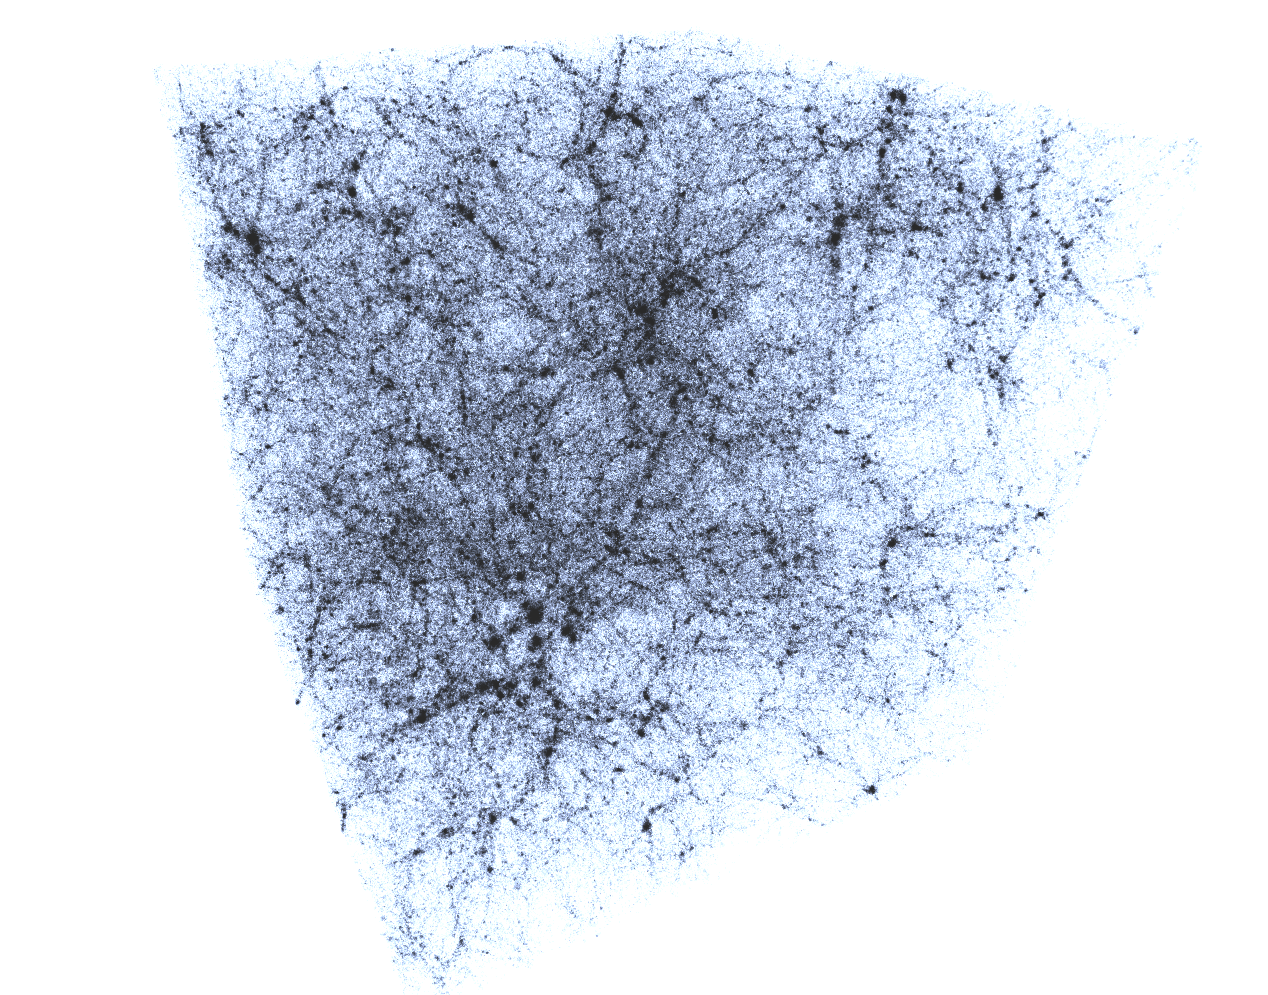
\includegraphics[width = \linewidth]{Figures/Chapter1/DMStruct.png}
    \caption{A visualization of the `cosmic web'. The shading shows the distribution of dark matter. The darkest regions are the spherical `halos' between the halos extended filaments can be seen. Regions of note are the void in the upper right and the clusters in the top middle and lower left, initially the dark matter density field would have been simmilar to the microwave background but giga-years of collapse have accentuated small features into large structure. Image Credit: C.Marsden using the galaxy and structure visualization code Astera processing the Bolshoi Planck dark matter simulation (https://astera.soton.ac.uk/).}
	\label{fig:DMStruct}
\end{figure}

%Halo Finders, Halo mass functions, Merger Trees and EPS formalism
In order to analyse complex dark matter simulations several classifications have been developed to describe the dark matter haloes. Firstly, `virialised haloes' collections of dark matter particles\footnote{Note here a dark matter particle is a simulation element, often millions of solar masses, and not the theorised fundamental particle.} that are balanced in terms of their potential and kinetic energy, mathematically, 
\begin{equation}
    \langle T \rangle = -\frac{1}{2}\sum^{N}_{k=1}\langle \mathbf{F}_k \cdot \mathbf{r}_k \rangle.
\end{equation}
Secondly, from a structural point of view haloes can be defined by their over-density. 
Specifically a halo is defined as a sphere containing a density of mass that is a set number times that of a defined average density. The average density definitions commonly used are defined by either the background\footnote{The average density of the Universe.} or critical\footnote{The density required such that the universe will not expand forever.} density.
For example $M_{200c}$ would be the mass of a halo where the halo is defined as the spherical region that is 200 times the critical density. To identify these regions a number of methods have been devloped:

\begin{itemize}
    \item Bound Density Maximum: BDM classifies halo structure by defining a spherical over density threshold, e.g. $M_{200c}$, then removes particles that exceed the escape velocity of the halo mass \citep{Klypin1997Particle-MeshSimulations}.
    \item Friends of Friends: FOF uses a dark matter particle linking threshold, particles are `linked' together if they are closer than the threshold. One particle cannot be in two FOF groups simultaneously such that particle groups are unique \citep{Davis1985THEMATTER}.
    \item ROCKSTAR (Robust Overdensity Calculation using K-Space Topologically Adaptive Refinement): ROCKSTAR is a cutting-edge development of the FOF halo finders. Using a 6-dimensional phase space and a temporal dimension the structure and evolution of haloes are extracted from dark matter simulations \citep{Behroozi2011TheCores}.
\end{itemize}

Once equipped with a halo classification and an extraction tool a language and formalism to describe how these structures relate to one another is required. Hierarchical assembly predicts halo growth via accretion followed by cannibalisation of a smaller halo, this process is not instant and during this time the smaller halo is situated within the larger and can be refereed to as a subhalo. Subhaloes then may contain further structure from smaller halos they have accreted. Thus there are different `orders' of halos: $0^{th}$ order or central halos, $1^{st}$ order or sub-halos whose parent is a $0^{th}$ order halo, $2^{nd}$ order or sub-halos whose parent is a $1^{st}$ order halo, and so on. Useful statistical descriptions of the haloes are the halo and subhalo mass functions. The halo mass function is defined as the number density of central haloes of a given mass per unit volume. The subhalo mass function has multiple definitions depending on the definition of subhalo each definition is useful to a different context. Firstly, one can define the global subhalo mass function, similarly to the halo mass function this is the number density of subhaloes at a given mass per unit volume. Secondly, one can define the subhalo mass function relative to a particular central host halo, which provides the number of subhaloes of a given mass ratio $M_{subhalo}/M_{central}$ one expects to be associated to a halo mass $M_{central}$. 


Once a subhalo has been accreted onto a central halo it begins the process of merging. As the subhalo orbits it gradually loses mass to the parent halo due to tidal disruption. This process is called `stripping', initially the outer regions of the subhalo are stripped with the denser centre remaining for longer. Once a subhalo can no longer be resolved by the simulation, and its mass indistinguishable from the parent halo's mass it is regarded as fully merged. Information on this process is learnt from using the aforementioned halo finders to track substructures between simulation snapshots. As this is a simulated result it is important to note that the simulation calibration, e.g. number of particles and force softening, can strongly affect the timescale of subhalo disruption \cite{vandenBosch2018DarkDisruption}.

As the subhaloes are an evolving population, it is necessary to state which subhalo mass definition one is using:

\begin{itemize}
    \item Unevolved Subhalo Mass Function (USHMF): This mass function is the total number of subhaloes that have accreted onto a central halo over its entire history. The subhalo mass is defined at the point of accretion and is frozen at infall and no number density is ever lost. This mass function is useful for understanding the total accretion history of a halo.
    \item Unevolved Surviving Subhalo Mass Function (USSHMF): This mass function is the total number of subhaloes that reside in a halo at a given epoch. Subhaloes once accreted are frozen in mass, however, at the time when they would have fully merged are then considered removed from the count. This mass function is useful as it retains information about the infall masses and can be further categorised to retain information about number density contribution from different infall epochs.
    \item Evolved Subhalo Mass function (ESHMF): This mass function is the total number of subhaloes that reside in a halo at a given epoch where the subhaloes have undergone mass loss/transfer to the central halo. This mass function is the `true' subhalo mass function that one would expect to see if dark matter were directly testable e.g. via galaxy lensing in groups and clusters \cite{Bartelmann2001WeakLensing}.
\end{itemize}

In Figure \ref{fig:SubHaloes_byz}, in the left-hand panel we show the halo mass function at redshift $z=0.1$. Note the characteristic schechter function shape with an inverse linear relationship between number density and halo mass in log-log space, which breaks and rapidly declines above a threshold mass, which at this redshift is roughly $M_h\sim 10^{14}$ $M_{\odot}$. In the right-hand panel we show the Global Unevolved Surviving Subhalo Mass Function at redshift $z=0.1$. In both panels the coloured shading represents contribution to the global USSHMF at different redshifts of infall, note the logarithmic scaling means the shading is not linear. Recent accretion is the dominant contributor of subhaloes at all masses. Furthermore, high mass subhaloes $M_h \geq 10^{13} M_{\odot}$ accrete only at redshifts below $z < 2$.

\begin{figure}[h]
	\centering
	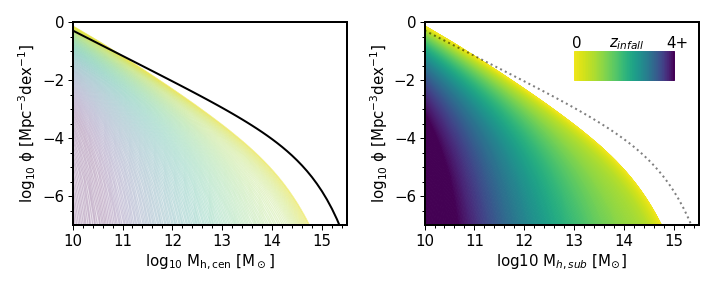
\includegraphics[width = \linewidth]{Figures/Chapter1/SubHaloes_byz.png}
    \caption{Left: Central Halo Mass function, the global number density of haloes at redshift $z=0.1$. Right: Global Unevolved Surviving Subhalo Mass Function at redshift $z=0.1$. The colour gradient shows the fraction of subhaloes at each mass coloured by redshift of infall. Note due to the logarithmic scaling the thinner yellow bar at the top of the distribution is a majority contribution of subhaloes, showing that at all masses recent accretion dominates the population.}
	\label{fig:SubHaloes_byz}
\end{figure}

In addition to the distinction between central and satellite haloes, information about the full mass assembly is also extracted from simulations. Halo assembly histories are commonly visualised as simple(\textit{ish}) tree networks, referred to as a ``merger trees''. Central haloes are identified at a low redshift and the main progenitors followed backwards in time to create the central `trunk'. At any epoch where a merger occurs, the main progenitor is assigned to be the larger of the two merging haloes\footnote{This remains true even if the main progenitor branch becomes smaller than the other branch at an earlier redshift.}. At each merger a `branch' is created following this branch which followed back in time gives the assembly history of that halo. We show an example of a simple merger tree in Figure \ref{fig:SimpleTree}.

\begin{figure}[h]
	\centering
	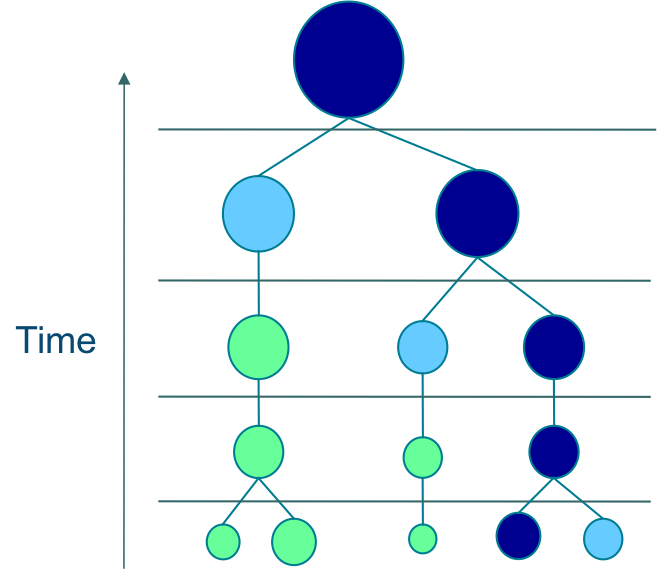
\includegraphics[width = \linewidth]{Figures/Chapter1/Merger_Tree_Simple.png}
    \caption{A cartoon of a simple merger tree. Increasing time moves up the page as indicated on the right, horizontal lines separate epochs. Dark blue circles represent the main progenitor or trunk haloes of the merger tree. Haloes that merge directly onto the trunk are coloured in light blue, the merger history or branch for each of these merging haloes is shown in green.}
	\label{fig:SimpleTree}
\end{figure}

There are increasingly more complex merger tree diagrams, it is not the case that a haloes merge simply we list some examples and show what these may look like on a stylised merger tree in Figure \ref{fig:Substructures}.

\begin{itemize}
    \item Substructure: A halo is not immediately dissolved upon accretion to the central halo, substructure is therefore maintained in central haloes between epochs. Furthermore, haloes on accretion may also carry internal substructure, which creates 2nd (and above) order substructure in the parent halo.
    \item Flyby Haloes: Some haloes may pass through another halo and may lose mass but are not captured. These haloes are known as flyby halos and must be accounted for when constructing mass functions to not inflate the number count of subhaloes.
    \item Re-Accreted Haloes: Haloes on particularly eccentric orbits or haloes with initially high velocity may enter a halo subsequently leave the halo group. These haloes whilst still bound to the group may not be associated to the group by a halo finder appearing to be flyby haloes. However, they at some later may reenter the group: Firstly, one must ensure these halos are not double counted. Secondly it caution must be taken the mass they are accreted at is fit for purpose (i.e., mass at last accretion, mass at first accretion, or peak mass).
\end{itemize}

\begin{figure}[h]
	\centering
	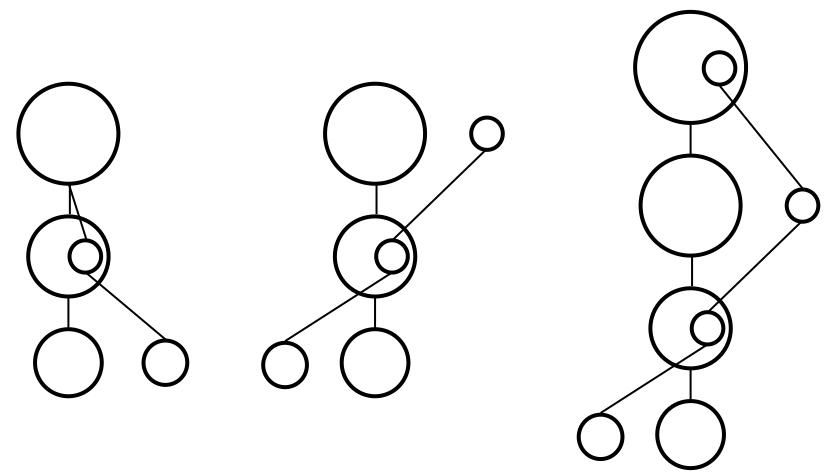
\includegraphics[width = \linewidth]{Figures/Chapter1/Substructures.png}
    \caption{From left to right: An example of: $1^{st}$ order substructure, a flyby halo and, a re-accreted halo.}
	\label{fig:Substructures}
\end{figure}

Whilst there is clearly a wealth of information available from dark matter simulations they are costly require a large amount of computational power both to run and analyse. For many models of galaxy evolution the information provided is far in excess of what is required. Press-Schechter Formalism \citep{Press1974} provides an alternative way to generate simple analytic dark matter distributions at a greatly reduced computational cost. For a simple visualisation one can consider the dark matter distribution at high redshift as a random Gaussian probability distribution. 


Peaks in this distribution represent dark matter over densities which will collapse over time where higher peaks collapse earlier due to greater gravitational influence. This can be visualised as a time evolving threshold above which the dark matter density would qualify as a collapsed halo. If the summation of two Gaussian distributions are above this threshold then they become a single over-density or halo. A simplified cartoon is shown to visualise this in Figure \ref{fig:PS_Cartoon}.

\begin{figure}[h]
	\centering
	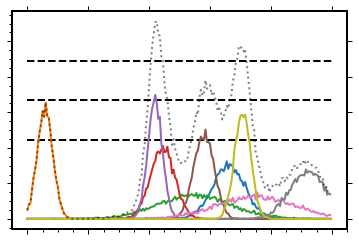
\includegraphics[width = \linewidth]{Figures/Chapter1/PS_Cartoon.png}
    \caption{A visualisation of the core theory of Press-Schechter Formalism. The solid coloured lines are random Gaussian distributions representing fluctuations in the initial mass density field, the grey dotted line is the total mass distribution. The three black dashed lines are for visualising the threshold of collapse at different epochs. The x-axis is an arbitrary spatial dimension, and the y-axis an arbitrary density unit.}
	\label{fig:PS_Cartoon}
\end{figure}

Following Figure \ref{fig:PS_Cartoon} considering the top dashed line as the earliest epoch we look for collapsed haloes by examining the dashed line; two peaks in the density field can be found above above the threshold denoting two collapsed halo structures. The area above the threshold is analogous to the mass of the halo and the spread of the peak analogous to the size. At the second threshold there is another collapsed peak mostly contributed by the brown Gaussian. Furthermore, the two peaks from the first collapse have grown in mass as can be seen by an increased area and spatial extent. Finally, looking at the last collapse threshold: On the left there is a new isolated peak; on the right the peaks created by the yellow and brown Gaussian distributions now create one continuous area above the threshold, this is an indication of two merged haloes. Within this merged halo there are two distinct peaks that can indicate the nature of the halo substructure. It evident that at later epochs the merged substructures will also include the purple peak. This picture is a oversimplification of Press-Schechter Formalism, the Gaussian field is actually significantly more interesting the density fluctuations mirror the distribution of the cosmic microwave background. Furthermore, instead of simple collapse thresholds a window function is used to smooth the density field. Finally, here the peaks are represented as static, however, their size and location will evolve with time. The shift in the peaks location can be used to build dynamic halo histories without the need for full N-Body simulations \cite{Voivodic2019ExcursionCatalogues}.

The Press-Schechter Formalism can be used to analytically create a merger tree by utilising the probability of any two over densities merging. An algorithm that starting at a given redshift with a given halo mass can then construct a theoretically valid merger history. We summarise here the \textsc{galform} \citep{Cole2000} algorithm for making merger trees from Press-Schechter Formalism\footnote{In \citet{Parkinson2008GeneratingTrees} improvements to this method are proposed to better align the generated merger trees with the millennium simulation by using a perturbing function to remove systematic differences between N-Body simulations and the algorithm.}.

\begin{itemize}
    \item Pick a starting Mass, $M_{h}$ and redshift $z$. This will be the final mass/redshift for the main progenitor halo in the tree.
    \item Step backwards in redshift in steps, $dz$, where $dz$ is chosen that the probability, $P$, of a halo having a merger in $dz$ is $P\ll1$.
    \item Generate a uniform random number, $N$, if $N<P$ the halo splits, else the mass is reduced to account for unresolved haloes or smooth accretion and the process repeats.
    \item If the halo has split a random number is generated from the probability distribution that defines the possible progenitor halo masses from  Press-Schechter Formalism this is the mass of the split halo, $M_{split}$. The central halo mass is then updated to be less the split mass and a smooth/unresolved accretion component and the process repeated.
\end{itemize}

The merger trees generated using this algorithm are simpler and less computationally expensive than those extracted from N-Body simulations, and if calibrated properly fully consistent with \LCDM cosmology. They therefore are an ideal choice for simulations that need to generate halo merger trees on demand.

%How do these predictions effect galaxy assembly
Dark matter interacts with baryonic matter via gravity. As dark matter is five times more abundant than normal matter it is the dominant gravitational force in the universe. In a \LCDM universe baryonic matter traces the dark matter distribution. Galaxies are thought to assemble at the centre of dark matter halos where gas accumulates, the larger the halo the larger quantity of gas collects in the halo and the larger the galaxy. The hierarchical assembly of dark matter halos is then translated into the galaxy population. Galaxies will follow the merger history of their host haloes, smaller galaxies will follow their host subhalo when it merges with a larger central halo. Massive galaxies, that reside in massive haloes that have many halo mergers, are expected to be surrounded by many smaller satellite galaxies. These satellite galaxies along with their host sub haloes will loose angular momentum to the central halo and eventually merge with the central galaxy.

\section{Hydrodynamic and N-Body Simulations}
\label{sec:Hydro}
%What is Hydrodynamics or N body
Hydrodynamical simulations are the most `real' galaxy simulation. Within a volume dark matter, gas, and stars are assigned to particles and/or grid cells, forces are then applies to each element with respect to each other element. The volume is then solved by repeated solving and time stepping and snapshots produced at set intervals to be used for analysis. Processes that take place below the resolution limit of the simulation, such as starformation, are simulated using a sub-grid routine based on the properties of the given volume element.

%State of the Art
\subsection{State of the art: Illustris TNG}
The Illustris TNG simulations are a suite of 18 simulations, they use three different volumes, $\sim 50, 100, 300$ ${Mpc}^{3}$, and study a range of physical complexity and resolutions. TNG at its core use the code \textsc{arepo} \citep{Springel2010EMesh} which solves coupled ideal magneto-hydrodynamics and self gravity using periodic boundary conditions. Even for TNG50 where exceptionally high resolution for a cosmological simulation is achieved much of the baryonic physics falls below the resolution limit, this physics in then included via so called `sub-grid' models. Sub-Grid models are used for star formation, super massive black holes, galaxy feedback process (starformation and AGN) and more. A specific example of one such sub-grid model is star formation, gas above a threshold density $n_H \simeq 0.1cm^{-3}$ is allowed to form stars following the results of \citet{Springel2003CosmologicalFormation}. Sub-grid models attempted to replicate results from smaller higher resolution simulations or from observations. 

%Drawbacks
\subsection{Pros and Cons}
The drawbacks of using a hydrodynamic model are foremost limitations of resources, they require vast amounts of computational resource to run and take a lot of developer time and skill to create. Furthermore, they create huge amounts of output data that can be difficult to process and interpret. The combination of these effects result in a simulations that have volume and resolution constraints. For example the TNG simulations run three box sizes such that the larger boxes can simulate rare/low abundance objects and the smaller boxes can simulate galaxies in high detail, the computational time to run a simulation that produces both would make the computational cost impractical and the data products unmanageable. 

The advantages of explicit modelling through hydrodynamics is that one can study the dynamics and interactions of the particles that make up galaxy directly. Furthermore, by carefully choosing the size and resolution of the simulation it is possible to understand there details over many orders of magnitude. For example, in TNG one explores how the cosmological environment effects galaxy formation, the study of gas flow along dark matter filaments and understand the statistics of galaxy mergers. Alternately in FIRE one high resolution `zoom in' region is simulated with high fidelity, the resolution is such that feedback from starformation winds, AGN, and even individual supernovae are resolved. Whilst hydrodynamics represent the stare of the art in our ability to simulate a universe or a individual galaxy in a holistic manner the time and difficulty mean they are not the ideal tool for testing they cannot be easily re-run and are therefore not ideal as laboratories to test ideas. 

Progress has been made in each aspect that limits hydrodynamics, firstly, the speed, memory and architecture of compute resources continues to improve with recent advances in GPU technology contributing to the overall power available to simulators. In addition to this novel techniques such as genetic modification whereby the initial conditions of a simulation are subtly altered to test how perturbations and modelling assumptions effect self simmilar galaxies \citep{Pontzen2017HowGalaxy}. Building on these advances in speed and flexibility it may well become possible to use hydrodynamic simulations as comprehensive tools, but as it stands we are still reliant on complimentary tools such as semi-analytic and semi-empirical modelling.

\section{Semi-Analytic Modeling}
\label{sec:SAM}
%What is a SAM
\subsection{History of Semi-Analytic Models}
Building off the hierarchical collapse models from \LCDM cosmology and the power of generating merger trees from EPS routines \citep{Press1974} a new form of galaxy model was conceived. The dark-universe was conceived of from the rotation curves of galaxies it followed that galaxies follow the structure formation of the dark matter haloes predicted in \LCDM cosmology. The earliest models successfully recreated the galaxy luminosity function by assigning baryonic matter to EPS haloes and solving analytic gas collapse equations \citep{White1978CoreClustering}.

%Brief aside on the simple analytics here?

Semi-analytic models were then developed and extended to include more advanced galaxy physics, such as the formation of galaxy disks \citep{Mo1998TheDiscs}. Increasing in complexity by both folding in more advanced physics such as AGN feedback and using merger trees form N-body dark matter simulations the models were able to increase the scope of predictions by tuning parameters over several simulation runs to best fit the observations \citep{Bower2006BreakingFormation}. Continuing improvements in cosmological (dark matter) simulations have allowed for semi-analytic models to improve both in resolution and size. In addition, as computing power has become cheaper and better monti-carlo methods have been developed, this has allowed for the popularisation of the multi-parameter semi-analytic models tuned over hundreds or thousands of runs \citep{Guo2011FromCosmology,DeLucia2011TimesCosmology,Fontanot2011TheUniverse,Menci2014TriggeringInteractions,Somerville2015StarGas}.
In this section we will discuss the state of the art in semi-analytic modelling by summarizing a review by \citet{Somerville2015StarGas} followed by deconstructing a subset of the latest models and finally present a consideration the drawbacks of semi-analytic models compared to other galaxy modelling techniques.

\subsubsection{Somerville (2015) Review \citep{Somerville2015StarGas}}
\textit{The semi-analytic models used here have been described in detail in Somerville \& Primack (1999), Somerville et al. (2001) and most recently in Somerville et al. (2008a, hereafter S08) and Somerville et al. (2012, S12). The Santa Cruz modelling framework has also recently been described in Porter et al. (2014). We refer the reader to those papers for details.}

This review explores 3 models published in \citet{Somerville2008ANuclei} (hereafter S08), \citet{Somerville2012GalaxyObservations} (hereafter S12), \citet{Porter2014ModellingSpace} (hereafter Santa Cruz). Each of these models is run using EPS merger trees as a backbone. Using analytic merger trees allows for high resolution reducing the minimum halo size capturing small galaxies that pose semi-analytic models difficulty at redshifts $z = 0.5 - 2$. Galaxies grow via the cooling of gas from re-ionization, before this point haloes are seeded with gas at the cosmic baryon fraction. After this gas cools as given in \cite{White1991GalaxyClustering} this gas condenses and forms stars at the center of dark matter haloes. 

The prescriptions made to handle the hierarchical assembly predicted by \LCDM cosmology concern firstly the halo structures. At the point of halo merger the larger halo and associated galaxy are assigned as the central, the smaller halo(es) and associated galaxies become sub-haloes and satellite galaxies creating the substructure seen around galaxies. Satellite galaxies then merge with the central galaxies on timescales given by the Chandrasekhar formula \citep{Chandrasekhar1943DYNAMICALFRICTION} as given in \citet{Boylan-Kolchin2008}. The mergers of satellites with the central galaxies gradually transform the morphologies of the central galaxies by reducing the central galaxies angular momentum eventually creating a spheroid \cite{Hopkins2009HOWMERGERS}. 

In addition to changing the morphologies of central galaxies mergers are also thought to drive one of the two pathways of star formation. During a merger as the gas of the two merging galaxies is disrupted the galaxies can undergo a starburst, a short period where star formation is enhanced by an order of magnitude \citep{Hopkins2009HOWMERGERS}. The second mode of star formation is referred to as 'disk mode' and is investigated using three models: The Kennicutt Schmitt \citep{KennicuttJr.1998TheGalaxies} assumes the surface density of starformation, $\Sigma_{SFR}$, is related to the surface density of cold neutral gas, $\Sigma_{gas}$,

\begin{equation}
    \Sigma_{SFR} = A_{SF}\Sigma_{gas}^{N_{SF}}.
\end{equation}

It is here and in the following star formation rate recipes that the first tuning parameters $A_{SF}$ and $N_{SF}$ are found; they control respectively the normalisation and slope of the star formation rate. In addition to these there are two critical gas densities $\Sigma_{crit}$ and $\Sigma_{H2,crit}$, that below which neutral gas or molecular gas will not form stars. Similar to the Kennicutt Schmitt recipe molecular gas star formation follows empirical results that link the molecular gas surface density to the star formation rate simply from \citet{Bigiel2008TheResolution},

\begin{equation}
    \Sigma_{\mathrm{SFR}}=\left(\frac{A_{\mathrm{SF}}}{10 M_{\odot \mathrm{PC}^{-2}}}\right) \Sigma_{\mathrm{H}_{2}} N_{\mathrm{SF}}.
\end{equation}

Its observed that above a critical H2 density the SFR steepens \citep{Narayanan2012ALaw} the SFR is also modeled using a two part scaling law,

\begin{equation}
    \Sigma_{\mathrm{SFR}}=A_{\mathrm{SF}}\left(\frac{\Sigma_{\mathrm{H}_{2}}}{10 M_{\odot \mathrm{pc}^{-2}}}\right)\left(1+\frac{\Sigma_{H_{2}}}{\Sigma_{\mathrm{H}_{2}, \mathrm{crit}}}\right)^{N_{\mathrm{SP}}}
\end{equation}

Semi-analytic models rely on several feedback prescriptions to regulate their starformation. The energy released during supernovae created as a result of starformation is deposited in the ISM this energy drives outflows of cold gas,

\begin{equation}
    \dot{m}_{\mathrm{out}}=\epsilon_{\mathrm{SN}}\left(\frac{V_{0}}{V_{c}}\right)^{\alpha_{\mathrm{rh}}} \dot{m}_{*}.
\end{equation}

In addition to supernova feedback, AGN feedback caused by the growth of the super-massive black hole at the center of the galaxy. AGN feedback is in two modes: The first is initiated after a galaxy merger, as the black hole grows energy is released to the ISM until the accretion is balanced by outflows from the black hole. In this mode the gradual heating of the ISM reduces the SFR by heating the cold gas reservoir. The second black hole growth mode, ``radio mode'' from cold core gas from the galactic nucleus cause an accretion disk following the \citet{Bondi1952OnAccretion} model. This launches a jet that couples with the halo gas preventing the gas from cooling and falling onto the central galaxy where it could form stars.

A further consideration taken in semi-analytic modelling, is the state of the gas. The state can be calculated in several different ways, an empirical pressure based relationship is given by \citet{Blitz2006TheRelation}, the pressure in the disk is related to the ratio of molecular and atomic hydrogen. 

\begin{equation}
    R_{\mathrm{H}_{2}}=\left(\frac{\Sigma_{\mathrm{H}_{2}}}{\Sigma_{\mathrm{HI}}}\right)=\left(\frac{P_{m}}{P_{0}}\right)^{\alpha}
\end{equation}

The $H_1$ \& $H_2$ surface densities are given by $\Sigma_{\mathrm{HI}}$ \& $\Sigma_{\mathrm{H}_{2}}$, $P_m$ is the mid disk pressure, and $P_0$ \& $\alpha$ are additional free parameters. The gas partitioning can be calculated though an analytic model based on the connection between the interstellar radiation filed and the molecular self shielding \citep{Krumholz2008TheClouds,Krumholz2009THEDENSITIES,Krumholz2009THEGAS},

\begin{equation}
    f_{H_{2}}=1-\left[1+\left(\frac{3}{4} \frac{s}{1+\delta}\right)^{-5}\right]^{-1 / 5}
\end{equation}.

This is by no means a complete record of the various analytic recipes used in semi-analytic modelling. However here we have shown a subset of the multitude of free parameters that enable tuning of such models to achieve results consistent with observations.

\begin{equation}
s=\ln (1+0.6 \chi) /\left(0.04 \Sigma_{\operatorname{comp}, 0} Z^{\prime}\right),
\end{equation}
\begin{equation}
\delta=0.0712\left(0.1 s^{-1}+0.675\right)^{-2.8},
\end{equation}
\begin{equation}
\chi=0.77\left(1+3.1 Z^{\prime0.365}\right),
\end{equation}
where $\Sigma_{\operatorname{comp}}$ is the surface density for a given 100pc atomic-molecular cloud.

The final mechanism we discuss here is the enrichment of the galaxy and halo gas with metals. During the process of star formation and stellar mass recycling metals are created. This is modelled as a batch process where $\mathrm{d} M_{Z}=y \mathrm{d} m_{*}$ where a mass $\mathrm{d} M_{Z}$ of metals is produced in each batch of star formation $\mathrm{d} m_{*}$, $y$ is a free parameter. The metal enriched gas formed in this process is ejected by supernovae and assume instantaneously mixed with the cold disk gas. As supernovae are though to be one of the main drivers of galactic wind the metals are thought to be preferentially ejected with the wind $\zeta$ paramatises the ejected metal fraction, and the equation for the metal mass in the galaxy is updated as such,

\begin{equation}
\zeta=\zeta_{\mathrm{lo}} \exp \left(-M_{h} / M_{\mathrm{ret}}\right),
\end{equation}

\begin{equation}
\dot{M}_{Z}=y(1-R)(1-\zeta) \dot{m}_{*}+Z_{\text {hot }} \dot{m}_{\text {inf }}-Z_{\text {cold }} \dot{m}_{\text {out }},
\end{equation}

$\zeta_{10}$ and $M_{\mathrm{ret}}$ are free parameters, R is the recycled fraction and $Z_{\text {cold }}$ is the metallicity of the cold gas.


%State of the art SAM
\subsection{State of the art}
Modern semi-analytic models are arguably reaching a plateau in usefulness, many were conceived in the mid two-thousands and have been iterated on for over a decade. During this time the amount, quality and availability of comparison data has increased several orders of magnitude. The maturing models have been refit with many physical prescriptions to model a wide variety of observations but many still struggle to reproduce the basics of galaxy evolution such as the evolution of the stellar mass function \cite{Asquith2018CosmicModels}. Here we briefly discuss two state of the art models that represent the cutting edge of semi-analytic galaxy modelling.

\subsubsection{GAEA}
%Hirschmann2016GalaxyModel
The GAEA model is a good example of a mature semi-analytic model originally described in \citet{DeLucia2007TheGalaxies} to model the assembly time of BCGs. It has subsequently been updated many times in 2008 (De Lucia \& Helmi) 2010 (Li et al.) 2014 (De Lucia et al.) and \citet{Hirschmann2016GalaxyModel} (see references within).
%Zoldan2019TheEvolution
One of the latest renditions of this model based on that of \citep{Xie2017H2-basedFormation} and updated in \citep{Zoldan2019TheEvolution}. This latest version of the model adds a description of quasar driven winds in an effort to model the size mass relation for both early and late type galaxies.

\subsubsection{SHARK}
%lagos 2018 Li et al.
%lagos 2019
The SHARK semi-analytic model represents a push to keep the field of semi-analytic models in line with current software engineering best practice. The release paper \citep{Lagos2018Shark:Formation} carefully details the physical prescriptions and modularity that defines the code. SHARK is designed to be flexible and modular and takes pride in being the most accessible open source code available. In \citet{Lagos2018Shark:Formation} the authors show the baseline performance of SHARK to be as good as or exceeding other semi-analytic models in the mass-size, gas-stellar mass and stellar mass-metallicity relations. The flexibility of SHARK is then demonstrated in \citet{Lagos2019FromModel} where  shark is modified to use different dust mass models to match spectral energy distribution observations of galaxy emission from the far-UV to the far-IR.

%Drawbacks of SAM
\subsection{Drawbacks of Semi-Analytic Modeling}
A major component of a Semi-Analytic model is the number of parameters that can be tuned to reproduce observations, for example the default SHARK configuration has over 50 parameters defined. Whilst the breadth of these parameters allows for semi-analytic models to produce fits to a wide range of observational properties where multiple parameters can both affect the same observable degeneracies that obscure the actual physics arise during the tuning process \citep{Lapi2011DarkModels,Gonzalez2011Evolution4}.


\section{Semi-Empirical Modelling}
\label{sec:SEM}
%What is a SEM
Semi-empirical models similarly to semi-analytic models are built on prepossessed dark matter accretion. A semi-empirical model additionally uses observations as an input. By comparing the relative abundance of dark matter haloes and observed galaxies a correlation between halo mass and stellar mass is determined \citep{Kravtsov2004TheDistribution,Shankar2006NewFormation}. This process is called abundance matching and is explained in greater depth in Section \ref{C2:SubSec:AbnMtch}. When used correctly abundance matching ensures that semi empirical models recreate the observed distributions of galaxies over many redshift epochs. Constraining galaxy masses and other properties via observations significantly reduces the parameter search space compared to hydro-dynamical or semi-analytic models. In doing so semi-empirical models are able to probe areas of physics that may not yet have clear constraint or physical mechanism.

Since there inception semi-empirical models have grown in complexity and with this increased their parametrization, even approaching the levels of semi-analytic models. However semi-empirical models retain more flexibility and transparency. Where the complexity of the models is controlled by observational priors and the model is internally consistent it is possible to accurately probe very specific aspects of galaxy formation whereas in models that require tuning to fit observations subtle effects can be missed in degeneracies. It is even possible to make models where the observational priors, and by extension the model, are not consistent. For example the observed stellar mass function for a long time has been inconsistent with the observed star formation rate \citep{Leja2015ReconcilingFunction,Lapi2017StellarEquation}, in this regard the semi-empirical model could use an empirical relation to show what the observed starformation rate would be without needing the conflicting measurement to form a physical part of the model. Similar yet unappreciated effects involving systematics in galaxy assembly make up a significant parts of Chapters \ref{Chapter:GalGrowth} \& \ref{Chapter:GalPairs}.

\subsection{State of the art}
Here we describe three state of the art semi-empirical models. Each of the models described here has a radically different approach to semi-empirical modelling. They are each constrained by observational priors and make predictions about the buildup of mass in galaxies though mergers and star formation rate. The range of approaches show the flexibility and the agreement between models shows the power of the empirical approach. 


\subsubsection{\citet{Rodriguez-Puebla2017ConstrainingProperties}}
%Aldo
In the model presented in \citet{Rodriguez-Puebla2017ConstrainingProperties} the SMHM is constrained using the 2 point correlation function and the evolution of the SMF. Using this constraint the inconsistent between observed SFR and SMF evolution are avoided. The results of this paper are exceptional constraints on the SFR and quenched fraction of galaxies in multi-parameter space, in both halo mass - redshift space and stellar mass - redshift space as shown in Figure \ref{fig:RP_fig}.

%Figure
\begin{figure}[h]
    \centering
    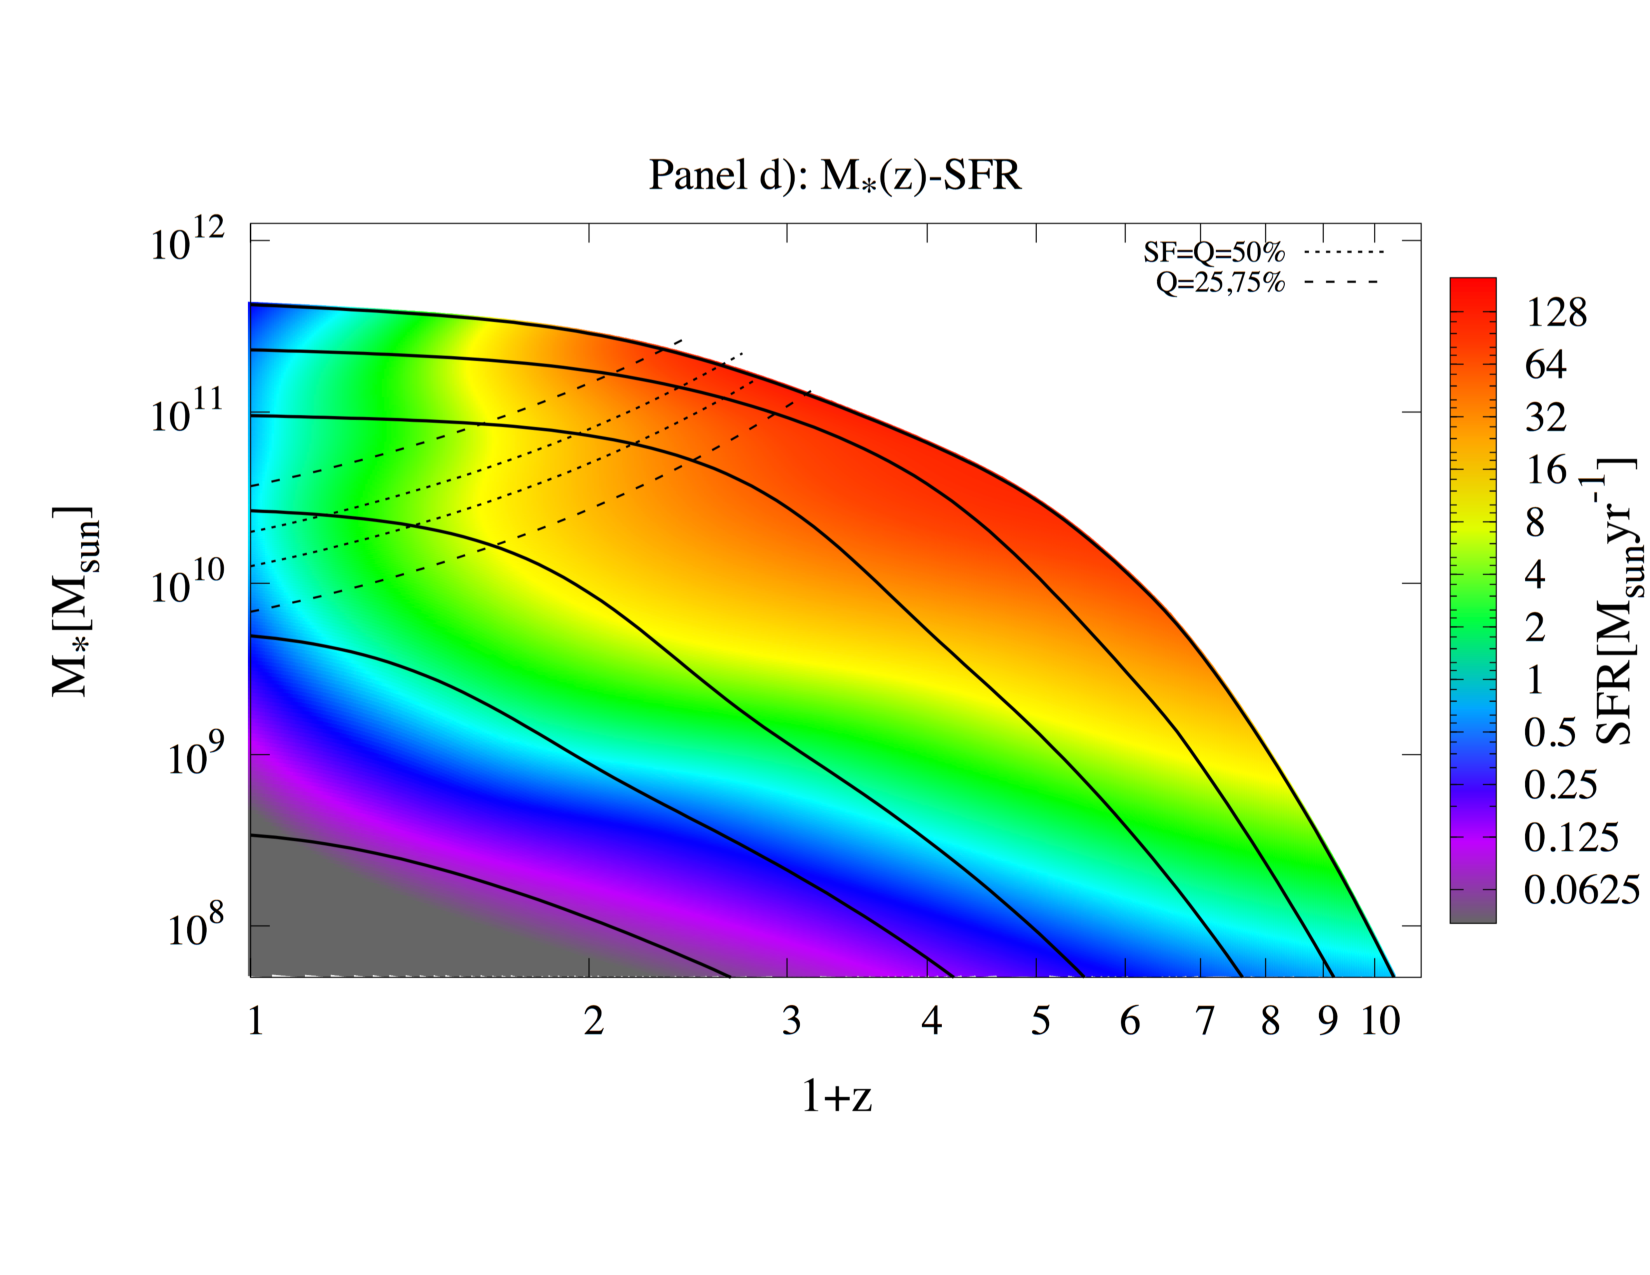
\includegraphics[width = \linewidth]{Figures/Chapter1/RP17_fig9.pdf}
    \caption{Image used with permission from: Aldo Rodriguez Puebla \cite{Rodriguez-Puebla2017ConstrainingProperties}}
    \label{fig:RP_fig}
\end{figure}


The key findings are that most stellar mass is built up in-situ at high redshift. Massive galaxies then quench at the point where the sSFR is equal to the specific halo mass accretion rate which happens at $M_{vir} \sim 2 x 10^{11} M_{\odot}$.


\subsubsection{E\textsc{merge}}
%Moster Emerge
E\textsc{merge} is presented in \citet{Moster2018Emerge10} built upon N-body dark matter simulations. From the dark matter simulation each halo is tracked with its growth history and relation to other haloes recorded. E\textsc{merge} works under the core assumption that galaxies grow in conjunction with the dark matter haloes they reside in. This is achieved through coupling the star formation rate of each galaxy to the accretion rate of the host dark matter halo parameterised in the following way,

\begin{equation}
\begin{aligned} \log _{10} M_{1}(z) &=M_{0}+M_{z}(1-a)=M_{0}+M_{z} \frac{z}{z+1}, \\ \epsilon_{\mathrm{N}}(z) &=\epsilon_{0}+\epsilon_{z}(1-a)=\epsilon_{0}+\epsilon_{z} \frac{z}{z+1}, \\ \beta(z) &=\beta_{0}+\beta_{z}(1-a)=\beta_{0}+\beta_{z} \frac{z}{z+1}, \\ \gamma(z) &=\gamma_{0}, \end{aligned}
\end{equation}

where $M$, $\epsilon_{\mathrm{N}}$, $\beta$ and $\gamma$ are the characteristic mass, efficiency normalisation, low mass slope and high mass slope respectively each has a redshift evolution parameter with the exception of $\gamma$. In addition to this additional parameters are included determining; the point at which satellite galaxies are disrupted returning all mass to the ICM, the fraction of mass ejected to the ICM during a merger, and quenching parameters from \citet{Wetzel2013GalaxyUniverse}. The fractions of in-situ vs ex-situ mass build up are computed and fit by,

\begin{equation}
f_{\mathrm{acc}}(z) =f_{2} \exp \left[-f_{1}(z+1)\right] 
\end{equation}

as well as the star formation histories fit by,

\begin{equation}
\log \Psi(z) =-\log \left[\Psi_{1}(z+1)^{-\Psi_{2}}+\mathrm{e}^{\Psi_{3}(z+1)-\Psi_{4}}\right] 
\end{equation}.

Similarly to \citet{Rodriguez-Puebla2017ConstrainingProperties} it is found that stellar mass is built up in-situ until a break point at $1.1 x 10^{12} M_{\odot}$. Above this mass larger galaxies may accrete a significant proportion of their mass.

\subsubsection{U\textsc{niverse}M\textsc{achine}}
%Behroozi UnivM
U\textsc{niverse}M\textsc{achine} \cite{Behroozi2019UniverseMachine:010} is built on a background of halo merger trees extracted from the Bolshoi simulation \citep{Klypin2016,Rodriguez-Puebla2016HaloSimulations}, using the \textsc{rockstar} halo finder and the C\textsc{onsistent} T\textsc{rees} codes \cite{Behroozi2011TheCores, Behroozi2013GRAVITATIONALLYCOSMOLOGY}. There are 21 tuning aspects with 44 parameters and 6 priors using a Markov Chain Monte Carlo the parameters are fit to a large set of observations though the algorithm depicted in Figure \ref{fig:BehMeth}.

%go to here for the source https://arxiv.org/format/1806.07893
\begin{figure}[h]
    \centering
    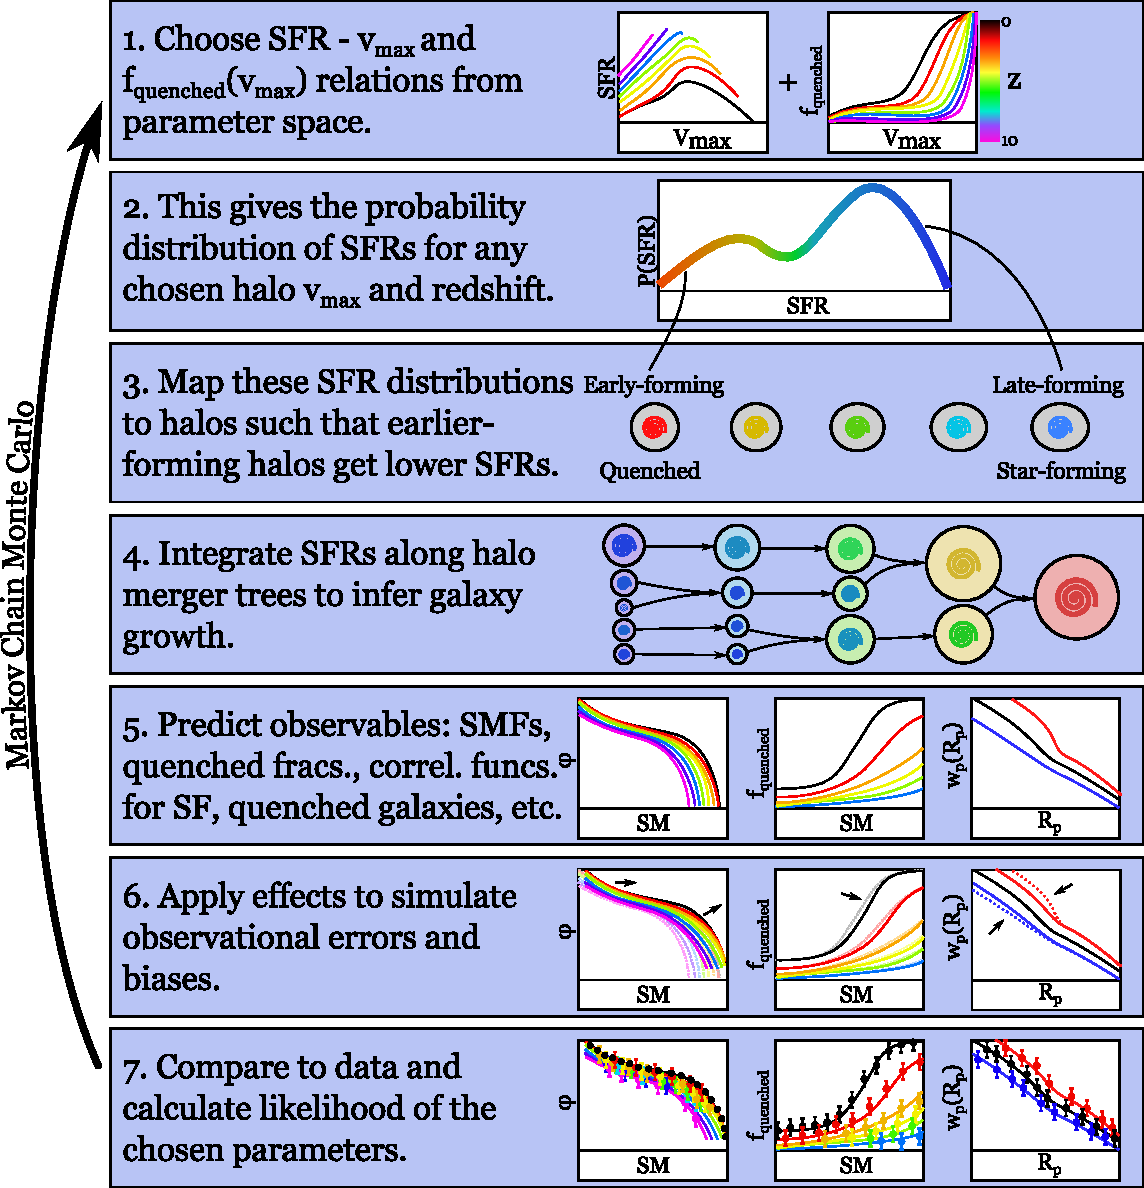
\includegraphics[width = \linewidth]{Figures/Chapter1/sfr_method.pdf}
    \caption{Image used with permission from: Peter Behroozi \cite{Behroozi2019UniverseMachine:010}}
    \label{fig:BehMeth}
\end{figure}


Using the iterative approach of parameter selection, mapping into halo structures, observable creation, through comparison to the observations the parameters are updated based on their likelihood and the process is iterated. This model is massively parallel allowing for over $10^{5}$ cores involved in any given parameter estimation. The model predictions are numerous included in which are in-situ vs ex-situ growth ratios in broad agreement with the other models.

\subsection{Limitations of the empirical technique}
%Drawbacks of SEM
Semi-empirical models as demonstrated above come in many different flavours. Each are able to draw conclusions about the connections that must exist between observational steps under given physical models. Whilst data is what empowers semi-empirical models it also presents one of semi-empirical models major limitations. Having wide and deep data sets which give statistically representative samples via large volumes to high redshift is difficult and costly. Most techniques involve correcting data sets and surveys to be consistent with one another creating a patchwork connecting the local and distant Universe. Semi-empirical models will continue to improve along with the available data although when built upon traditional dark matter simulations they share the volume constrains found in semi-analytic and hydro-dynamical models, however, this will also continue to improve with increasing computational power.


\section{Galaxy Surveys Present and Future}
\label{sec:Surveys}
Galaxy surveys are the cornerstone of semi-empirical galaxy modelling, combined with dark matter simulations they form the basis of abundance matching. Other properties such as star formation, colour, shape, size, position, e.t.c. can all form either inputs to, or constraints for the output, of semi-empirical models. It therefore stands that improving the quality of models is predicated on improving the quality of the data.

\subsection{Past and Ongoing Surveys}
Present surveys as important to semi empirical models come in two forms 'wide' and 'deep'. Wide surveys look to cover a large area of the sky to get a statistically significant look at the galaxy population. Deep surveys cover a much smaller area but using longer exposure can observe much fainter objects. The trade-off between width and depth is visualised in by a simple example in Figure \ref{fig:WvD}. Tight surveys collect more photons per unit area and can therefore see to greater depth.

\begin{figure}[h]
    \centering
    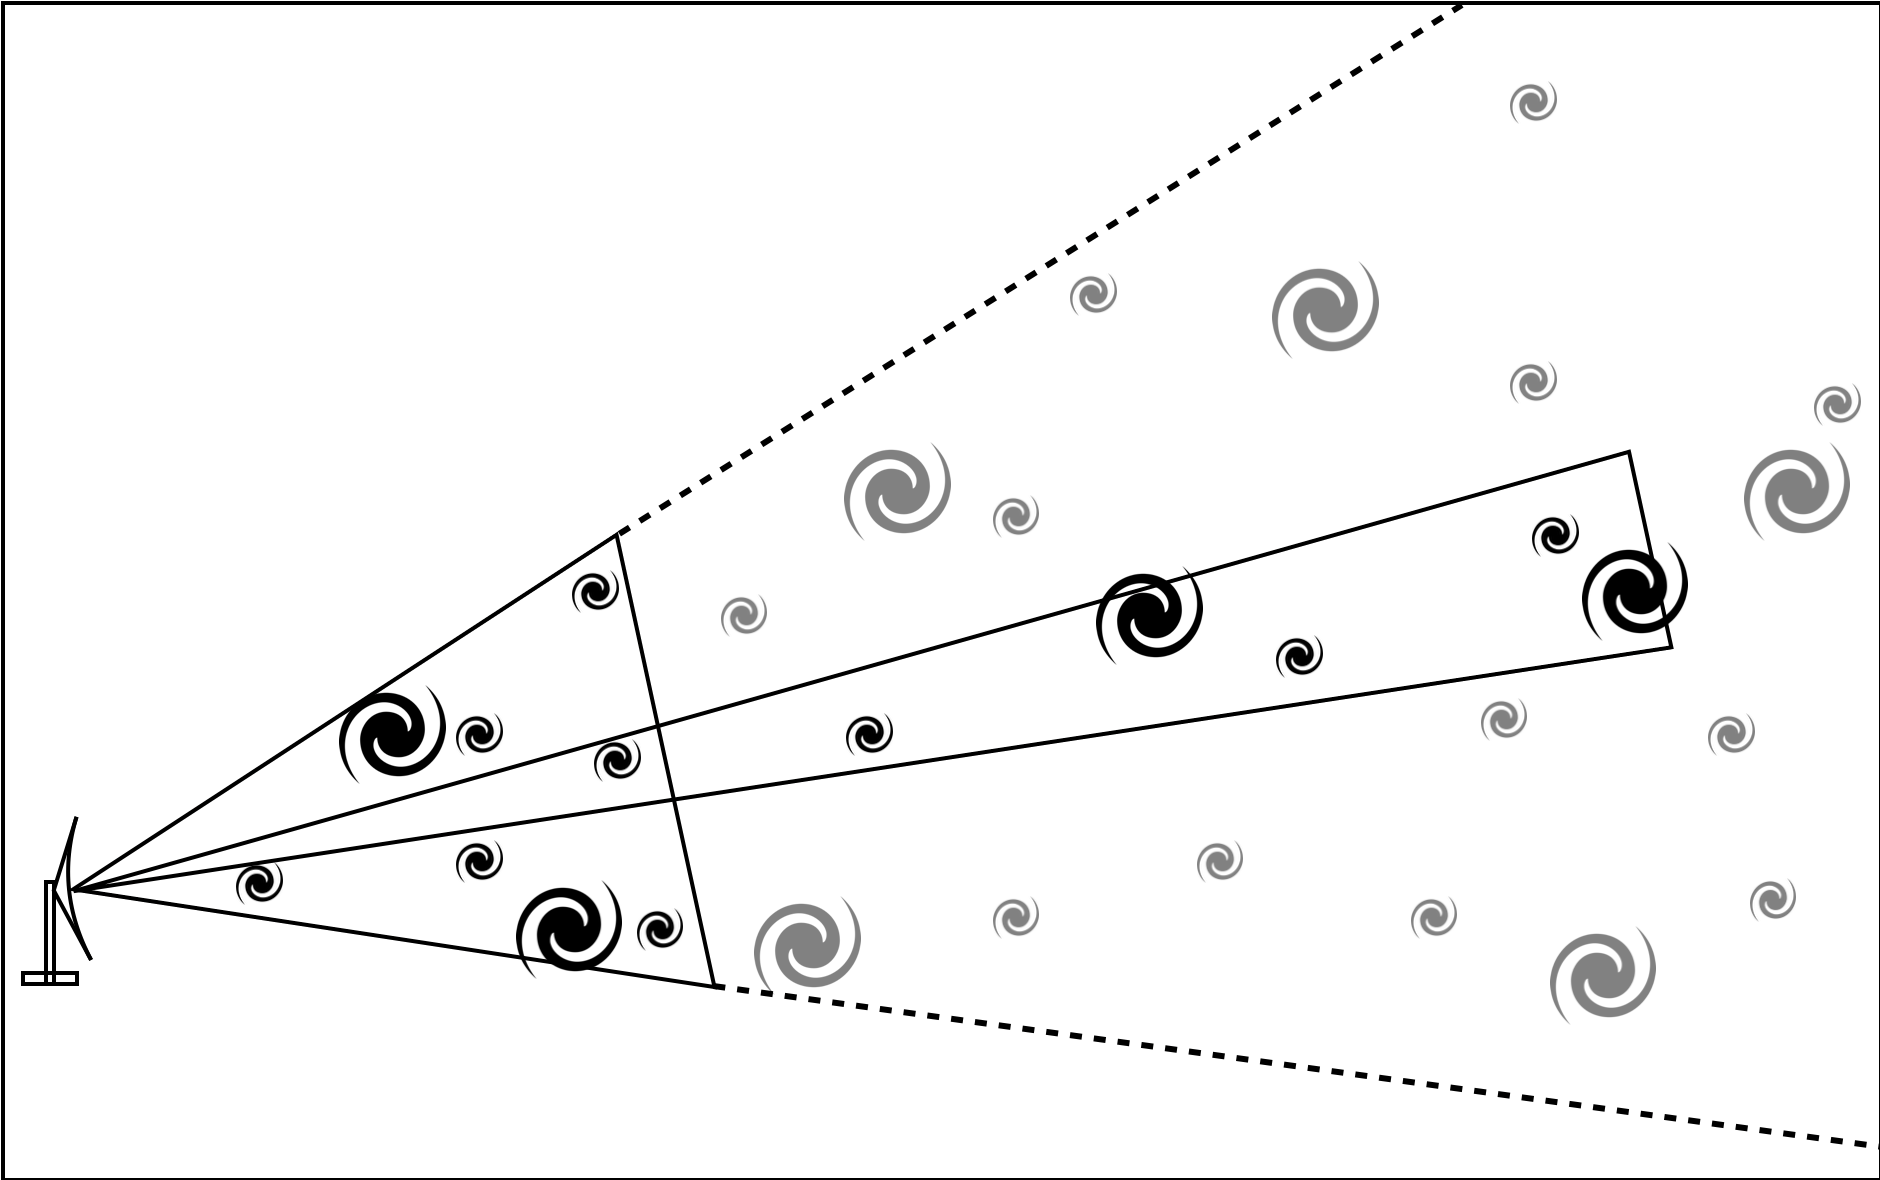
\includegraphics[width = \linewidth]{Figures/Chapter1/W_v_D_Toon.png}
    \caption{A simplified visualisation of how a trade off is made between width and depth in surveys. Given two observation areas the telescope is able to pick up galaxies to a much greater depth in narrow observation. By spending more time on one area of the sky the telescope can pick up more photons and therefore observe to a greater depth.}
    \label{fig:WvD}
\end{figure}

In addition larger galaxies are significantly brighter, the example in Figure \ref{fig:Vmax} uses two galaxy size examples. The smaller galaxies can be observed to the solid line and the larger galaxies to the dashed line. The telescope observes 6 small galaxies and 5 large galaxies, however as the larger galaxies are brighter and can be seen to greater depth. Corrections are therefore made to the number density of galaxies based on the depth that the galaxy can be observed to. In the 2D example from Figure \ref{fig:Vmax} the small galaxies can be seen in an area given by the solid area which we can call 1 unit$^2$ the larger galaxies can be seen in an area given by the dashed area that is 4 unit$^2$. In this example the smaller galaxies have a number density 6 galaxies p.u. area, the larger galaxies 1.25 galaxies p.u. area.

\begin{figure}[h]
    \centering
    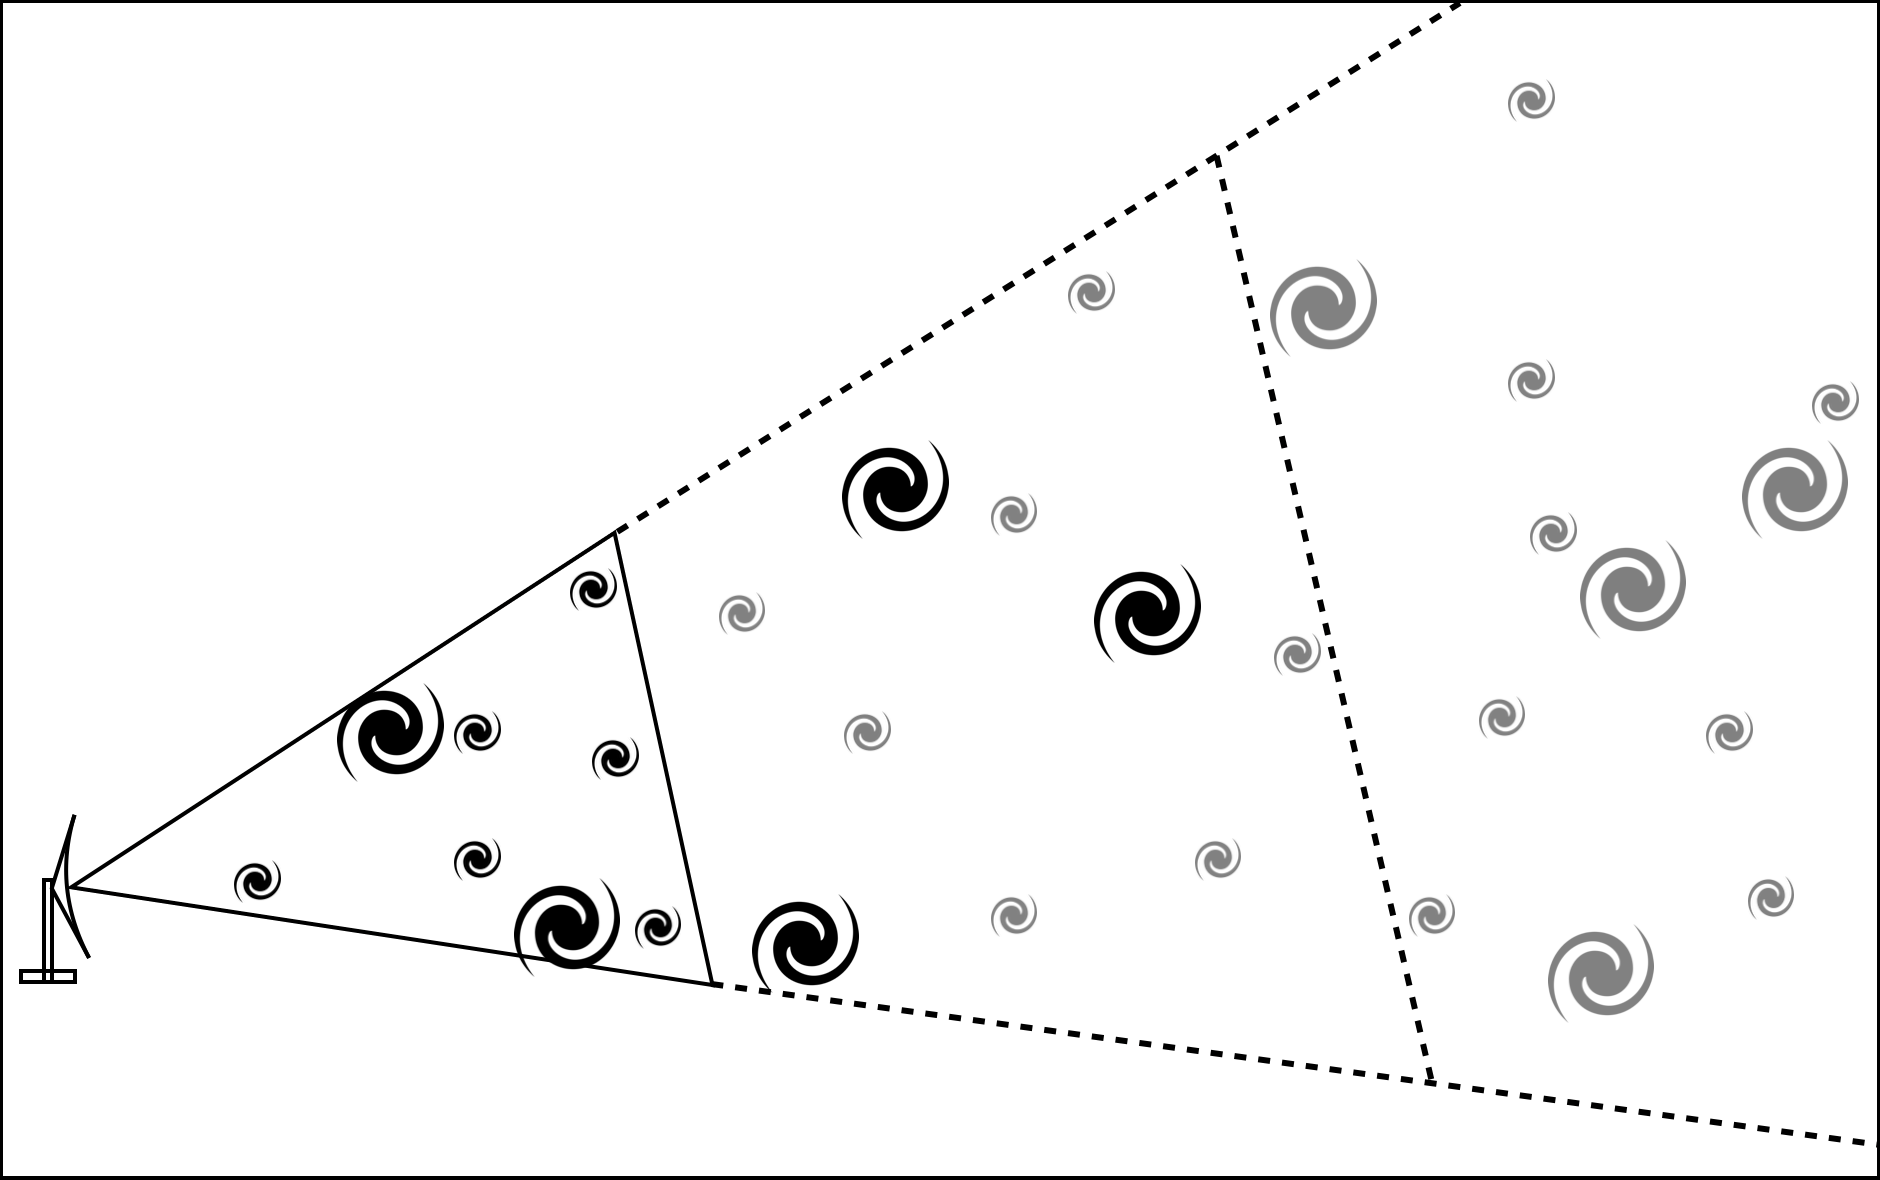
\includegraphics[width = \linewidth]{Figures/Chapter1/Vmax_Toon.png}
    \caption{A simplified visualisation of how the brightness of galaxies effects the observation depth. The smaller dimmer galaxies can be seen in the solid cone, larger and brighter galaxies can be seen up to the limits of the dashed cone.}
    \label{fig:Vmax}
\end{figure}

For each galaxy luminosity observed in a survey a correction must be made by the total depth it could have been observed to and the associated volume. In this way the volumetric density correction can be calculated for each galaxy in a given survey.

\subsubsection{Sloan Digital Sky Survey (SDSS)}

The Sloan Digital Sky Survey (SDSS) is arguably the premier wide survey for galaxies. SDSS started in 1998 with the mission to catalogue and map as much of the universe as possible. The latest release of the fourth phase is SDSS-DR19 \citep{Ahumada2019TheSpectra} now includes one-third of the night sky, it covers (u,g,r,i,z) wavelengths, has over 1.2 billion objects including over 200 million galaxies.

\subsubsection{CANDLES}
CANDLES (The Cosmic Assembly Near-infrared Deep Extragalactic Leagacy Survey) observed galaxies in the redshift range z = 8 to 1.5. CANDLES uses three Hubble Space Telescope (HST) cameras to capture emission from mid-UV to near-IR for 250,000 galaxies. The primary goals of this survey of interest to this thesis is the observation of the peak of starformation and AGN activity at $z \simeq 2$ \cite{Grogin2011Candels:Survey}.

\subsubsection{COSMOS}

COSMOS: The Cosmic Evolution Survey is a 2 square degree survey covering many wavelengths using a combination of observation from many space based and ground based telescopes (Space: Hubble, Spitzer, GALEX, XMM, Chandra, Herschel, NuStar) (Ground: Keck, Subaru, VLA, ESO-VLT, UKIRT, NOAO, Badde and Blanco, CFHT). Combining the data allows cosmos to create a rich view of the observed objects across a huge range of wavelengths. COSMOS was designed to observe galaxy evolution across cosmic time and understand the environmental effects of galaxies growing in groups and clusters \citep{HomeCOSMOS}.

\subsubsection{3D-HST}

Using 248 orbits and 124 pointings the 3D-HST is a highly complementary survey observing 625 arcminuites of previously observed extra-galactic fields \citep{Brammer20123D-HST:Telescope}. 3D-HST provides spectroscopic redshifts for over 10,000 galaxies in the range $1 < z < 3.5$. The survey provides 22 bands of rest frame colours used for the redshift catalogues, the UV-IR star formation rates and, stellar masses. The primary science goal is to investigate the evolution of galaxies at high redshifts and in combination with CANDLES be the primary spectroscopic data set until the launch of JWST.

\subsection{Future Surveys}

Due to the pace of technological advancement and the difficult and expensive nature of building (and launching in the case of space based missions) telescopes our current survey telescopes are far behind what is theoretically possible. In this subsection to of the next generation survey telescopes are described, both are space based missions being launched into orbit at the second Lagrange\footnote{The Lagrange points are 5 distinct points in a gravitational two body system at which an object can remain at rest relative to the two major bodies. In these points the forces of gravitational acceleration, centripetal acceleration and for some points the Coriolis effect are all in balance.} point 4 times the distance of the moon away from earth. The second Lagrange point is unique in its position as it sits behind the earth and is therefore permanently in the earths shadow. This positioning is ideal for satellites as it is also within the earths magneto tail and therefore experiences lower solar wind irradiation. The drawback of this point is that from here any faults that are present at launch or develop during the operation of the missions will be permanent as it is not possible to retrieve and/or fix objects sent to these points.

\subsubsection{JWST \cite{JamesNASA}}

The James Webb Space Telescope is a cold infrared telescope with a planned launch in 2021\footnote{Correct at time of writing, JWST has some notoriety for pushing this date back}. Using multi-object near-infrared spectroscopy JWST will be able to take spectra for ~100 galaxies simultaneously. Galaxies will be observed in the redshift range $1 < z < 7$ covering the peak or cosmic starformation and much of their early formation. JWST as an infrared survey is suited to looking at the starformation of galaxies, buildup of the Hubble sequence, formation of metals, effects of starbursts are all among the observational capabilities of the telescope \cite{Windhorst2009JWST2009}.  


\subsubsection{EUCLID}

The EUCLID satellite will carry two instruments VIS \& NISP between them they will cover from 500nm to 2000nm wavelengths down to the 24th magnitude, providing images of galaxies up to redshift 2. Euclid will survey 15,000 deg$^2$ of the sky and then perform a deep survey covering 40 deg$^2$ to 2 magnitudes deeper. The primary mission goals of Euclid are to address open questions on dark matter, dark energy, cosmic expansion and the formation of large scale structures \cite{Amendola2018CosmologySatellite}. To address these questions galaxies will be used as tracers of dark matter that can provide tests of cosmological models, to do this the EUCLID pipeline will contain advance galaxy cluster detection algorithms \cite{Adam2019EuclidSelection}.


\section{Original Sources}

A large fraction of this thesis is a restructuring of three papers published during PhD studies by PJG. The papers are:
\begin{itemize}
    \item \textit{`A Statistical Semi-Empirical Model: Satellite galaxies in Groups and Clusters'}  \citet{Grylls2019AClusters}, hereafter \Paper{1}
    \item \textit{`Predicting fully self-consistent satellite richness, galaxy growth and starformation rates from the STastical sEmi-Empirical modeL \textsc{steel}.'} \citet{Grylls2020PredictingSTEEL}, hereafter \Paper{2}
    \item \textit{`The significant effects of stellar mass estimation on galaxy pair fractions.'} \citet{Grylls2020TheFractions}, hereafter \Paper{3}
\end{itemize}

Each chapter, including the introduction and conclusion may contain work from all three sources however the major sources for each are as follows: Chapter \ref{Chapter:Method} reports primarily from \Paper{1} where the method was originally published, updates to the method from \Paper{2} \& \Paper{3} are also included. Chapter \ref{Chapter:GalDist} restructures the discussion of galaxy distributions from \Paper{1} \& \Paper{2}. Chapter \ref{Chapter:GalGrowth} presents the critical finding published in \Paper{2} and contextualises the main result in greater detail. Finally Chapter \ref{Chapter:GalPairs} details the results from \Paper{3} and a work in preparation by SP for which PJG has acted as a supervisor in conjunction with FS. Where possible text and figures are reproduced in original form, however substantial reordering, alongside edits and additions have been selectively made to show how the work produced over PJG's candidature relate to one another and the wider field as well as to improve the `narrative'. The papers are produced in full in Appendix \ref{Appx:Papers}.
 % Introduction

% Chapter 2

\chapter{Method} % Write in your own chapter title
\label{Chapter:Method}
\lhead{Chapter 2. \emph{\steel}} % Write in your own chapter title to set the page header
\begin{center}
    \textit{``Now, I return to this young fellow. And the communication I have got to make is, that he has great expectations.''}
    Charles Dickens 1861 - `Great Expectations'
\end{center}

\section{Why do we need a new modelling technique in galactic astrophysics.}
%What is missing: Massive galaxies, checks 
In this thesis we propose a new modelling technique further diversifying the range of semi-empirical models already used in the field. With the breadth of simulations and techniques already used, any additional models must justify their existence by showing they can succeed where others cannot. The primary and the arguably largest shortcoming of all the galaxy modelling techniques is the trade-off between volume and resolution. So far this limitation has severely limited the ability of models to constrain against the massive galaxy population. The reliance on discrete halos from merger trees or N-body simulations limits the number of massive galaxies simulated in more traditional models, limiting the ability of models to compare with observations of massive galaxies found in comprehensive surveys. 

%How can a new model succeed where others haven't
\steel has been designed as a \textit{complementary} tool to the other galaxy models. In this chapter we describe the gaps in the current modelling space and the design choices in \textit{steel} designed to address these gaps.

\section{Designing to specification.}
%General format: Science problem and design solution 
\subsection{Volume vs. Resolution}
%Volume/resolution - statistical
The trade-off between volume (or the number of galaxies) and resolution (the smallest element explicitly realised in the simulation) stems directly from computational limitations. High-resolution simulations resolve orders of magnitude more small haloes than large, below $10^{13.5}$ the halo number density increases by about one order of magnitude per decreasing decade in halo mass (left panel Figure \ref{fig:SubHaloes_byz}). Due to the limited computational resources available to a simulation there is an upper limit to the total number of haloes/galaxies that can be simulated. Either increasing the volume or lowering the resolution will increase the total number of galaxies simulated, and therefore one must come at the expense of the other. In Figure \ref{fig:Vol_v_Res} this is visualised showing the Baryon Mass Resolution against the Number of Galaxies for many hydrodynamical simulations. The parallel diagonal lines running from top left to bottom right are lines of constant particle number which when all other factors are constant will correspond to computational power. The two shaded boxes show the simulations that explore two modelling regimes:
\begin{itemize}
    \item The ``zoom in'', where resolution is favoured allowing for the analysis of small galaxies/haloes and the structures of larger galaxies/haloes.
    \item The ``box'', where a box of a given volume is simulated to probe the large scale structure of the Universe at the expense of resolving smaller galaxies and haloes.
\end{itemize}

\begin{figure}[h]
    \centering
    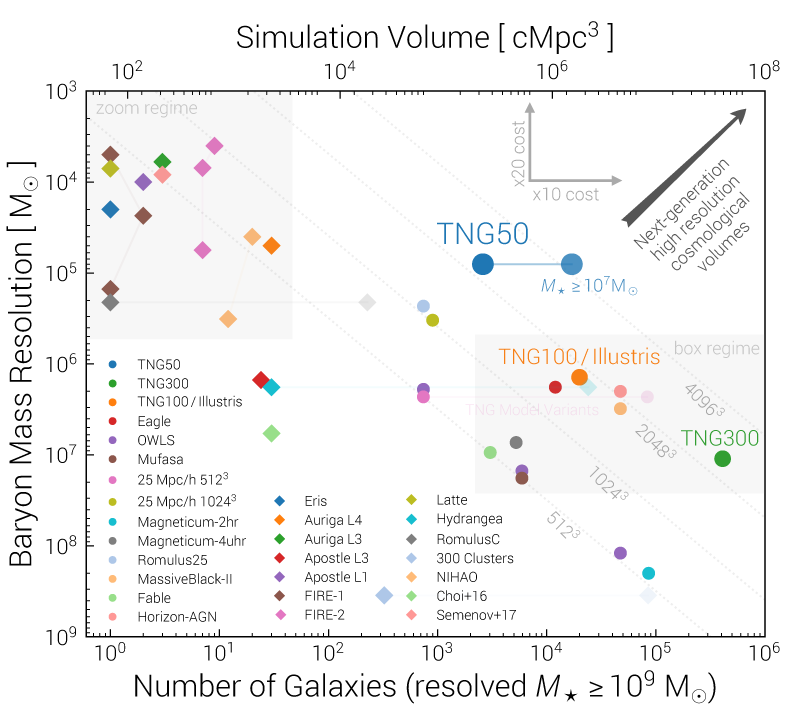
\includegraphics[width = \linewidth]{Figures/Chapter2/VolumeResolutionComparison.png}
    \caption{In this figure the positions of several simulation is volume-resolution space is shown. The vertical axis is baryon mass resolution or the size of the elements in the simulation. The horizontal axis is the simulation volume (shown on the top) which correlates with the number of galaxies (shown on the bottom). The faint grey lines running from top left to bottom right are lines of constant particle number. The two shaded boxes in the top left and bottom right show respectively the zoom and box simulation regimes. Coloured shapes are galaxy simulations as labelled. 
    Image used with permission from: Illustris-TNG Project, \citet{Nelson2019FirstFeedback}}
    \label{fig:Vol_v_Res}
\end{figure}

Semi-Analytic and Semi-Empirical models are also constrained by volume and resolution in a simmilar way. Traditionally each uses merger trees which can either be generated analytically or extracted from an N-body simulation, r
for those models that use N-body simulations directly they have simmilar constraints as in Figure \ref{fig:Vol_v_Res} but with dark matter particle resolution and number of haloes. Simply, the number of haloes on a given merger tree is directly related to the lowest mass halo of interest. However, models using merger trees have one additional level of flexibility: they can have a minimum subhalo mass and a minimum central halo mass. This provides flexibility in what can be simulated, by flexibly `pruning' the tree and removing (sub)haloes we can adapt the halo background we are using to focus computational power on important features. 

\steel has been specifically designed to overcome the limitations of volume and mass resolutions using a \textit{``Statistical Dark Matter Accretion history''} described in full in Section \ref{subsec:SDMAH}. In brief, the statistical accretion histories follow the average growth of a given mass of halo backwards in time from $z = 0$. At each time-step, t, the average number of infalling subhaloes to a given halo growth history is calculated by comparing the USHMF at t and t +$\Delta$t. The lifetime of subhaloes controlled by the input dynamical timescales. The advantage of calculating the subhalo accretion in this way is that the prerequisites are only the average halo mass growth and the USHMF, each of which have been analytically defined \cite{vandenBosch2014ComingWells, Jiang2016StatisticsFunctions}.
\steel therefore simulates massive haloes and small haloes on equal footing and is able to produce massive rare galaxies in the same run as smaller galaxies with the same precision.

\subsection{Flexibility through stability}
%Flexibility - empirical
Hydrodynamical and Semi-Analytic models are tuned for two reasons. The first is for stability, these models have tens of parameters acting in the sub-grid for hydrodynamical or as the primary modelling tool for semi-analytic models. The issue stems from multiple parameters each contributing to one galaxy variable, changing one parameter ripples throughout the model. In abstract consider a model with two parameters, $\alpha$ that controls a galaxy mass with a secondary effect on size, and $\beta$ that controls galaxy colour with a secondary effect on galaxy mass. Changing $\beta$ with the intent of modifying the colour of galaxies will force a reaction in $\alpha$ to compensate for the change in mass and then propagate into the size of galaxies. Secondly, the tuning allows fits to observations, the models are given freedom in their parameter sets to fit many galaxy properties at the same time but due to the overlap in what each physical assumption can control this leads to degeneracy in parameter space. To complicate comparison further, some models have more physical routines than others resulting in models and parameters in the less complex model compensating for this missing physics. The diversity in models and the diversity introduced by different tuning data has been extensively discussed in the literature \cite{Knebe2015NIFTyModels,Cui2018TheApplications,Knebe2018CosmicModels}.   

This degeneracy has in some part been addressed by semi-empirical models. Fundamental variables, such as galaxy stellar mass, are set using observationally-based techniques such as abundance matching (Section \ref{C2:SubSec:AbnMtch}), which remove the reliance on the physical models and parameters that are required to generate this quantity in more comprehensive/ab-initio models. `Bottom-up' modelling like this gives semi-empirical models the ability to use dramatically reduced parameter spaces and also reproduce essential observables, such as the central stellar mass function, by design. Additional physical models are added only where necessary, creating tight constraints for the core of the model and severely limiting possible degeneracies. In the semi-empirical framework, additional physical processes and associated parameters can be added in a modular fashion. For example, \citet{Shankar2014} added an analytic recipe for the size evolution of galaxies onto a network of dark matter merger trees in which central and satellite galaxies were assigned via abundance matching techniques. In the \citet{Shankar2014} SEM, the addition of the ``size evolution'' block, is completely independent of the core features of the model, namely the mass evolution of galaxies, which is fully controlled by the dark matter assembly and the input SMHM relation. This modularity of SEMs prevents degeneracies which often affect more complex, multi-parameter models. Semi-empirical models can use this to great advantage testing, for example, multiple size evolution models on one assembly background without need for re-tuning or fear of disrupting the essential results. In this thesis we extend this idea of empirical stability and flexibility further. In STEEL the backbone is of statistical nature, in which the different additional physical processes are expressed in the form of probabilistic models. These models are entirely modular and their impact on the final outputs can be individually analysed. 

It is noteworthy that some hydrodynamical cluster simulations are beginning to use a technique where haloes/galaxies are ``genetically modified''. This methods runs a simulation multiple times and making slight adjustments to the initial conditions such that the models are nearly identical aside from, for example, changing the distribution of dark matter to preference a larger merger mass ratio without changing the total simulation mass. This is a highly complementary and powerful technique that is yet to be fully realised \cite{Rey2018QuadraticHistory}.

\subsection{Consistency}
%Consistency - ensuring connections between high and low redshift
It is well documented that reproduction of the stellar mass function as multiple epochs has been a challenge for semi-analytic models \cite{Knebe2018CosmicModels, Asquith2018CosmicModels} and hydrodynamical models (although major improvements have been seen recently, for example, Illustris vs Illustris TNG \cite{Nelson2015TheRelease, Nelson2019TheRelease}). This has not however prevented such models from making bold claims about the successes of their models in terms of morphology and mass assembly without providing a full stellar mass function history \cite[e.g.][]{Somerville2008ANuclei, Hopkins2010MERGERSMATTER}\footnote{A merger history matched to an observational merger history as provided by \citet{Hopkins2010MERGERSMATTER} is insufficient as we show in Chapter \ref{Chapter:GalPairs} the methods involving pair fractions used to estimate these rates have a large degree of systematic error.}. However, it is the opinion held by PJG that these claims should be viewed as entirely unsubstantiated. As an example, if a kettle at temperature A that is modelled to cool under an arbitrary physical model $\gamma$ to temperature B in time T. If A is observed to be false compared to the data and B is observed to be consistent with the data than the inference that $\gamma$ is a correct physical model is baseless. Galaxy models that fail to reproduce the stellar mass function at high redshift repeatedly invoke this kind of logic when the $z=0$ stellar mass function is reproduced. An overabundant stellar mass function at high redshift that evolves to the observed stellar mass function at low redshift implies either lack of growth in the galaxy population to allow the observed stellar mass function to catch up or over merging of galaxies to reduce the total number density.

A semi-empirical model that puts reproduction of the stellar mass function and the distribution of satellite galaxies as the foremost modelling priority has a major advantage. Any internally self-consistent model is a viable candidate for the true physical model with stronger evidence than those presented in models that do not achieve consistency over multiple epochs. 

\subsection{Speed}
%Systematics - speed

Speed is a critical ingredient to any model, hydrodynamic models have run-times of months using millions of CPU hours, and semi-analytic models constrain highly-multi dimensional parameter space for thousands of merger histories. In each case speed allows for the models to reach conclusions in shorter time frames. Semi-empirical models are faster by design with smaller better-constrained parameter spaces, they can therefore leverage more computational time to explore physical models or larger simulation boxes. In forgoing discrete merger trees the run time of \steel depends on different factors to other models, the width of the mass bins used for the halo and subhalo mass functions (which corresponds to the resolution of halo or mass particle) and secondly is the computational complexity of any physical modelling routines. Where \steel is not running to tune to high N parameter space or thousands of discrete merger trees it can instead test combinations of internal physical models or be run on more modest, cheaper, and widely accessible hardware.

\section{Modules and Methods}

\subsection{Statistical Dark Matter Accretion History}
\label{subsec:SDMAH}

Fundamentally, the single most important element of \steel and a large part of what makes it unique enabling an alternative view of galaxy formation problems is the \textbf{\textit{statistical dark matter accretion history}}. As described above a large part of the power of \steel come from the removal of discrete merger tress or haloes achieved using this technique. We provide here a discussion of n-body and processed merger trees building upon Section \label{sec:LCDM} followed by a detailed description of how the statistical dark matter accretion history is constructed.

%First we should explain merger trees and traditional simulation techniques.
\subsubsection{Traditional methods and merger trees}

%first n body

The state of the art in dark matter modelling is n-body simulations, simulating billions of individual particles and solving the equation of state for each over many epochs to simulate their evolution from the distributions calculated from the CMB to the cosmic web of haloes and filaments inferred from observations of galaxies today. The non-interacting nature of \textbf{cold} dark matter is extremely fortuitous as it means its behaviour can be modelled using gravitational tensors only thus modern dark matter simulations are able to leverage the massive power gains made recently in GPU computing allowing for ever larger and higher resolution dark matter only simulations to be run. 

Whilst the massive n-body simulations are impressive they do little to impact our understanding of galactic astrophysics, the outputs of even the previous generation n-body dark matter simulations such as the Bolshoi simulation a snapshot of which is shown in Figure \ref{fig:Bolshoi} total tens of gigabytes for individual sections and terabytes to capture the whole simulation. To use all of this information would be impractical for any galactic modeller without access to high-performance computing hardware and a good understanding of memory management. Furthermore, despite the excellence provided by halo-finders and merger tree extractors such as \textsc{rockstar} \cite{Behroozi2011TheCores} and the `consistent trees' algorithm \cite{Behroozi2013GRAVITATIONALLYCOSMOLOGY}, the merger trees are frequently not fit for use in models unless specifically built to handle these inputs. Finally, as discussed by van den Bosch \cite{vandenBosch2014ComingWells, vandenBosch2017DissectingSimulation, vandenBosch2018DisruptionFiction} the interpretation of dark matter simulations is of vital importance, as the analysis tool and the fundamental design decisions taken in building the simulation all have systematic effects on the outputs all of which complicate comparison between simulation.

\begin{figure}[h]
    \centering
    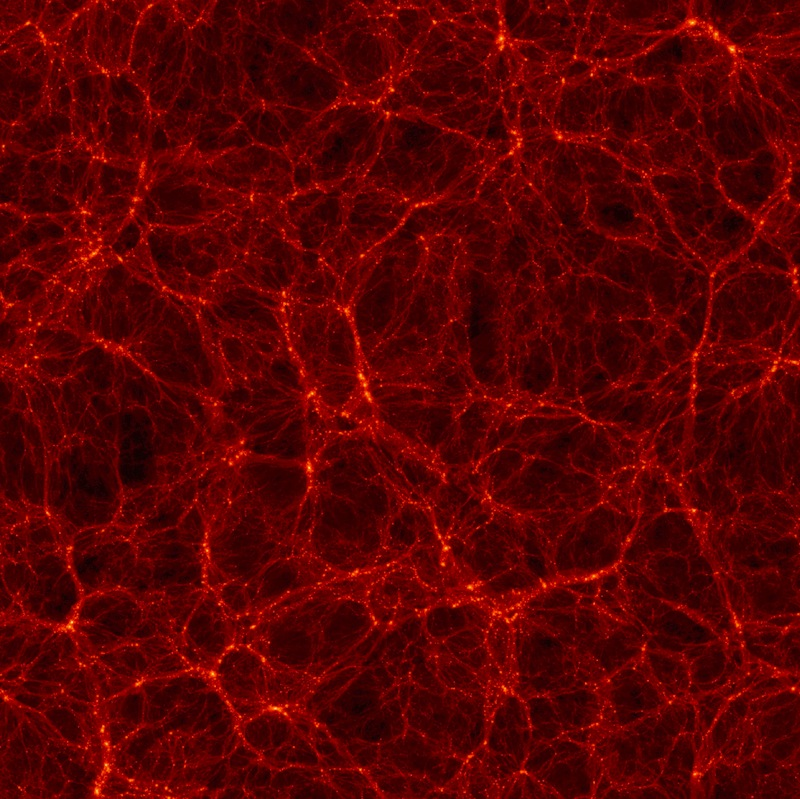
\includegraphics[width = \linewidth]{Figures/Chapter2/Bolshoi.jpg}
    \caption{Snapshot of the 250 Mpc$^3$ box of the Bolshoi Simulation. Brighter regions indicate a higher density of dark matter. Note the clustered bright points connected by large filaments. This structure is known as the cosmic web.
    Image credit: Bolshoi Simulation http://hipacc.ucsc.edu/Bolshoi/Images.html}
    \label{fig:Bolshoi}
\end{figure}

The choice of many analytic and empirical models to instead opt for analytically derived Press Schecter trees that can be generated 'on-the-fly' or pre-processed comes from the simplicity and flexibility afforded by this technique. However, trees generated in this way are still affected by volume (i.e. number simulated) and resolution (i.e. size of the smallest halo accounted for in any split) limiting there effectiveness.

\subsubsection{State of the art statistical method}
%then get onto what makes STEEL STEEL
\begin{figure}[h!]
    \centering
    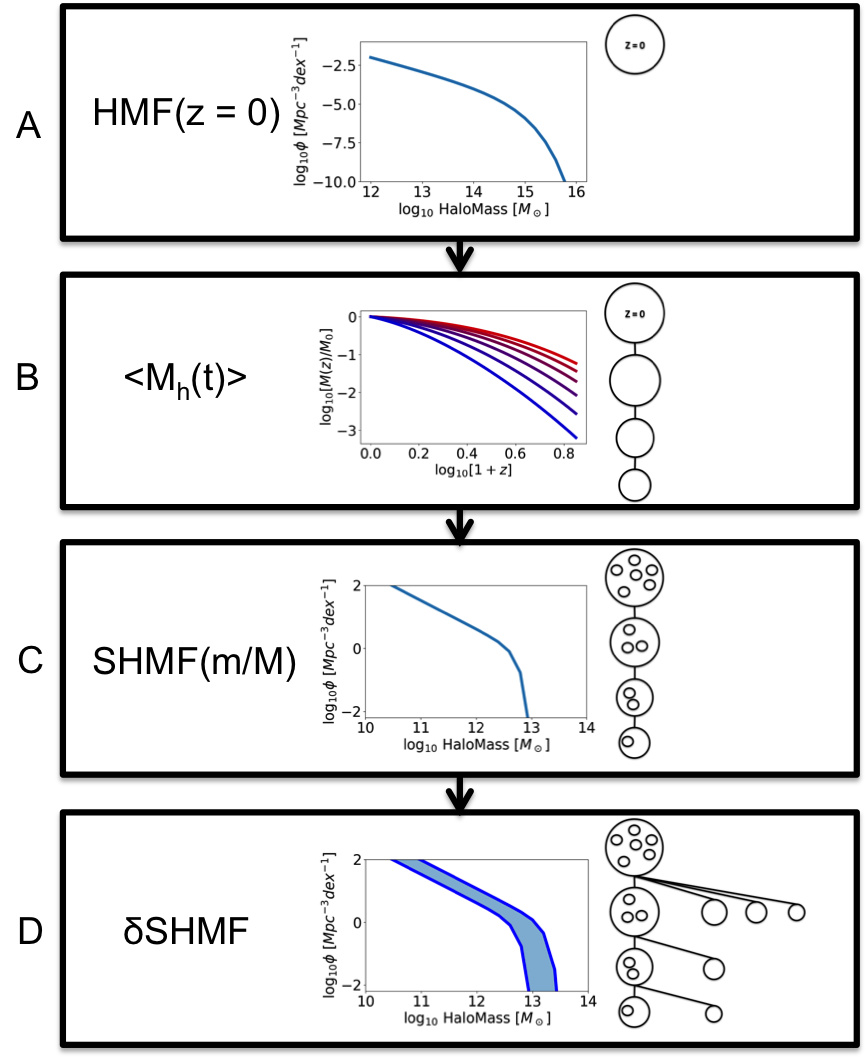
\includegraphics[width = \linewidth]{Figures/Chapter2/StatDM.png}
    \caption{We show the main steps in building the statistical dark matter accretion history for STEEL. Each panel shows a feature from a traditional merger tree and the statistical function used to replace it. A: The HMF is used to calculate the number densities of central haloes. B: Average mass growth histories are used to calculate the size of each mass bin at previous epochs. C: The (unevolved)SHMF is used to populate each central at each redshift with subhaloes. D: The average number densities of accreted subhaloes at each epoch are calculated by taking the difference between each mass bin of the (unevolved)SHMF at consecutive redshift steps.}
    \label{fig:StatDM}
\end{figure}

The core principle of the statistical methodology is to treat parent haloes, and satellites galaxies/haloes, as ``average'' populations avoiding the issues with volume and resolution as described previously. Here we detail step by step construction of the statistical dark matter accretion history complemented with a graphic representation in Figure \ref{fig:StatDM}.

\textbf{Central Haloes}

We start by considering a fine grid of central dark matter haloes ranging from $M_{h}=10^{11}\, M_{\odot}$ to $M_{h}=10^{15}\, M_{\odot}$ at redshift $z=0$. Their number densities are given by the halo mass function (HMF) of \citet{Despali2016TheDefinitions}, which is obtained using the COLOSSUS Python package \citep{Diemer2018COLOSSUS:Halos} which contains many other halo mass functions as well as spherical over-density conversions required throughout this work.

The halo mass function provides the number of densities of haloes in a given mass bin (Figure \ref{fig:StatDM}, Panel A).
The average mass growth histories of all main progenitors with mass in the bin of halo mass $[M_{h},M_{h}+dM_{h}]$, are then calculated using the analytic model from \cite{vandenBosch2014ComingWells}\footnote{This model further improves on the seminal work by \citet{Parkinson2008GeneratingTrees}, which was aimed at reproducing numerical merger trees, optimised with small redshift steps minimising the development of systematic errors at late cosmic epochs.}. This provides the average ``main progenitor'' branch of a traditional merger tree for each mass bin at $z = 0$ (Figure \ref{fig:StatDM}, Panel B.)

\textbf{Assigning Subhaloes to Parent Haloes}

In order to predict the number of satellite galaxies, we must associate to each parent/central halo the number and mass of subhaloes they are expected to contain. To achieve this we use the subhalo mass function (SHMF). The SHMF describes the expected distribution of subhaloes, of mass $M_{h,sat}$, in a given parent halo of mass $M_{h,cent}$, as a function of $M_{h,sat}/M_{h,cent}$. Multiple definitions for the SHMF exist depending on the way a subhalo is defined. In this work we use two definitions of the SHMF. The first is the unevolved SHMF (USHMF), which describes the total subhaloes accreted over a parent halo's lifetime. In the unevolved SHMF any merging or stripping in the subhaloes occurring after infall is ignored. Several groups have been able to constrain the unevolved SHMF \citep{Giocoli2008AnalyticalHaloes,Jiang2016StatisticsFunctions}. In what follows, we use a recent rendition of the unevolved SHMF by \citet{Jiang2016StatisticsFunctions}, which is calibrated against the Bolshoi simulation\footnote{We direct the interested reader to \citet{Jiang2016StatisticsFunctions} for further discussion of the unevolved SHMF as well as of other SHMFs, such as the evolved SHMF where the number densities are affected by both subhalo stripping and mergers.}.

The second definition we use in this work is the unevolved ``surviving'' SHMF (USSHMF). Subhalo masses are assumed frozen at infall but the subhalo number densities can reduce compared to the unevolved SHMF as the unevolved surviving SHMF accounts for subhalo disappearance due to merging with the parent halo. Sub-halo merging is due to loos of angular momentum to the parent halo via `Dynamical Friction' described in Section \ref{subsub:DynF}. We show in Figure \ref{fig:SHMF_clus} for a representative parent halo of mass $\log M_{h,cent} M_{\odot} = 12.80$, the unevolved SHMF and three unevolved surviving SHMF characterised by different dynamical friction timescales $\tau_{dyn}$. Larger $\tau_{dyn}$ lead to a milder reduction in subhalo number densities as subhaloes take longer to merge with the parent halo. Lower $\tau_{dyn}$ are less effective in reducing the number densities of smaller subhaloes which are more likely to have dynamical friction timescales comparable to or larger than the Hubble time at $z = 0$.
\begin{figure}[h!]
    \centering
    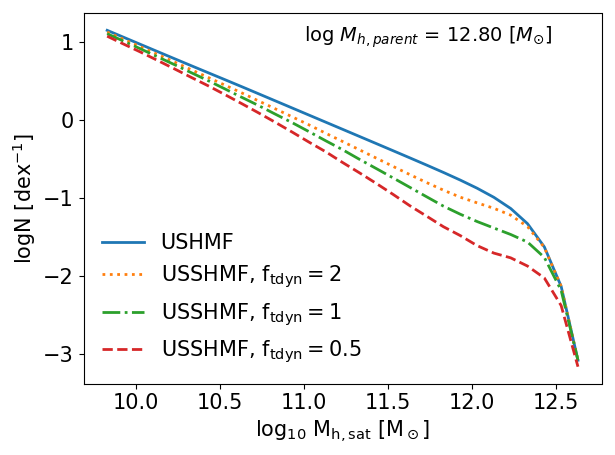
\includegraphics[width = \linewidth]{Figures/Chapter2/SHMF_OneCluster.png}
    \caption{Comparison between the unevolved SHMF (solid line) and three unevolved surviving SHMF  (dotted lines) for a parent halo of mass $\log$ $M_{h,parent}$ $[M_{\odot}] = 12.80$. The factor $f_{t_{dyn}}$ is applied to the merging timescales of the haloes. Lower factors correspond to lower unevolved surviving SHMF where more sub haloes have merged.}
    \label{fig:SHMF_clus}
\end{figure}

\textbf{Average Subhalo Accretion}

At each redshift step along with the mass growth histories, we calculate the unevolved SHMF associated to the parent halo mass. This is equivalent to the substructure found in traditional merger trees (Figure \ref{fig:StatDM}, Panel C). However, unlike traditional methods, our statistical approach is able to probe ``rare'' subhaloes without running prohibitively large volumes of merger trees.

For each time step we can now calculate a mass function describing the number density of subhaloes accreted onto the population of central haloes in the halo mass bin $[M_{h,cent}(z),$ $M_{h,cent}(z) + dM_{h,cent}(z)]$. The latter is achieved by differentiating the unevolved SHMF across two neighbouring redshift steps $z$ and $z+dz$, we can calculate the average number density of subhaloes of any given mass $M_{h, sat}$ that are accreted in the redshift interval $dz$ onto the main progenitor haloes with mass in the bin $[M_{h,cent}(z),$ $M_{h,cent}(z) + dM_{h,cent}(z)]$,
\begin{equation}
\label{eqn:deltSHMF}
\begin{split}
&\delta USHMF[z, M_{h,cent},M_{h,sat}] =  \\
&USHMF\Big(\frac{M_{h,sat}}{M_{h,cent}(z)}\Big) - USHMF\Big(\frac{M_{h,sat}}{M_{h,cent}(z + \delta z)}\Big)
\end{split}
\end{equation}
In this way the unevolved subhalo accretion history ($\delta USHMF$) is retrieved for all main progenitor haloes at all redshifts.

\subsubsection{Dynamical Friction}
\label{subsub:DynF}
Dynamical Friction is the process by which an object (particle) moving though a mass `field' (or distribution of particles) looses velocity and increases the velocity of the field via gravitational interactions. A simplified example is shown in Figure \ref{fig:Tdyn_toon}, the red particle is initially moving to the left between two rows of particles of infinite extent that interact only though gravity (and only with the red particle). The particle in Panel A receives an equal pull from all particles and therefore experiences no acceleration the black particles directly above and below the red are the most strongly attracted and therefore move the greatest distance toward the red, with further particle moving slightly less. By Panel B the red particle has moved to the left and due to the previous effects now has more clustered mass directly behind it path. The break in the symmetry act to exert a net force on the red particle in the opposite direction to its motion. The black particles nearest the red are again drawn toward it most and after the red particle has moved further to the left again in Panel C the effect is magnified with the number of particles directly behind and the resultant force strongly opposes the motion. 

\begin{figure}[h!]
    \centering
    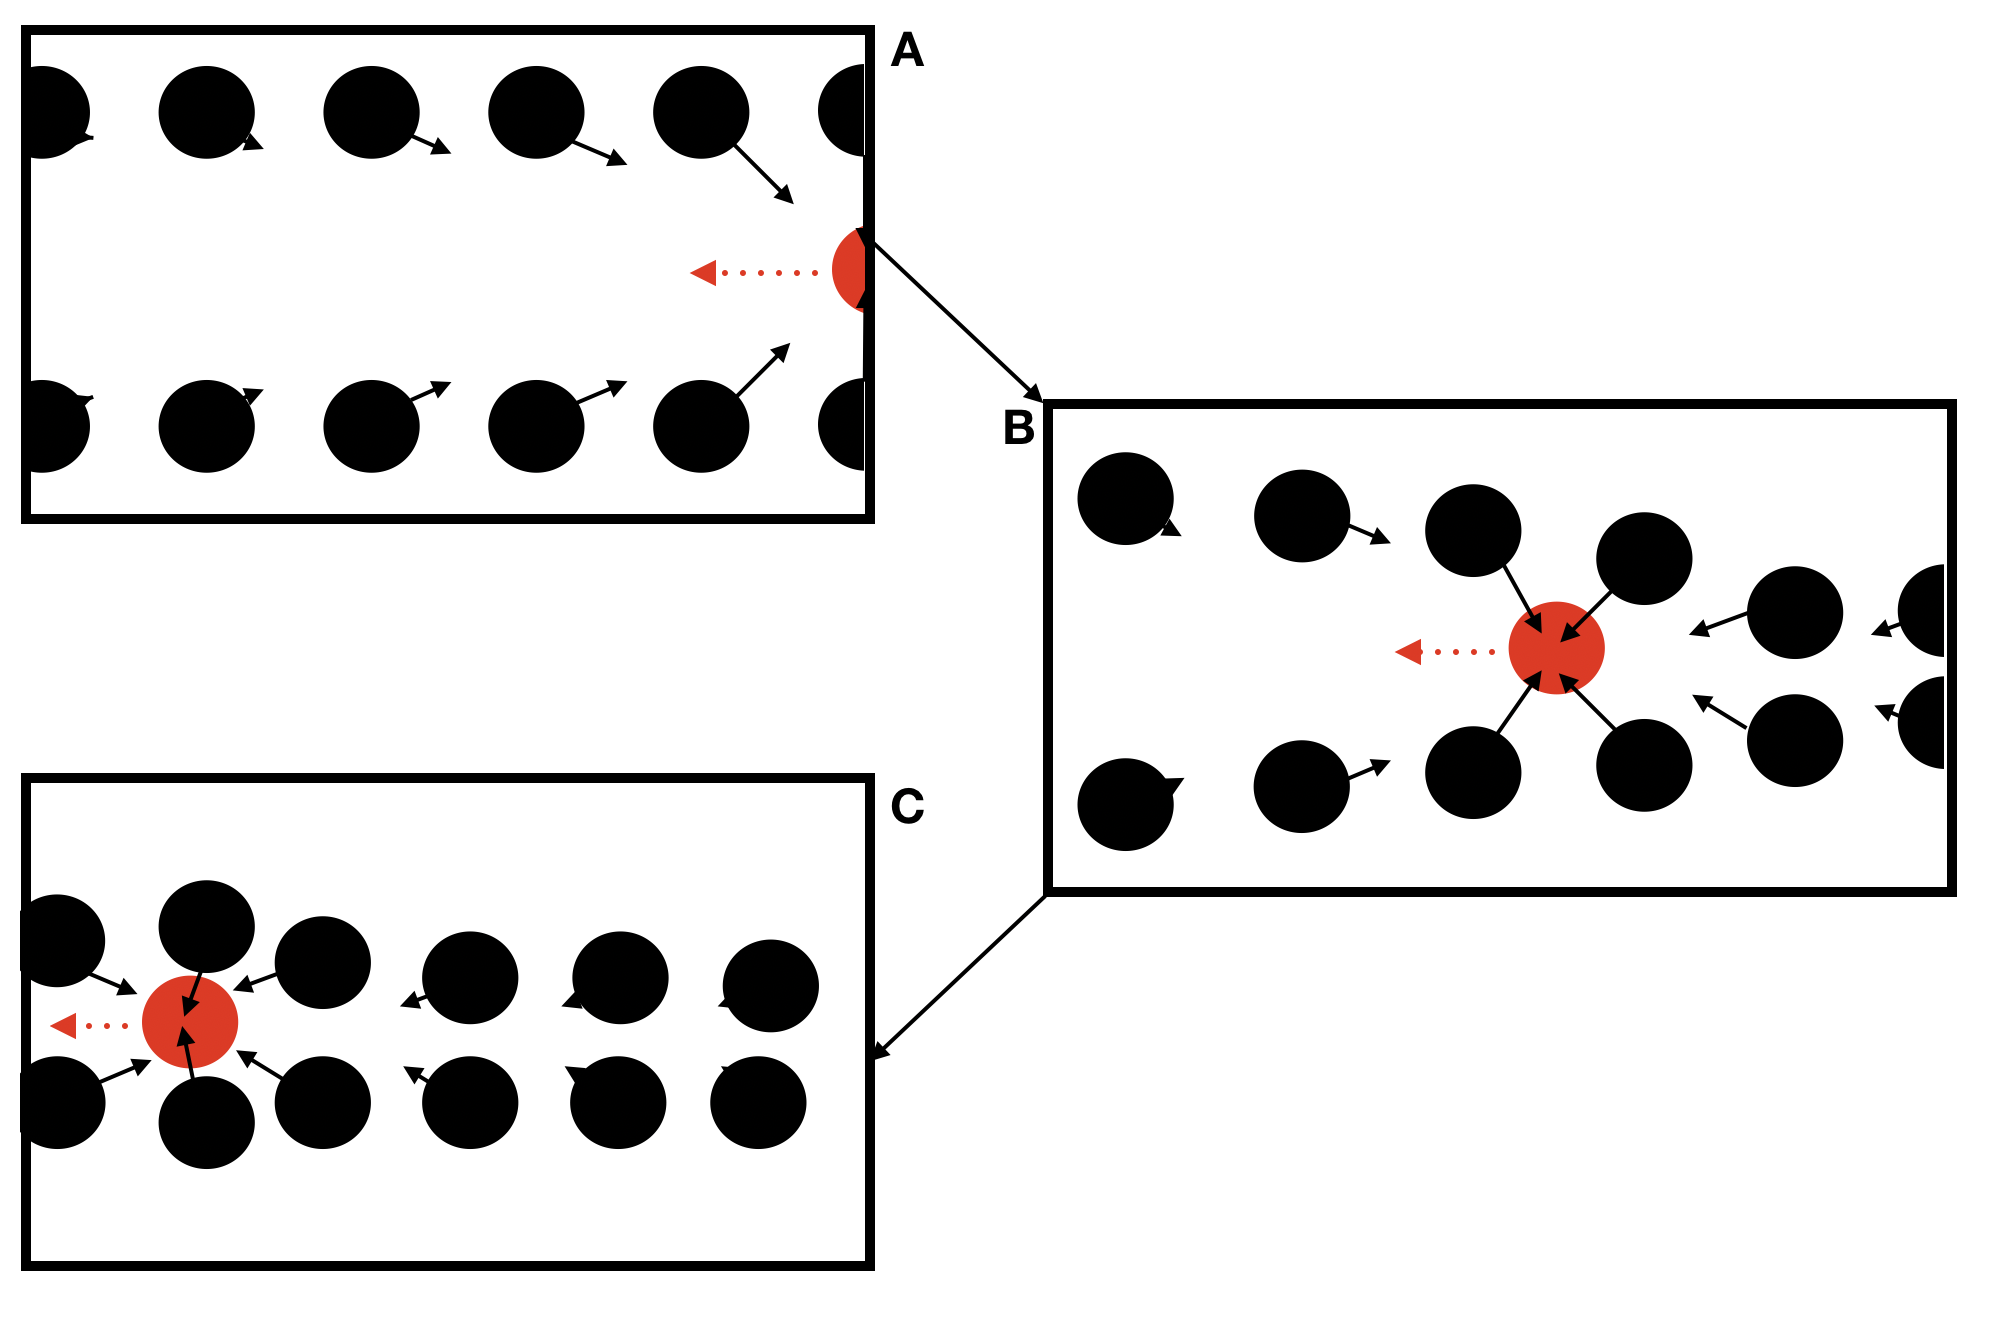
\includegraphics[width = \linewidth]{Figures/Chapter2/Dynamical_Friction.png}
    \caption{In this hand made cartoon, we depict a thought experiment to demonstrate the process of dynamical friction. We show a red test particle moving though two rows of black particles that are infinite in extent. The particles interact only though an attractive force that reduces with distance akin to gravity. The black particles interact only with the red and not with each other. The black particles start at rest and the red particle starts with some arbitrary velocity to the left. The panel A shows the starting configuration of the particles, the panels B and C show two theorised later states of the system. For an animation of a simulation designed around this thought experiment see: \url{https://twitter.com/RSEGrylls/status/1229104848643198979} (made and shared by PJG)}
    \label{fig:Tdyn_toon}
\end{figure}

As a descriptive thought experiment this case achieves several of the properties dynamical friction has well:
\begin{itemize}
    \item The red particle experiences a `drag' force due to the particles it draws in behind it, eventually loosing most of its momentum.
    \item The particles are non-interacting aside from gravity, as are the leading dark matter theories.
    \item The energy of the red particle is dissipated into the velocities of the black particles, the motion of a galaxy though a dark matter field increase the random motion of the dark matter.
\end{itemize}
The main features missing from the thought experiment are:
\begin{itemize}
    \item The dark matter field is not uniform and in-fact are a virialised potential well with more mass in the centre and the distributions and velocities of particles within this field are random within this distribution.
    \item The red `test' particle is in-fact a distribution of masses that are gradually lost to the field.
    \item The red particle moves in an orbit around the centre of the potential well and is stripped of mass, velocity, and momentum.
    \item The dark matter is self interacting under gravity and there is baryonic matter that interacts via processes other than gravity, although these tend to be of a lower order.
\end{itemize}



\section{Utilised Data}

In this thesis we use the stellar mass functions defined below, along with the halo mass functions, to constrain the SMHM relationship. In addition to the SMF to constrain the model at high redshifts we use measurements of massive clusters to constrain the satellite galaxy distributions.

\subsection{Stellar Mass Functions}
\label{subsec:SMF}

\subsubsection{Low Redshift, $z = 0.1$}
\label{subsub:SDSS}
At low redshift we use the Sloan Digital Sky Survey Data Release 7 (SDSS-DR7) from \citet{Meert2015ASystematics}.
The data from the SDSS-DR7 spectroscopic sample \citep{Abazajian2009THESURVEY} contain $\sim 670,000$ galaxies fitted with a S\'ersic + exponential model \citep[PyMorph;][]{Meert2015ASystematics} with associated halo masses and central satellite classifications from \citep{Yang2012EvolutionHalos}. The improved photometric analysis by \citet{Meert2015ASystematics} provides more reliable estimates of the stellar mass function at the high mass end which are more abundant than previous estimates \citep{Bernardi2016TheEvolution, Bernardi2017ComparingLight}.
In this thesis the effect of the enhanced high mass end on galaxy assembly is investigated. We compare to previous determinations of the stellar mass function using as an example the de Vaucoulers \citep{deVaucouleurs1948RecherchesExtragalactiques} based cmodel fits from SDSS \citep{Abazajian2009THESURVEY}. The latter definition of galaxy stellar mass has been extensively discussed not to be accurate, partially due to incorrect sky subtraction and adoption of non-ideal light profiles \citep{Bernardi2013TheProfile}. \citet{Bernardi2017ComparingLight} have clearly shown that the choice of light profile is not a simple matter of ``semantics''. The single or double S\`ersic models perform better in fitting the surface brightness of galaxies independently of the galactic environment \citep{Meert2015ASystematics}. The performance is thus not related to the inclusion of the intra-group or intra-cluster light in the fit \citep{Bernardi2017ComparingLight}.

\subsubsection{High Redshift, $z > 0.1$}
\label{subsub:Davidzon}
At higher redshift (0.3 \textless z \textless 3.3) we use stellar mass functions from the COSMOS2015 catalogue \citep{Davidzon2017TheSnapshots}. Here masses are defined using spectral energy distribution fitting, including ultra-deep infrared photometry. \citet{Davidzon2017TheSnapshots} use \citet{Bruzual2003Stellar2003} stellar population synthesis models to estimate stellar masses. As SED fitting is notably different from light profile fitting, one cannot apply the same corrections as in \citet{Mendel2014ASURVEY}. 
Nevertheless, to match the mass-to-light ratios adopted by \citet{Mendel2014ASURVEY}, based on the \citet{Bell2003TheFunctions} mass-to-light ratios, we follow \citet{Bernardi2013TheProfile} and increase the \citet{Davidzon2017TheSnapshots} stellar masses, based on \citet{Bruzual2003Stellar2003}, by +0.15 dex. We note that the resulting $z=0.37$ stellar mass function after this correction is in remarkable good agreement with the $z=0.1$ stellar mass function by \citep{Bernardi2013TheProfile}. Our result also matches the findings by \citet{Bernardi2016TheEvolution}, who showed that, by making use of the BOSS sample, the stellar mass function shows negligible number density evolution up to $z \sim 0.5$.

\label{subsec:Clusters}
\subsubsection{Cluster at z = 2.5, Wang+ 2016}
\label{subsubsec:Wang}
The highest redshift cluster we compare to is a $M_{vir} = 10^{13.7} M_{\odot}$ halo containing 15 galaxies with $M_* > 10^{10} M_{\odot}$ at a redshift of $z = 2.5$.
This cluster is reported in \citet{Wang2016DISCOVERY2.506}, and we provide a brief description of the observation and data here.
The cluster is observed using IRAM-NOEMA, VLT-KMOS, VLA, XMM-Newton and Chandra for the spectroscopic observation and redshift determination.  
The galaxy masses are determined assuming a \citet{Salpeter1955TheEvolution.} IMF, which we correct to a \citet{Chabrier2003GalacticFunction} IMF, by decreasing the stellar masses by 0.24 dex.
The halo mass ($M_{vir} \sim 10^{13.93} M_{\odot}$) of the cluster is estimated in three different ways, using the total X-ray luminosity, the velocity dispersion of its member galaxies above $M_* = 10^{10.76} M_{\odot}$, and the stellar richness of the cluster \footnote{We note the velocity dispersions and X-ray luminosity estimations give the cluster mass as $M_{vir} = 10^{13.73} M_{\odot}$ and the estimate given by mass richness is significantly higher $M_{vir} = 10^{14.6} M_{\odot}$, whilst we used the published average the lower cluster mass excluding the richness estimate is in as-good or better agreement with model results.}. Given this object was a targeted cluster, we cannot estimate the cosmic abundance (i.e, the number per cubic megaparsec). For analysis and comparison later in this work we assign this cluster an abundance of $N(> M_*=10^{13.93})=10^{-7.15}$ $[Mpc^{-3}]$ which is estimated by integrating the halo mass function in the limits [$10^{13.93}$, $\infty$], thus providing an upper limit to the number densities associated to clusters of this mass. 

\subsubsection{1959 Clusters at z = 0.7 - 1.0, Wen \& Han 2018}
\label{subsubsec:1959}
We compare to the cluster sample from \citet{Wen2018ARedshifts}, which contains 1959 clusters from SDSS-DR14 \citep{Abolfathi2017TheExperiment} and the WISE survey \citep{Wright2010THEPERFORMANCE}. The clusters are identified in the W1 band, and foreground objects are removed using the SDSS photometric data. The cluster mass and richness are estimated using the total W1 band luminosity within 1 Mpc of the central galaxy. As performed above, to each cluster we assign an upper limit to their abundances from the cumulative integration of the halo mass function.

\subsection{Abundance matching}
\label{C2:SubSec:AbnMtch}
In this work we populate dark matter haloes with galaxies using the abundance matching technique where galaxies are assigned to haloes by comparing the relative abundances of galaxies and haloes. For example in Figure \ref{fig:Abn_Toon} the horizontal lines connect points of constant number density between the HMF (red, top left) and the SMF (green, bottom right). Halo/stellar masses with corresponding number density are then used to define a mapping between the masses, this connection is called the stellar-mass-halo-mass (SMHM) relationship (black, bottom left).

\begin{figure}[h]
    \centering
    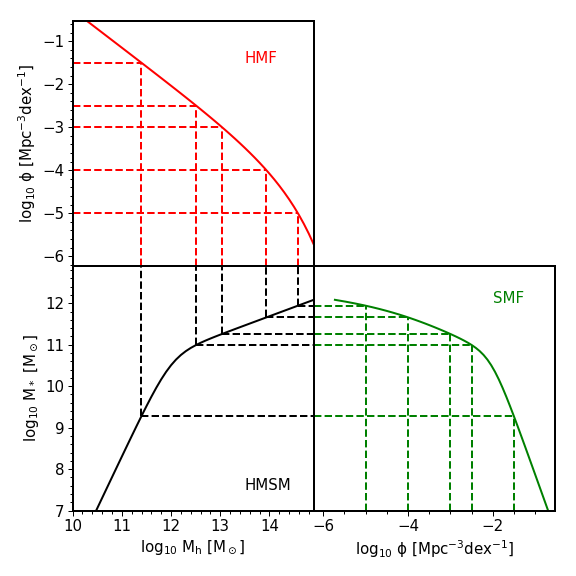
\includegraphics[width = \linewidth]{Figures/Chapter2/AbundaceMatching.png}
    \caption{A cartoon to show by matching the HMF (top left) and the SMF (bottom right) by abundance and the mapping between stellar and halo mass referred to as a SMHM relation (bottom left) is created.}
    \label{fig:Abn_Toon}
\end{figure}

The abundance matching used in \steel extracts central haloes from the halo mass function from \citet{Despali2016TheDefinitions} obtained using \textsc{colossus}\cite{Diemer2018COLOSSUS:Halos}, and a subhalo mass function subdivided by the redshift of infall generated from the statistical dark matter accretion history used by \textsc{steel}. Sub-haloes are assumed to follow the central SMHM relation at infall. We simplify our abundance matching by using a frozen model such that baryonic evolution after infall (stripping, star formation, etc.) is not included. The latter assumption provides a good approximation as after infall the dominant factor determining the abundances of satellite galaxies is the dynamical time and not evolutionary processes (Paper \RomanNumeralCaps{1}).

To fit stellar mass functions over multiple epochs we convolve our halo mass functions with a parametric SMHM relation similar to that proposed by \cite{Moster2010},
\begin{equation}
\label{eqn:MosAbn}
\begin{split}
M_*(M_h, z) &= 2M_hN(z)\Big[ \Big( \frac{M_h}{M_{n}(z)}\Big) ^{- \beta(z)} + \Big( \frac{M_h}{M_{n}(z)}\Big)^{\gamma(z)} \Big ]^{-1}\\
N(z) &= N_{0.1} +N_z\Big(\frac{z-0.1}{z+1}\Big)\\
M_{n}(z) &= M_{n,0.1} +M_{n,z}\Big(\frac{z-0.1}{z+1}\Big)\\
\beta(z) &= \beta_{0.1} +\beta_z\Big(\frac{z-0.1}{z+1}\Big)\\
\gamma(z) &= \gamma_{0.1} +\gamma_z\Big(\frac{z-0.1}{z+1}\Big).
\end{split}
\end{equation}

In what follows we create SMHM relations using both the cmodel and PyMorph SMF described in Section \ref{subsec:SMF} at redshift $z=0$ to constrain the parameters N, M, $\beta$, and $\gamma$ (normalization, knee, low mass slope, and high mass slope). We use only the central stellar mass function, using the \cite{Yang2012EvolutionHalos} central/satellite identification, and central halo mass function. The fit is performed using a Markov Chain Monte Carlo (MCMC)\footnote{In actuality the fit is first done by hand correcting parameters one at a time and visualised at each step. In doing so an appreciation of the connection between parameter value, SMHM shape, and SMF is built that promotes an in-depth understanding of the system and its caveats. Around the minimum value a brute force search is performed with various ranges and resolutions, this provides a test of the fit estimator that will be included in the MCMC. Once the limitations of the method are known building the MCMC is more robust as sensible checks and balances are included. The MCMC will often provide a solution close to the one found by the previous methods but find the robustness/errors associated with the result.}, implemented using the \textsc{python} package \textsc{emcee} \citep{Foreman-Mackey2013EmceeHammer}, over a large parameter space ($P_{M, N, \beta, \gamma}$) covering all four parameters. Given a point in parameter space $P_{M_i, N_i, \beta_i, \gamma_i}$, the stellar mass function is constructed using the halo mass function and the SMHM relation. Each bin of the central halo mass function is associated with a Gaussian distribution of stellar mass via the SMHM relation with scatter 0.15 dex. This distribution is multiplied by the halo mass number density to convert to galaxy number density which is added to the relevant stellar mass bins of the stellar mass function in construction. This operation is then repeated overall mass bins of the halo mass function to produce the complete central stellar mass function. For each point, $P_{M_i, N_i, \beta_i, \gamma_i}$ in the parameter space, the stellar mass function associated to that point is compared via a likelihood function to the observed stellar mass function to provide the MCMC with the probability that the given point is the `true' SMHM relationship. 

In Figure \ref{fig:Gauss_build} the above process is visualised, stripes in halo mass function are selected as shown in the left hand plot and then again in the middle as red bands. By propagating these bins of halo mass through the SMHM relation and associated scatter they each create a Gaussian of stellar mass as shown by overlapping green shading in the middle panel. Once weighted by the median halo number density they are added as green solid lines in the rightmost panel. Summing up each of the Gaussians created an estimation of the stellar mass is achieved. This figure is available animated at \url{https://twitter.com/RSEGrylls/status/1231279549704474624}. From this figure we see several features of the SMHM relation:
\begin{itemize}
    \item From the visualisation it can be seen that the scatter in the SMHM relation has two major effects: Firstly it can smooth out jaggedness introduced by the binning, one should therefore ensure that the scatter parameter is not influenced by the size of the binning to ensure results are physical and not numerical artefacts; Secondly the scatter dictates the size of the stellar mass gaussians it therefore dictates the range of stellar masses within a given halo mass bin. The width of the scatter has a second effect whereby lower mass halo bins can contribute to higher mass stellar mass bins this is known as 'upscatter', due to the greater number densities of lower mass haloes this can greatly impact the number densities of massive galaxies. This can be seen at high stellar masses where the peak of the stellar mass distribution sits below the previous distribution, this is the reason the scatter and the high mass slope are degenerate parameters when crating massive galaxies.
    \item It can be seen from the animated figure or by tracing haloes of mass $~10^{12}$ though the middle panel that the knee of the SMHM relation is closely related to the high mass cutoff in the SMF.
    \item Due to the fact that the high mass slope of the SMHM relation is much shallower than the low mass slope we see that the stellar mass distributions created are far more clustered and thus the high mass slope dictates a much smaller range of galaxies than the low mass slope.
\end{itemize}

\begin{figure}[h]
    \centering
    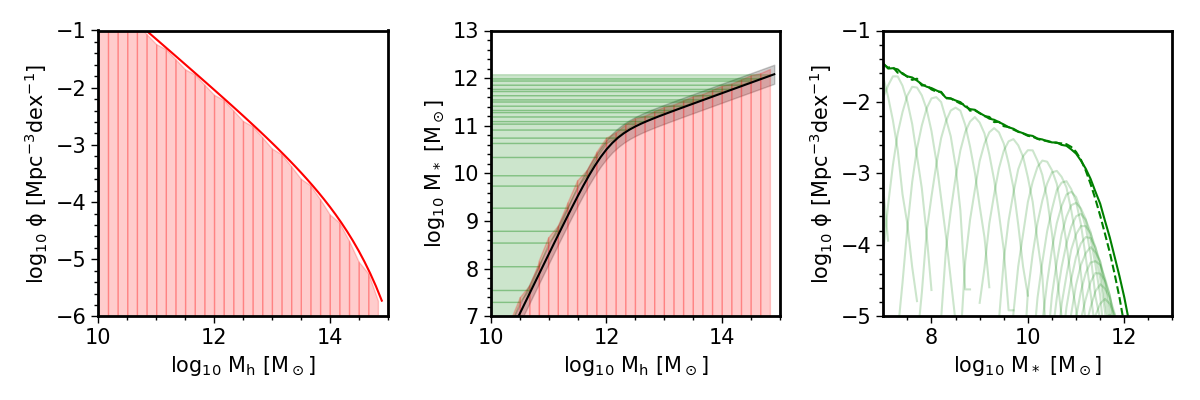
\includegraphics[width = \linewidth]{Figures/Chapter2/gaussian_buildup.png}
    \caption{A cartoon to show how the 'statistical' approach can be taken to transform a HMF to a SMF via number density propagation. From lest to right: Halo mass function with selected binning shown by shaded bands; The SMHM relation with the halo mass bins shown as red bands and the associated stellar mass distributions shown as green bands; The SMF with the Gaussian distributions from each halo mass bin shown as solid green curves that are then summed to create the total stellar mass function. An animated version of this plot made public by PJG can be found at \url{https://twitter.com/RSEGrylls/status/1231279549704474624}.}
    \label{fig:Gauss_build}
\end{figure}

We then fit to the \cite{Davidzon2017TheSnapshots} data both uncorrected and corrected for the cmodel and PyMorph fits respectively (see Section \ref{subsec:SMF} for details). At high redshift we use the central and subhalo mass functions initialising satellites at infall as described above\footnote{Ideally, as for low redshift, we would use the centrals only as we are primarily concerned with the central SMHM relation. However, lacking a well-defined central stellar mass function at high redshift, this method represents a reliable way to extend the model to higher redshifts.}. For central haloes the method is the same as detailed above, however, as we use the total stellar mass functions at high redshift we also include the total unevolved surviving subhalo mass function in the abundance matching. 
We assume that a halo before infall hosts a central galaxy; under this assumption we use the central SMHM relation to assign satellite galaxy stellar mass at the point of accretion. For the latter, we must have information about the redshift of infall for subhaloes. We obtain from \textsc{steel} the unevolved surviving subhalo mass function as contributed by each redshift of infall. Each contributing part is calculated using the SMHM relation at the redshift of infall and added to the central stellar mass function using the same method as with the centrals. The total stellar mass function is compared, at each redshift step available, to the data via the likely-hood function to give the probability that the given point is the `true' evolution parameters. The abundance matching best-fit parameters and associated errors for both the cmodel and PyMorph are given in Table \ref{tab:AbnResult}, and plots showing the cross-sections of the parameter space are shown in Appendix \ref{Appx:AbnMCMC}.

\begin{table}
\centering
\begin{tabular}{l||llll|llll}
        & $M_n$ & $N$     & $\beta$ & $\gamma$ & $M_{n,z}$ & N\_z   & $\beta_z$ & $\gamma_z$ \\ \hline
\\
cmodel  & $11.91_{-0.34}^{+0.40}$ & $0.029_{-0.013}^{+0.018}$ & $2.09_{-1.02}^{+1.21}$    & $0.64_{-0.10}^{+0.11}$     & $0.52_{-0.19}^{+0.24}$       & $-0.018_{-0.004}^{+0.005}$ & $-1.03_{-0.34}^{+0.049}$     & $0.084_{-0.14}^{+0.20}$      \\
\\
PyMorph & $11.92_{-0.36}^{+0.39}$ & $0.032_{-0.012}^{+0.016}$ & $1.64_{-0.73}^{+0.85}$     & $0.53_{-0.11}^{+0.11}$     & $0.58_{0.19}^{+0.15}$        & $-0.014_{-0.006}^{+0.007}$ & $-0.69_{-0.36}^{+0.29}$      & $0.03_{-0.147}^{+0.154}$      
\end{tabular}
\caption{The abundance matching results for the cmodel and PyMorph data. The errors are the 16th and 86th percentile from the MCMC fiting.}
\label{tab:AbnResult}
\end{table}

\begin{figure}[h]
    \centering
    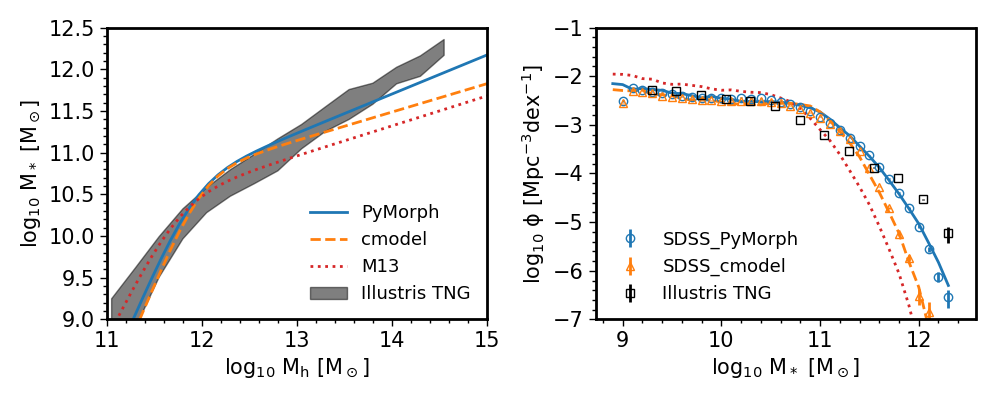
\includegraphics[width = \linewidth]{Figures/Chapter2/AbundaceMtch_Data.png}
    \caption{Left: The SMHM relation at redshift $z=0.1$. The PyMorph (blue solid line) and cmodel (orange dashed line) fits from this work are both for central haloes/galaxies, the fit from \citet{Moster2013} (M13, red dotted line) is for all haloes/galaxies. The grey band is the relation from Illustris TNG100. Right: Stellar mass functions created using the central halo mass function and the three SMHM relations compared to PyMorph (blue circles) and cmodel (orange triangles) central stellar mass functions. The black squares are the stellar mass function from Illustris TNG100.}
    \label{fig:Abn_Data}
\end{figure}

In Figure \ref{fig:Abn_Data} we show the results of our abundance matching to the PyMorph and cmodel central stellar mass functions. The PyMorph fit is steeper above the knee compared to either the cmodel or the \citet{Moster2013} model fits, as expected given the larger number density of massive galaxies found applying the S\'ersic-Exponential model \citep[eg.,][]{Shankar2014, Kravtsov2018StellarHalos}. The low mass slope for both PyMorph and cmodel are almost identical as the galaxies in this range are not affected by the photometric choice. Differences between the fits from this work and \citet{Moster2013} are due to our selection of using only central haloes/galaxies as opposed to the total population, and the stellar mass functions shown in the right-hand panel are lower than even cmodel are therefore missing massive galaxies.


\subsection{Continuity star formation rate}

A substantial modelling problem arises from the continuity between the evolution of the SMF and the observed SFR. The observed UV star formation rates applied to high redshift stellar mass functions when evolving populations conserving number density between epochs yield stellar mass functions higher than those observed. This deviation led to models which can not simultaneously reproduce the observed SFR and SMF, without invoking harsh feedback routines.

\begin{figure}[h]
    \centering
    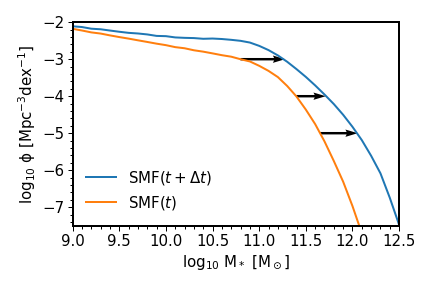
\includegraphics[width = \linewidth]{Figures/Chapter2/ContinuityEqn.png}
    \caption{The continuity approach connects at constant number density galaxy populations across cosmic time. Between two epochs `$t$' and `$t + \Delta t$' the SMF grows differently at different number density. The mass difference, $\Delta M$, indicated at three number densities by black arrows is the expected mass growth for each population.}
    \label{fig:Cont_Eqn}
\end{figure}

The continuity star formation rate is a theoretical quantity calculated such that the observed growth of the stellar mass function is conserved. As illustrated in Figure \ref{fig:Cont_Eqn} by connecting two SMF at consistent number density at times `$t$' and `$t + \Delta t$' the growth in mass $\Delta M$ at each number density over the time $\Delta t$ is obtained. In the simplest approximation, the SFR is equal to $\Delta M / \Delta t$. However, the observed star formation rate is higher than the this value. As new stars are created a proportion of the mass is recycled through supernova `quickly' in terms of cosmological time. This mass recycling given in \citet{Moster2018Emerge10} is used to amend the star formation rate, to account for the mass loss based on the entire star formation history of the galaxy. The fraction of mass lost by a population of stars over time $\tau_{ml}$ is given by,

%Mass recycling
\begin{equation}
\label{eqn:f_ml}
f(\tau_{ml}) = 0.05 \ln \Big(\frac{\tau_{ml}}{1.4 Myr}+1\Big),
\end{equation}

summing the difference in fraction lost in a time step $\delta t$ for every star formation epoch in the galaxies history (SFH) gives the mass loss rate (MLR), 

\begin{equation}
\label{eqn:MLR}
MLR(t) = \frac{ \sum_{t' = t_{inf}}^{t} SFH(t')(f[t' - (t-\delta t)]-f[t' - t]) }{\delta t}.
\end{equation}

The continuity SFR is therefore calculated to be $\Delta M / \Delta t$ + MLR. The final correction made to this star-formation rate is that galaxies also accrete mass via mergers this accrete mass term ($M_{acc}$) is prominent for massive galaxies $M_* > 10^{11} M_{\odot}$. The continuity SFR at time t' is then finally,

\begin{equation}
    SFR_{continuity}(t') = \frac{\Delta M(t')}{\Delta t} + MLR(t') - M_{acc}(t').
\end{equation}

\subsection{Empirical central galaxy growth}

Using the stellar-mass-halo-mass (SMHM) relation and halo mass growth histories (HMGH) we make an empirical prediction of the average central galaxy growth. In Figure \ref{fig:Cent_Mass_PP} we show in the top left the HMGH for two haloes $M_{z=0} = 10^{14}, 10^{12.5} M_{\odot}$, the middle panel shows the SMHM where the shading shows the extent of the evolution of the median of the relation over the redshift range, finally the bottom left shows the stellar mass growth history (SMGH) predicted by the latter two inputs.

%include a plot of using AM to convert HMGH to SMGH?
\begin{figure}[h]
    \centering
    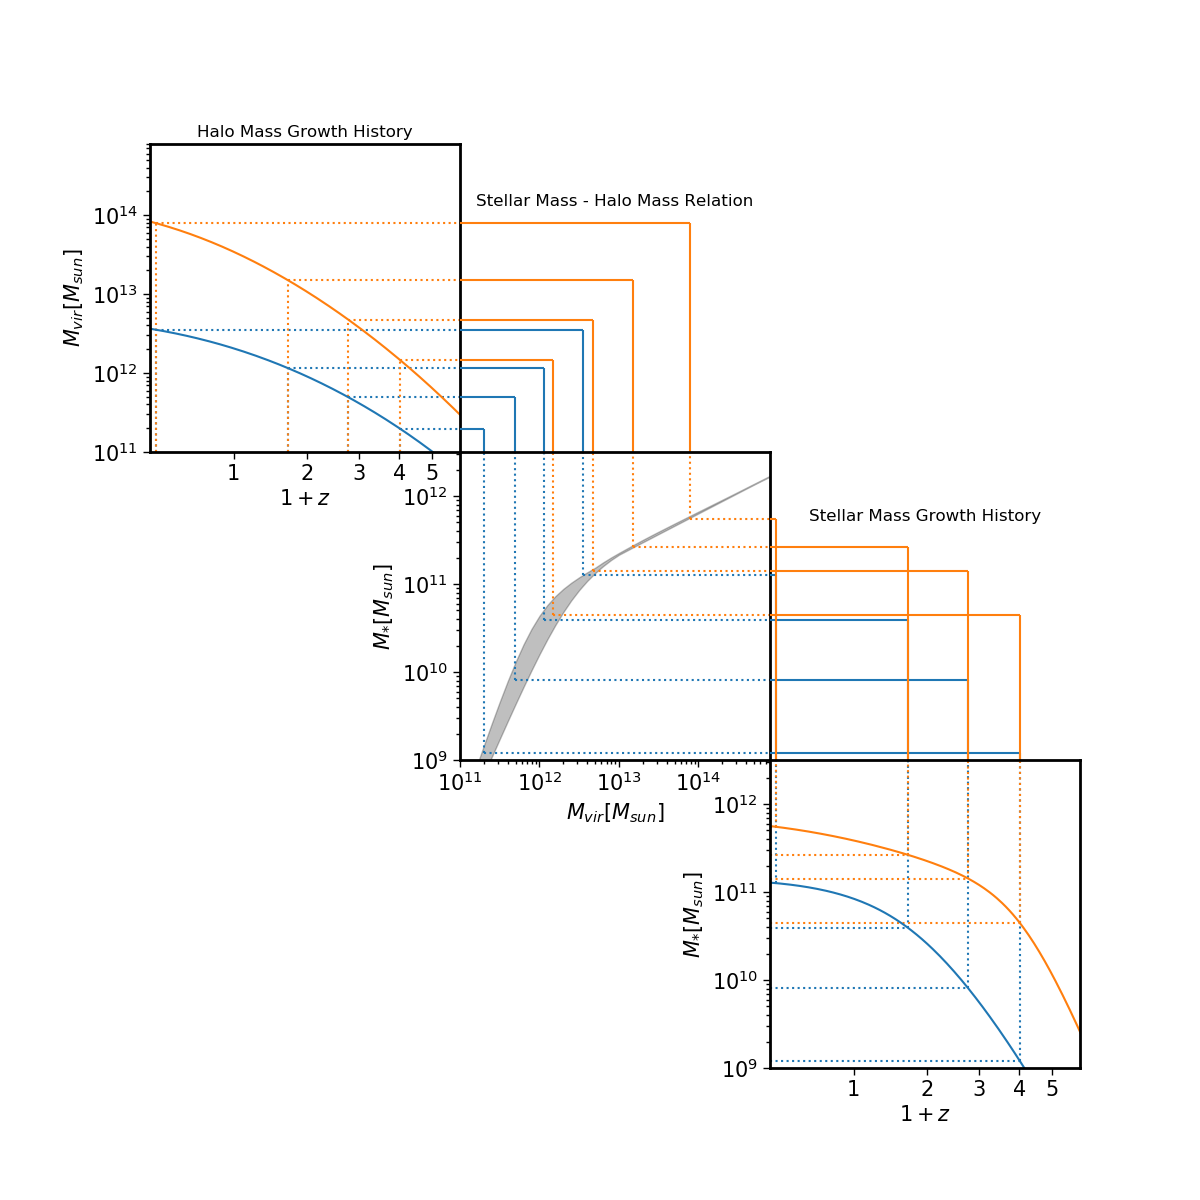
\includegraphics[width = \linewidth]{Figures/Chapter2/HMGH_to_SMGH.png}
    \caption{The Halo Mass Growth Histories (HMGH, top-left) are propagated through the redshift dependent stellar-mass-halo-mass relation (SMHM, middle) to produce corresponding Stellar Mass Growth Histories (SMGH, bottom-right). The lines illustrate matching points in redshift and the intersection with the SMHM relationship. The width of the SMHM relationship shows the extent of evolution with time, not as is common the scatter.}
    \label{fig:Cent_Mass_PP}
\end{figure}

At several redshift epochs, the HMGH to the SMGH are connected following the colour-coded lines, it is found the shape of the SMHM relationship is the primary factor that dictates the shape of the SMGH. Identifying for each growth history the step before the central galaxy growth rapidly slows $z = 3$ for orange and $z = 1$ for blue each of these lines intersect the HMGH when it is still growing, whereas they intersect the SMHM relationship just before the `knee'. This change in the growth behaviour is thought to be an effect of active galactic nuclei suppressing the formation of stars in a galaxy. However, as the knee is a function of halo mass once could also attribute this to the halo mass at which infalling gas is shock heated and can no longer efficiently accrete to the central galaxy.

\section{Discussion}

This chapter has outlined the core methodologies of \steel as they stood at the time of writing. For exact details of the development of the methods we refer the reader to the full papers in Appendix \ref{Appx:Papers}. For example, the continuity star formation rate in \Paper{1} was derived by generating SMF at subsequent time-steps and then following populations at consistent number density; In \Paper{2} the method was updated to instead follow the central dark matter growth histories. 

At it's inception \steel was a short test script we were using to try to test what the maximum number of satellites in a halo given a SMHM relation. The 75 line code in Section \ref{sec:Proof} is a recreation of the original script with additional formatting and commenting\footnote{Note this script will not run as the SMHM relation called from SEM is not present neither are the parameters to be sent to that script. The naming conventions are as originally used being a patchwork of other scripts. trapz is a simple trapezium integrator that would also need to be replaced. This script is unlicensed and only intended as a guide to the original thoughts that went into building the foundation of \steel}.

\section{Future}

As will be seen in the following Science Chapters (3, 4, \& 5) the novelty of \steel provides a view on galaxy formation physics that can refresh and re-frame some ideas in the field. However, as \steel grew naturally from the proof of concept, it has now reached a stage common to many software programs where it requires a critical tear down and refactor. Developing \steel is possible only for PG and those trained by PG without a significant time investment, therefore a refactor will provide the following usability and science benefits. 
\begin{itemize}
    \item Development ease: A redesign of the software architecture will make the addition of new modules easier important for retaining flexibility.
    \item Method: Many of the routines in steel involve weighted statistical distributions (mostly small gaussian scattering) it would therefore be in the interests of the model to redesign the methodology around an object orientated approach that handles many probability distribution convolutions by design.
    \item Speed: \steel is much faster than most models as is the design spec, however, the choice of \textsc{python} as the language has had certain drawbacks.  Iterative process are slow, for this reason the entire starformation module was written in \textsc{cython} a type defined version of python that is pre-compiled into \textsc{c}, this process is both slow and difficult. With a full refactor the choice of language and acceleration tools could be more carefully considered with the end product known.
    \item Science: Many requests have been made of \steel by others recognising it as a potentially revolutionary tool, some are possible but hard, for example adding gas fractions requires a 4th dimension to be added to the running/output data. Others are (near)impossible under the current logic of the code such as creating partitions in the central population and treating each population differently. These again could be designed into a full refactor.
    \item Output: The data output from \steel and the 'post-processing' modules are messy. The simple initial models could save files by name with only 9(/18) parameter combinations that were of interest. This has not scaled well and a full rethink of the data handling, model launching, and output plotting is sorely required.
    \item Integration: Relying on all the above \steel has been proposed by PJG as a necessary analysis tool for ensuring the self consistency of future extra-galactic surveys. Further details will be given in Chapter \ref{Chapter:Conclusion} and a technical outline can be found in Appendix \ref{Appx:HF} where a 4 year fellowship outline of work can be found.
\end{itemize}

\pagebreak
\section{Proof of concept}
\label{sec:Proof}
\inputminted{python}{Codes/Proof.py}
 % Describing STEEL. What, why and how... 

% Chapter 3

\chapter{Understanding the origins of the satellite galaxy distribution in central haloes.} 
\label{Chapter:GalDist}
\lhead{Chapter 3. \emph{Satellite Distributions}} % Write in your own chapter title to set the page header
\begin{center}
    \textit{With more purpose than the course your life was on \newline
    But if you haven't seen the places you have come from\newline
    Then you haven't seen how far you have come\newline
    In the bigger picture, there's a star sixteen times fainter\newline
    In the bigger picture, there's a course seventeen times straighter\newline
    In the bigger picture, there's a dream eighteen times greater\newline
    And it'll steer you like no other, in the bigger picture...\newline}
Stornoway - `The Bigger Picture'
\end{center}


\section{Background}
%What do we know about the distributions of galaxies
In the \LCDM model of the universe growth of haloes is hierarchical.  This results in dark matter substructure and the stellar-mass-halo-mass relation implies that galaxies should be similarly clustered. Satellite galaxies situated in dark matter clusters can therefore be used as tracers of dark matter and used to constrain the cosmological parameters withing a given \LCDM cosmology.
In this chapter we explore the ability of \steel to reproduce satellite distributions over multiple epochs. \steel is also used to test the affect of changing: the dynamical friction timescale, stripping of satellite stellar mass, and star formation rate. By comparing to SDSS data we are able to identify the magnitude of each of these affects on the satellite distribution. Understanding the strength of these effects is crucial to understanding the nature of satellites and their mergers with central galaxies.  

\section{Halo Structure and Dynamical Friction}

To understand the evolution of the subhalo/galaxy population we need to isolate which subhalo mass bins from the unevolved subhalo accretion history survive to following epochs. The sum of all the surviving subhaloes (at each epoch) then yields the unevolved surviving SHMF. 

\subsection{Sub-halo Merging Timescale}
\label{sec:Timescale}
 A key parameter used to calculate the unevolved surviving SHMF is the ``observability timescale'' (or survival time) of each  subhalo mass bin $[M_{h,sat}(z),$ $M_{h,sat}(z) + dM_{h,cent}(z)]$ associated to a parent halo mass bin $[M_{h,cent}(z),$ $M_{h,cent}(z) + dM_{h,cent}(z)]$. This timescale is equivalent to the merger timescale $\tau_{merge}$ of a subhalo of mass $M_{h,sat}$ in a parent halo mass $M_{h,cent}$. To calculate $\tau_{merge}$ we use the routines in Equation \ref{eqn:Tmerge} derived from N-body simulations \citep{Boylan-Kolchin2008},

\begin{equation}
\label{eqn:Tmerge}
\tau_{merge} =
(f_{t_{dyn}}\tau_{dyn}) \frac{A(M_{h, cent}/M_{h,sat})^B}{\ln(1+M_{h, cent}/M_{h, sat})} \exp \Big(C\frac{J}{J_c(E)}\Big) \Big( \frac{r_c(E)}{r_{vir}} \Big)^D,
\end{equation}

where A=0.9, B=1.0, C=0.6, D=0.1 \citep{McCavana2012TheMergers}. The factor $\tau_{dyn}$ is given by \citep{Jiang2016StatisticsFunctions},

\begin{equation}
\label{eqn:tdyn}
%t_{dyn} = N \cdot 0.1 \cdot {H(z)}^{-1} 
\tau_{dyn} = 1.628 h^{-1} \mathrm{Gyr} \Big(\frac{\Delta_{vir}(z)}{178}\Big)^{-\frac{1}{2}} \Big(\frac{H(z)}{H_0}\Big)^{-1} \, .
\end{equation}

Our method of considering average halo mass and accretion histories does not permit tracking single orbits and associated orbital energies. We assume instead an average orbit circularity of 0.5 \citep{Khochfar2006OrbitalHalos}, thus reducing the dependence on the angular momentum and radial components, $\frac{J}{J_c(E)}$ and $\frac{r_c(E)}{r_{vir}}$, to a constant. In other words, this approximation is consistent with the approach of taking the average expected orbits of subhaloes at fixed parent halo mass.
The key parameter of our analysis is the factor $f_{t_{dyn}}$ included in Equation \ref{eqn:Tmerge}.
The fudge factor $f_{t_{dyn}}$ takes into account the systematic uncertainties induced by numerical resolution effects in N-body simulations which are unable to resolve the full merging timescales of subhaloes and/or the satellite galaxies they host \citep{vandenBosch2018DisruptionFiction}. The parameter $f_{t_{dyn}}$ increases or decreases the dynamical times of  ``merging'' satellites enabling an exploration of the effect of dynamical time on the final number density distributions of satellite galaxies at any given epoch.

\subsection{Surviving Subhalo Population}
At each redshift we use the unevolved subhalo accretion history and the observability timescale $\tau_{merge}$ to calculate the total `observable' subhalo population associated with any given parent halo mass bin $[M_{h,cent}(z),$ $M_{h,cent}(z) + dM_{h,cent}(z)]$, i.e. the unevolved surviving SHMF (shown by the dashed lines in Figure \ref{fig:SHMF_clus}). To compute the implied total number densities of unmerged subhaloes with mass $[M_{h,sat}(z),$ $M_{h,sat}(z) + dM_{h,sat}(z)]$ at any redshift of interest we convolve the unevolved surviving SHMF with the HMF,

\begin{equation}
\label{eqn:GSHMF}
N(M_{h, sat}, z) =
\int USSHMF\Bigg(\frac{M_{h, sat}}{M_{h, cent}}\Bigg)HMF(M_{h, cent}, z)dM_{h, cent}.
\end{equation}

Figure \ref{fig:SHMF} shows the total observable subhalo population for different  $f_{t_{dyn}}$ similar to the SHMF in Figure \ref{fig:SHMF_clus}. Furthermore, via appropriate abundance matching algorithms, we can assign corresponding satellite galaxies to the unevolved subhalo accretion history and obtain the distribution of satellites in a given parent halo mass bin $[M_{h,cent}(z),$ $M_{h,cent}(z) + dM_{h,cent}(z)]$ by assuming the satellites follow the same merging timescales as their host subhaloes.

\begin{figure}
	\centering
	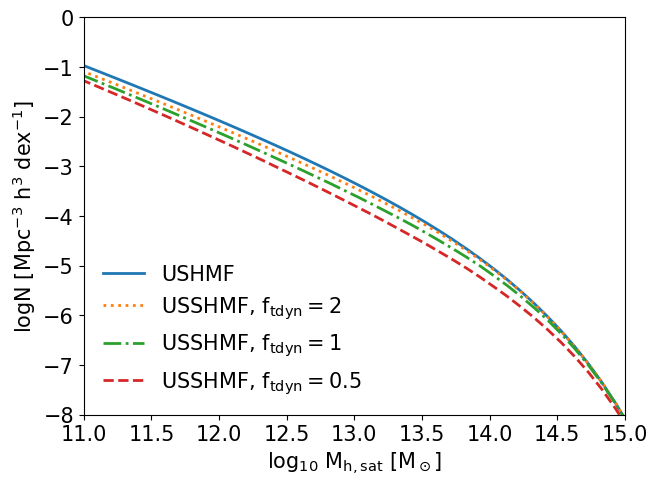
\includegraphics[width = \linewidth]{Figures/Chapter3/SHMF.png}
	\caption{Example of the `total' unevolved SHMF (solid line) and three `total' unevolved surviving SHMF (dotted lines) corresponding to three different $f_{t_{dyn}}$ factors.}
	\label{fig:SHMF}
\end{figure}

\section{Observed Satellite Distributions}

As shown in Equations \ref{eqn:Tmerge} and \ref{eqn:tdyn} the dynamical friction/observibility timescale is dependent on the ratio of halo to sub-halo mass. In Figure \ref{fig:Tdyn_M} in the left hand panel the merging timescales for subhaloes falling into three different central masses at redshift $z=3$ are shown. In each case smaller subhaloes, with lower mass ratios, have longer merging times. Sub-haloes that are significantly under an order of magnitude of the mass of the central halo the merging timescales can extend past $z=0$ and such objects would still be present in halo structures today. Through association of galaxies to subhaloes, via the SMHM relationship at infall, we can repeat the exorcise with satellite galaxies. It is similarly found that small galaxies in massive haloes are the only galaxies accreted at redshift $z = 1.5$ that one would expect to still be observed orbiting local galaxies.

\begin{figure}[h]
	\centering
	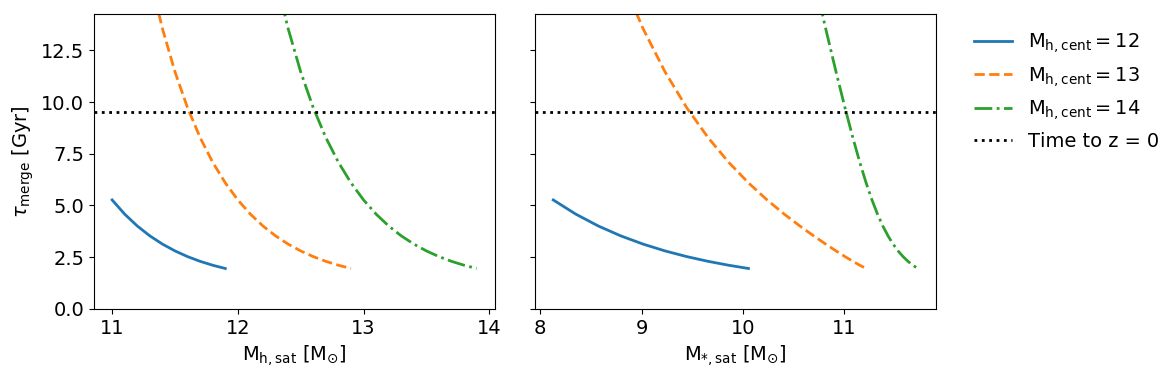
\includegraphics[width = \linewidth]{Figures/Chapter3/Tdyn_M.png}
	\caption{The range of merging timescales for a range of subhalo (left) and satellite (right) masses when accreted at $z = 1.5$ onto three different host masses: $\log$ $M_{h, cen}$ $[M_{\odot}]$ = 12 (blue solid), 13 (orange dashed) and 14 (green dot-dashed). The dotted black line shows the time to redshift $z = 0$, i.e. the minimum amount of time a satellite would need to survive to be observable in the local universe.}
	\label{fig:Tdyn_M}
\end{figure}

In Figure \ref{fig:AccretionTime} the practical affect of increasing the dynamical time is shown. Increasing the dynamical time factor $f_{tdyn}$ to infinity satellites will never merge with the central and thus the right hand panel shows the total buildup of satellites over cosmic time. In the right hand panel with $f_{tdyn} = 1$ we see how the population of satellites still observable at $z=0.1$ is built up over time. As expected from Figure \ref{fig:Tdyn_M} only recently accreted massive satellite galaxies contribute to the observable population where as smaller galaxies will have a wider distribution of accretion times. Notably there are no galaxies, within our mass ranges, accreted before redshift $z=2$ that remain observable at redshift $z=0.1$.

\begin{figure}[h]
	\centering
	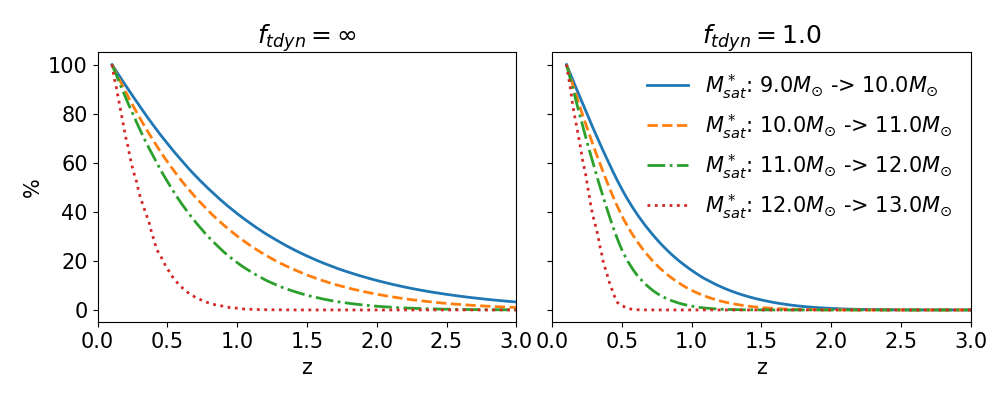
\includegraphics[width = \linewidth]{Figures/Chapter3/AccretedSatellitePercentage.png}
	\caption{We show the percentage of satellites observed at a $z = 0.1$ as a function of their redshift of accretion $z > 0$. It can be seen that massive satellites observed at $z = 0.1$ are accreted more recently than smaller satellites. At $z = 0.5$ less that 50\% of the total satellites observed at $z = 0.1$ have been accreted, and at $z = 0.1$ this falls to less than 20\%. }
	\label{fig:AccretionTime}
\end{figure}

\subsection{Affect of Dynamical Friction}
%Show the dynamical friction model and how that actually impacts the distribution.
In this Section we show the prediction of \steel with different merging timescales, $f_{tdyn}$ = $0.5, 1.0, 2.5$, to probe the effects of dynamical time on the satellite population. In Figure \ref{fig:SMF_Tdyn} we find, as expected, that longer dynamical times tend to increase satellite number densities especially towards lower stellar masses. The number densities of higher-mass satellites are more resilient to increase with dynamical time. In fact, when $f_{tdyn}\gtrsim 1$ the number densities of massive satellites become already very close to the theoretical maximum number density when  $f_{t_{dyn}} = \infty$. This trend is also seen in Figure \ref{fig:AccretionTime} the difference between the buildup of high mass satellites between $f_{t_{dyn}} = \infty$ and $f_{t_{dyn}} = 1$ is much less significant than between that of low mass satellites
It follows that massive satellites are on average a recently accreted population. In other words, there are only a few high mass satellites that had enough time to merge when $f_{tdyn}\gtrsim 1$. In contrast, lower mass satellites have not yet reached their theoretical limit, and thus they still have room to increase their number densities with increasing dynamical time.  

When computing the distribution of satellites as a function of parent halo mass we show both full number densities, as well as fractional distributions to better highlight the ``skewness'' of the predicted distributions with respect to the data. The latter will be simply computed as
\begin{equation}
\label{eqn:FracPlot}
F(dM_h) = \frac{N(>10^x)|_{dM_h}}{N(x)},
\end{equation} 
where $N(>10^{x})$ is the total number (density) of satellites above a threshold stellar mass $x= \log M_{*}$, and the $N(>10^{x})|_{dM_h}$ is the number of these that reside within the halo mass bin $[M_h, M_h+dM_h]$.

Figure \ref{fig:Sat_Dist_Tdyn} shows how as a function of parent halo mass the distribution of satellites, above three stellar mass cuts, is affected by $f_{tdyn}$. The number density distribution (top row) shows results similar to the satellite SMF where increasing dynamical time increases the number densities. However, there is also an apparent steepening effect for which lower mass host haloes end up containing relatively less satellites with respect to models with longer dynamical times. The fractional plot (bottom row) accentuates this change in the number density distributions shown in the top row: shorter dynamical times shift the peak of the distribution to the right as relatively more satellites are observed in high mass host haloes.

This steepening of the satellite distribution as a function of halo mass, as well as the shift of the peak in the lower row, where infinite dynamical times move satellites preferentially to lower halo masses, are both caused by the amount of time satellites survive in their hosts. Massive satellites are far more common in massive hosts, as can be inferred from the SHMF. Therefore, irrespective of the chosen merging timescale, there will always be a high number density of surviving massive satellites in higher mass parent haloes. However, when merging timescales are increased, the lower number densities of massive satellites in moderately-sized haloes are also increased. Given that lower mass parent haloes are more abundant, the reduction of merging timescales tends to shift the peak of the fractional distribution of galaxies to lower mass parents. Otherwise put, the merging timescales in clusters ($ \log_{10} M_{h,cent}$ $[M_{\odot}]$ $> 13.75$) are so long that even a factor five reduction in merger timescale still does not give the satellite galaxies sufficient time to merge with the central galaxy. This effect can be inferred from Figure \ref{fig:Tdyn_M}, where we see steeper gradients for a given subhalo/satellite mass with increasing parent halo mass. Merging is more efficient for the lower mass satellites as can be seen by the steepness of the $f_{t_{dyn}} = 0.5$ model (dashed lines) in the top row of Figure \ref{fig:Sat_Dist_Tdyn}.

%dynamical distributions

\begin{figure}[h]
	\centering
	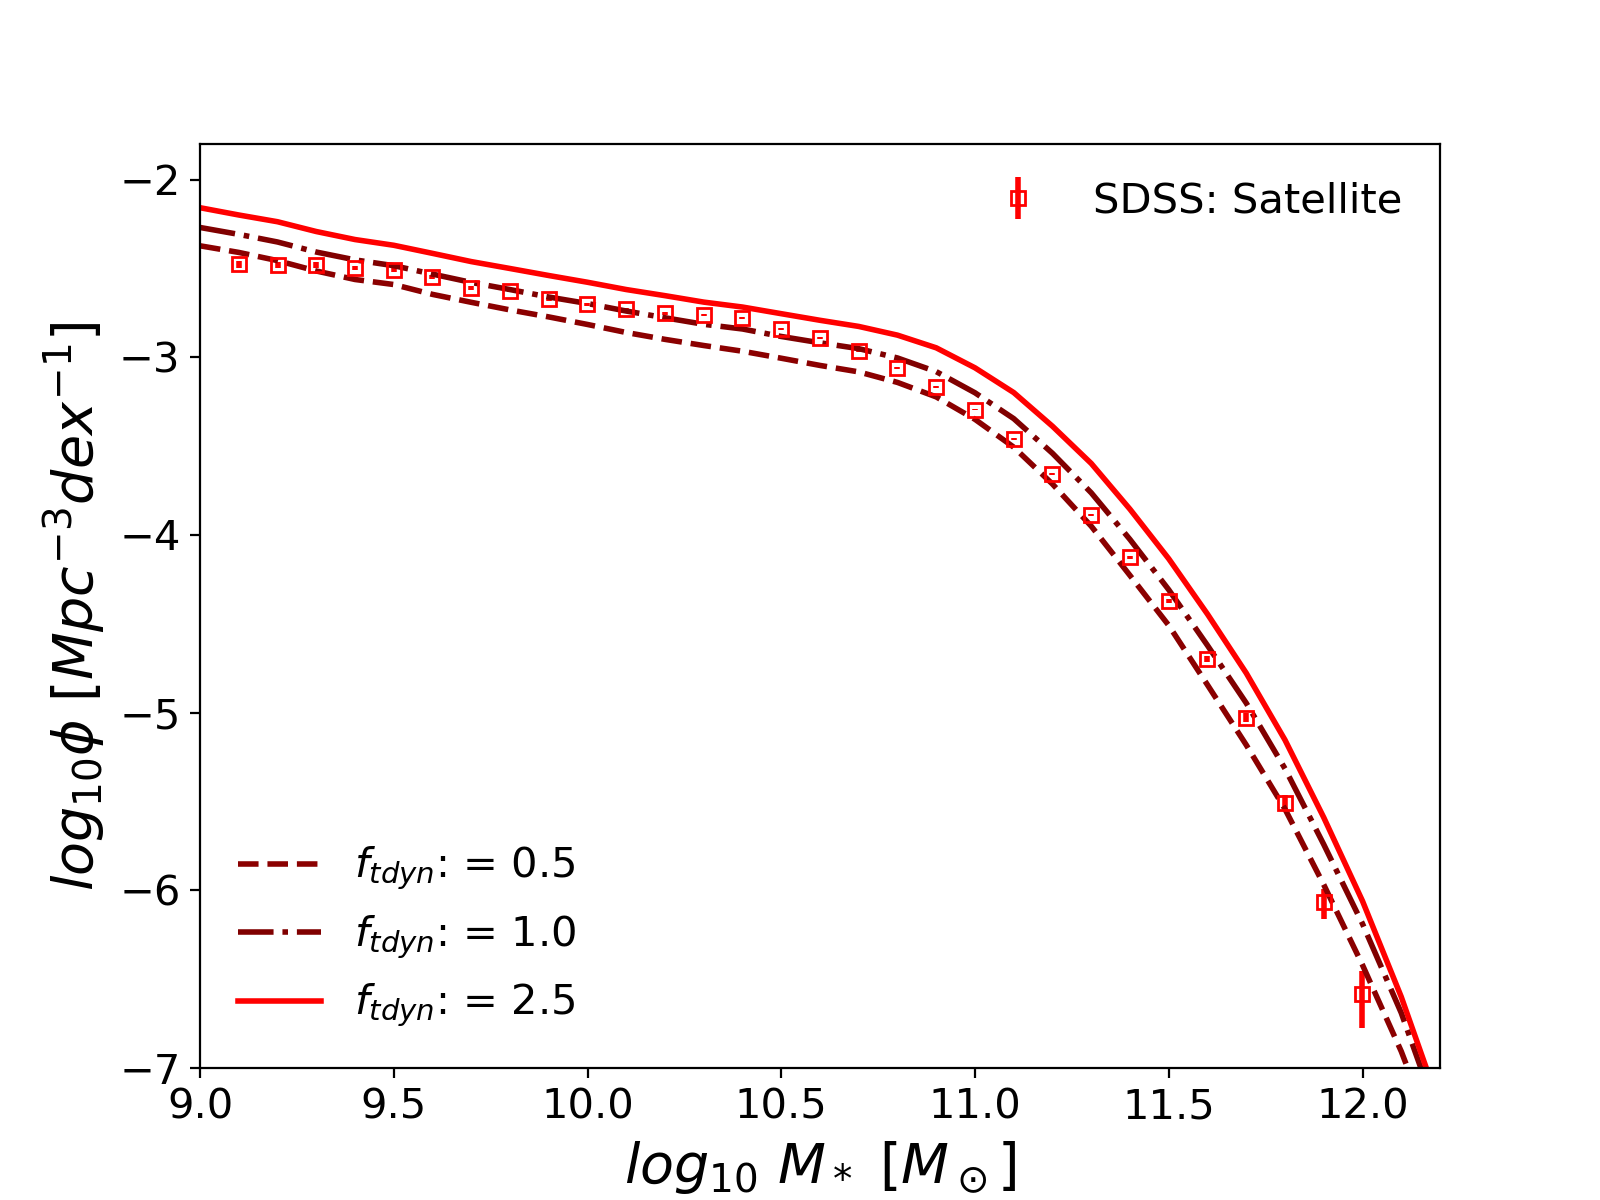
\includegraphics[width = \linewidth]{Figures/Chapter3/Tdyn_SMF.png}
	\caption{Satellite stellar mass functions generated by the model compared to SDSS data (open squares). The solid, dot dashed, and dashed lines show $f_{tdyn} = 0.5, 1.0,$ and $2.5$ respectively.}
	\label{fig:SMF_Tdyn}
\end{figure}

\begin{figure}[h]
	\centering
	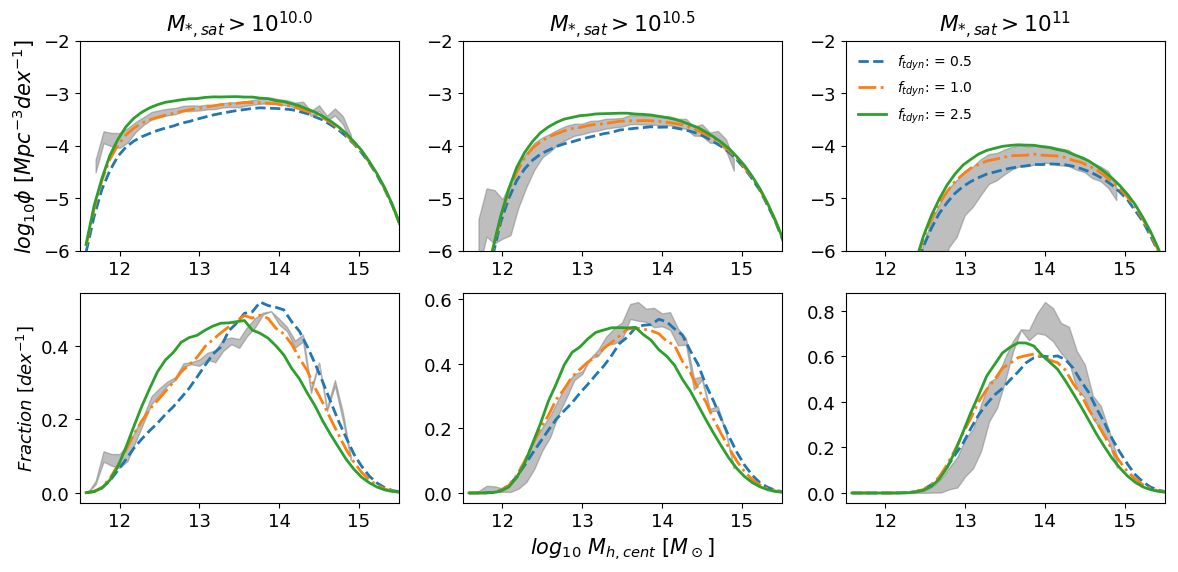
\includegraphics[width = \linewidth]{Figures/Chapter3/Tdyn_Sat_Dist.png}
	\caption{Satellite distributions in parent haloes generated from \steel are compared to those observed in SDSS (grey band). Columns from left to right show increasing satellite stellar mass cuts as labelled. The top row shows the number density of satellites expected to be found in each parent halo mass. The bottom row shows the fractional distribution described by Equation \ref{eqn:FracPlot}. The dashed, dot dashed, and solid lines show $f_{tdyn} = 0.5, 1.0,$ and $2.5$ respectively. The width of the grey band corresponds to a 10\% uncertainty in satellite stellar masses.}
	\label{fig:Sat_Dist_Tdyn}
\end{figure}

The least-square residuals to the SMF, number density distribution and fractional distributions are given in Table \ref{tab:bestfit}. There is no model that simultaneously fully matches all the observations in all mass ranges. The trend in both the number density distribution and the fractional distribution is that slightly longer dynamical times ($f_{tdyn}  = 1.2$) are favoured by the less massive satellites. Longer dynamical timescales better match the halo mass distributions (number density distribution/fractional distributions) for lower mass satellites, and vice versa for higher mass satellites with $\log M_{*}/M_{\odot} >11$. Nevertheless, the simple combination of abundance matching and dynamical merging timescales as suggested by pure N-body simulations ($f_{t_{dyn}} = 1.0$) tends to provide overall good agreement to both the satellite SMF and the satellite distributions, without the need to invoke additional physics in the (late) evolution of satellite galaxies after infall.

\begin{table*}
\centering
\caption{We show the sum of the squared residuals between the SDSS and our model. The satellite SMF is calculated between 9.1 and 12.0 $M_{*}$. The SDF fit is calculated between 12 and 14.9 $M_h$ for the \textgreater10 and\textgreater10.5 plots, and between 12.5 and 14.9 $M_h$ for \textgreater11. The Fractional plot fit is calculated between 11.6 and 14.9 $M_h$.}
\label{tab:bestfit}
\begin{tabular}{c|c|ccc|ccc}
$f_{t_{dyn}}$   & SSMF   (Fig \ref{fig:SMF_Tdyn})               & \multicolumn{3}{c}{SDF  } \vline & \multicolumn{3}{c}{Fractional Distribution } \\
   &   (Fig \ref{fig:SMF_Tdyn})               & \multicolumn{3}{c}{ (Top Row Fig \ref{fig:Sat_Dist_Tdyn}) } \vline & \multicolumn{3}{c}{ (Bottom Row Fig \ref{fig:Sat_Dist_Tdyn})} \\ \hline
            \multicolumn{1}{l}{} \vline & \multicolumn{1}{l}{} \vline & \multicolumn{1}{l}{\textgreater{}10} & \multicolumn{1}{l}{\textgreater{}10.5} & \multicolumn{1}{l}{\textgreater{}11} \vline & \multicolumn{1}{l}{\textgreater{}10} & \multicolumn{1}{l}{\textgreater{}10.5} & \multicolumn{1}{l}{\textgreater{}11} \\ \hline
0.5    & 0.022   & 0.19  & 0.55    & 0.073    & 0.0042 & 0.0047 & 0.0078  \\
0.8    & 0.025   & 0.13  & 0.51    & 0.089    & 0.0020 & 0.0017 & 0.0054  \\
1.0    & 0.034   & 0.12  & 0.56    & 0.10     & 0.0015 & 0.0011 & 0.0050  \\
1.2    & 0.043   & 0.12  & 0.53    & 0.11     & 0.0015 & 0.00094& 0.0046  \\
1.5    & 0.054   & 0.12  & 0.52    & 0.13     & 0.0017 & 0.0010 & 0.0045                              
\end{tabular}
\end{table*}

%show stripping/SF routines and their effects
\subsection{Evolutionary models}

The prior section makes an implicit assumption that satellites do not evolve after infall. In this section we apply several evolutionary affects to the satellites assuming they have the same properties as centrals at infall then evolve both due to in-situ processes and in response to their environment.


\subsubsection{Star Formation Rates}
We use the star formation rate (SFR) parameterization from \citet{Lee2015A1.3} with parameters\footnote{These parameters are derived by fitting data from ZFORGE in combination with far-IR imaging from \textit{Spitzer} and \textit{Herschel} in the range $0.5<z<4$. In this work we extrapolate their fits down to $z = 0$, as this is consistent with the SFR measured by  \cite{Salim2007UVUniverse} at lower redshifts.} from \citet{Tomczak2016THE4} where $s_0$ and $M_0$ have units $log(M_{\odot})$ and $M_{\odot}$ respectively,

\begin{equation}
\begin{split}
\label{eqn:SFR}
\log[\psi(z, M_*)] &= s_0(z) - \log \Big[ 1 + \Big(\frac{M_*}{M_0(z)}\Big)^{-\alpha(z)}\Big] \\
s_0(z) &= 0.195 + 1.157z - 0.143(z^2) \\
\log[M_0(z)] &= 9.244 + 0.753z - 0.090(z^2) \\
\alpha(z) &= 1.118.
\end{split}
\end{equation}

As discussed continuity-equation approaches are more suited to modelling as they avoid the inconsistencies in growth of the SMF and the observed SFR. The novelty in our continuity model with respect to previous work is that we do not tune the resulting star formation rate on the total but rather only on the stellar mass function of \textit{central} galaxies \footnote{ which is in turn iteratively constrained by matching the local stellar mass function of SDSS centrals.}. We use as input for our continuity equation the central SMF generated by the SMHM relation and the central HMF from \cite{Tinker2010THETESTS}. When considering the mass growth we must consider the mass loss, else the SFR is massively under-predicted. We use a instantaneous loss fraction of $40\%$. We also neglect the mass gained from mergers. However, as mergers would decrease the SFR calculated thus this method should be considered an upper limit to the SFR. The fit to the resulting SFRs is given by

\begin{equation}
\begin{split}
\label{eqn:SFR_CE}
\log(\psi(z, M_*)) &= s_0(z) - \log \Big[ 1 + \Big(\frac{M_*}{M_0(z)}\Big)^{-\alpha(z)}\Big] \\
s_0(z) &= 0.6 + 1.22z - 0.2(z^2) \\
\log(M_0(z)) &= 10.3 + 0.753z - 0.15(z^2) \\
\alpha(z) &= 1.3 - 0.1z.
\end{split}
\end{equation}

In all cases the SFR is included in our models with a log-normal scatter of 0.3 dex \citep{Leja2015ReconcilingFunction}.


We also include the ability to quench star formation in satellite galaxies after infall. It has been suggested that satellites undergo a ``delayed-then-rapid'' quenching \citep{Wetzel2013GalaxyUniverse}. The latter model envisions that satellites continue to form stars at the same rate as central galaxies of comparable stellar mass for a time $\tau_q$ after infall, and then quench rapidly over a timescale $\tau_{f}$. This quenching is proposed for satellites with stellar mass above $M_*\gtrsim 10^9 M_{\odot}$, with a minimum $\tau_q$ $\sim$ $1$ $Gyr$. For galaxies below $M_* \lesssim 10^{9} M_{\odot}$, we however adopt the more recent results by \citet{Fillingham2016UnderStripping}, who put forward a parent halo mass dependent cutoff,
\begin{equation}
\label{eqn:Cutoff}
log(M_{cutoff}) = 9 log(M_{\odot}) - (15 log(M_{\odot}) - log(M_{h,host}))/5log(M_{\odot}) ,
\end{equation}
below which satellite galaxies all share the same quenching time $\tau_q=2 Gyr$.
The rapid quenching timescale $\tau_{f}$ can be expressed as \citep{Wetzel2013GalaxyUniverse},
\begin{equation}
\label{eqn:tauf}
\tau_f = -0.5 log(M_{*,sat}) + 5.7Gyr .
\end{equation}
We set a minimum $\tau_{f}$ of $0.2$ $Gyr$ for all galaxies. This rapid quenching begins at times $t > \tau_q$ after infall, and it is approximated by an exponential decay which is longer for larger satellites, as can be inferred from Equation \ref{eqn:SFR_Quench}. The look-back time at which a galaxy begins fast quenching is then $t_q = t_{infall} - \tau_q$. After this time the satellite no longer follows the SFR of a typical central galaxy. Figure \ref{fig:QuenchFig} illustrates the quenching model where the dashed/coloured lines demonstrate the halo mass dependence in cutoff mass.

\begin{figure}
	\centering
	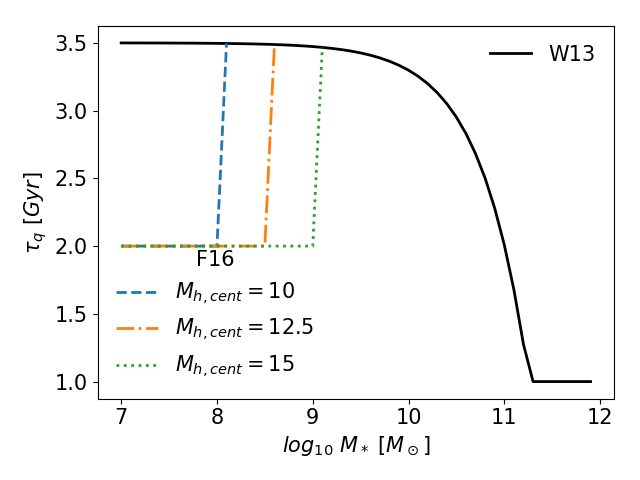
\includegraphics[width = \linewidth]{Figures/Chapter3/Fig4.png}
	\caption{The solid line shows the \citet[][W13]{Wetzel2013GalaxyUniverse} model for quenching. The dashed lines show the host halo dependent reduction in quenching time from \citet[][F16]{Fillingham2016UnderStripping} for three example host masses $\log10$ $M_{h, cent} = 10, 12.5, 15$ as labelled. Larger hosts are able to reduce the quenching time of larger satellites}.
	\label{fig:QuenchFig}
\end{figure}

The SFR during the satellite infall is then given by

\begin{equation}
\label{eqn:SFR_Quench}
SFR(t, M_*) = SFR(t, M_*)
\begin{dcases}
\psi(z(t), M_*), & \text{} t > t_q \\
\psi(z(t_q), M_*)e^{\big[-\frac{t_q-t}{\tau_f}\big]}. & \text{} t < t_q
\end{dcases}
\end{equation}

If at any point a satellite galaxy has a SSFR below $10^{-12}$ $M_{\odot}$ $yr^{-1}$, it is assumed to be fully quenched and assigned a SSFR of $10^{-12}$ $M_{\odot}$ $yr^{-1}$, plus a log-normal scatter of 0.3 dex.


The first, purely observationally-based, star formation rate model strictly follows the SFR parametrization by \citet[][T16 hereafter]{Tomczak2016THE4}, given in Equation \ref{eqn:SFR}. The second star formation rate model (which we label as ``CE'') is instead based on the continuity equation approach. 

\begin{figure}
	\centering
	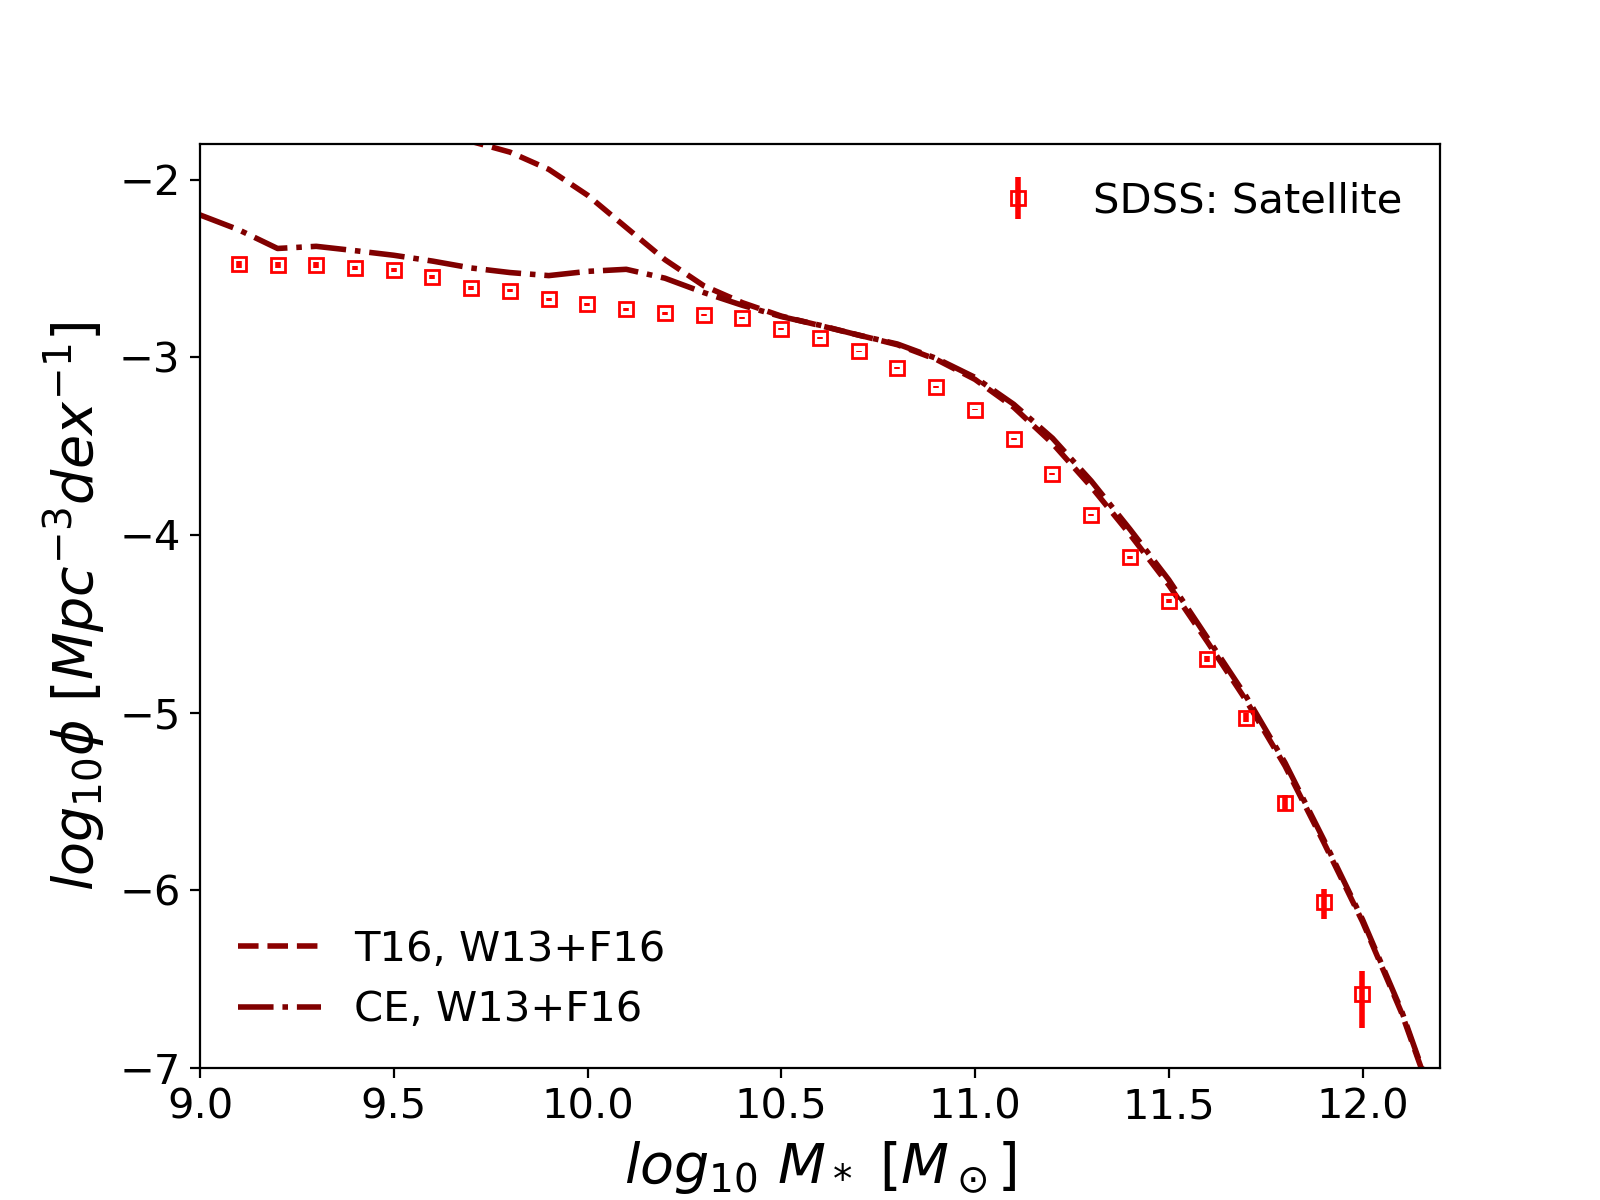
\includegraphics[width = \linewidth]{Figures/Chapter3/Fig9.png}
	\caption{Satellite stellar mass functions generated from the model using both the \citet{Tomczak2016THE4} (dashed) and continuity (dot dashed) star formation rates compared to the SDSS satellite stellar mass function (open squares).}
	\label{fig:SMF_SF_Q}
\end{figure}

We compare the satellite SMFs produced by the two star formation+quenching models addressed above to our SDSS stellar mass function of satellites in Figure \ref{fig:SMF_SF_Q}. It is apparent that using the observed SFR by T16 (dashed line), even inclusive of the best recipes for quenching, still substantially overproduces the number density of galaxies below $M_* \lesssim 3\times 10^{10}\, M_{\odot}$. This is a well-known problem affecting the full (dominated by central) galaxy population \citep[e.g.,][]{Leja2015ReconcilingFunction}: the integrated (observed) SFR is not consistent with the moderate growth over time of the SMF causing an overproduction of galaxies becoming gradually more severe at lower stellar masses. Our results show a similar problem affecting the satellite population, on the assumption that the latter at infall share the same SFR distribution as a typical central galaxy of the same stellar mass.


We now show the relative impact of star formation rate and stellar stripping on the satellite stellar mass function. Figure \ref{fig:SMF_SF_Strip} and Figure \ref{fig:Sat_Dist_SF_Strip} show stellar mass function and host halo mass distributions for the $f_{tdyn} = 1.0$ reference model with no stripping nor star-formation, the CE star formation model, and the CE star formation model with stripping (long-dashed, dot-dashed, and solid lines, respectively). We see from both Figures that the reference and star-formation model are almost indistinguishable. The stripping, at least at the level implemented in this work, also has a rather minor effect, at the most reducing the number densities of the most massive satellites ($>10^{11}M_{\odot}$) by $\lesssim 0.2$dex.

\begin{figure}
	\centering
	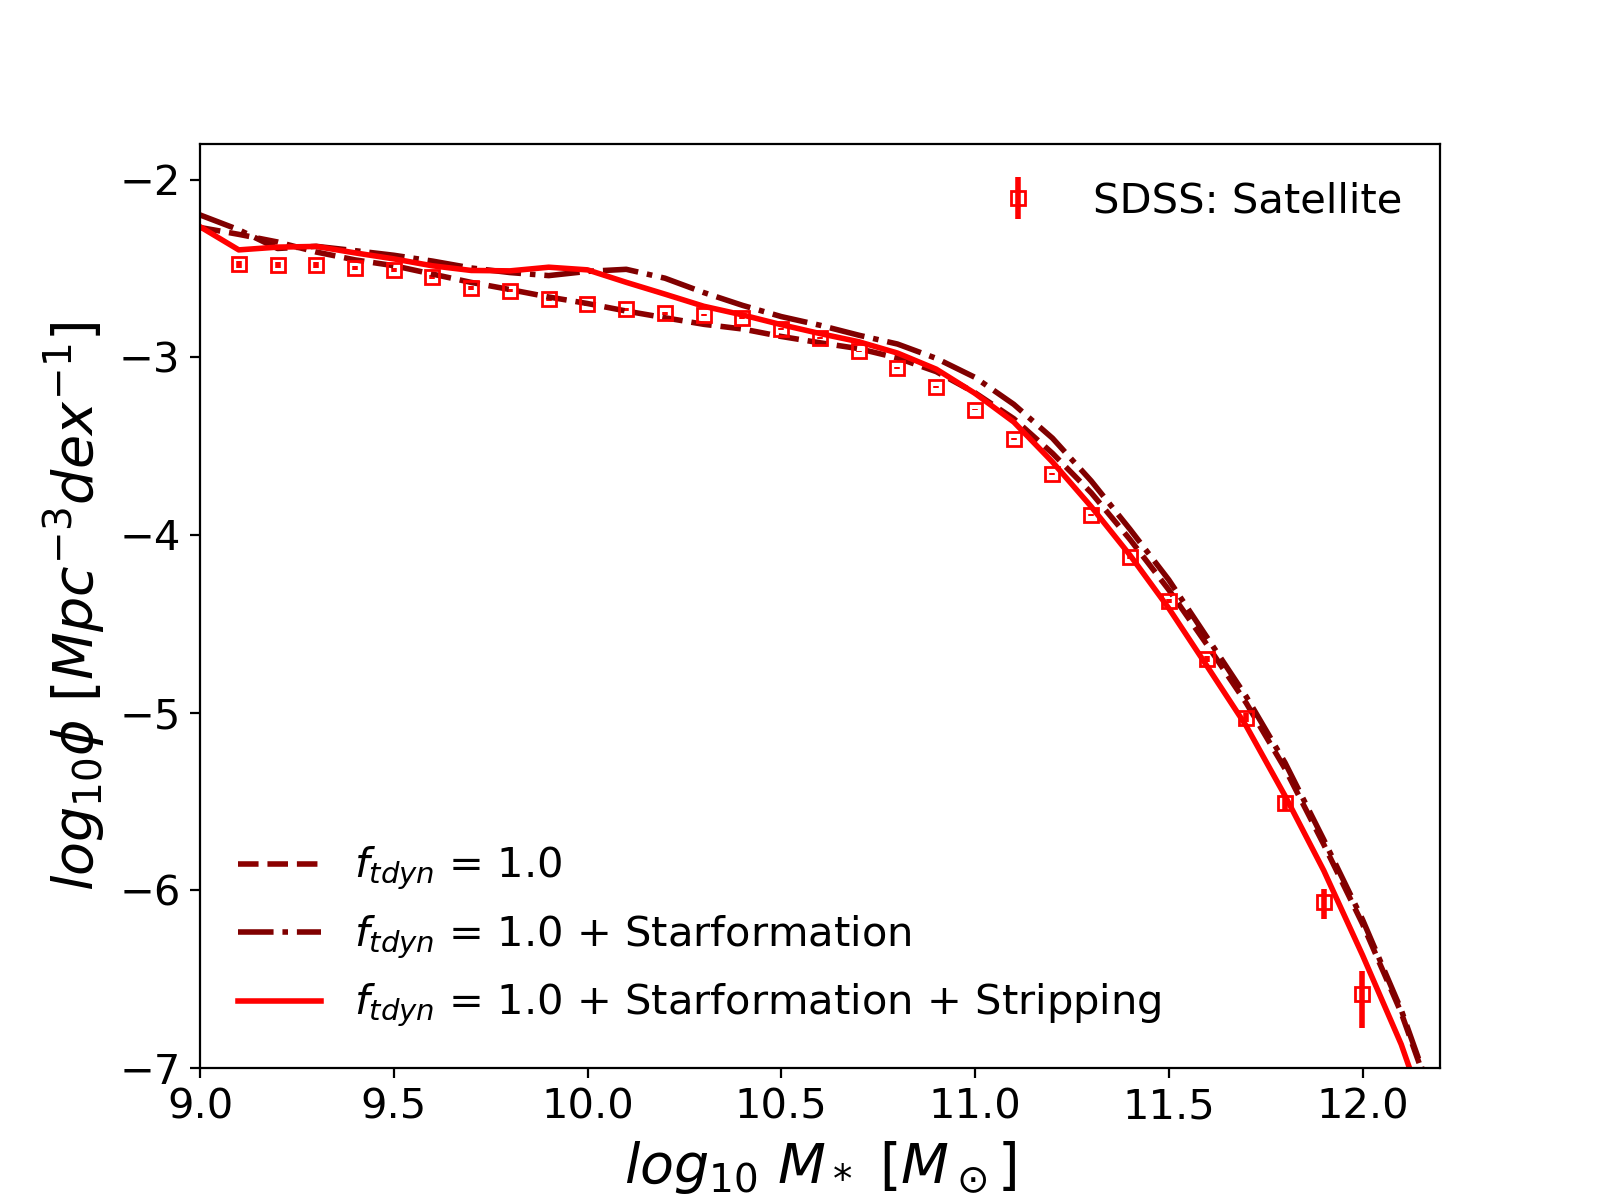
\includegraphics[width = \linewidth]{Figures/Chapter3/Fig11.png}
	\caption{Satellite stellar mass functions generated from the model compared to SDSS satellites (open squares). The models shown all have $f_{tdyn} = 1.0$ and are the reference `frozen model' (dashed line), starformation (CE model) only (dot dashed line) and starformation and stripping (solid line).}
	\label{fig:SMF_SF_Strip}
\end{figure}

\begin{figure}
	\centering
	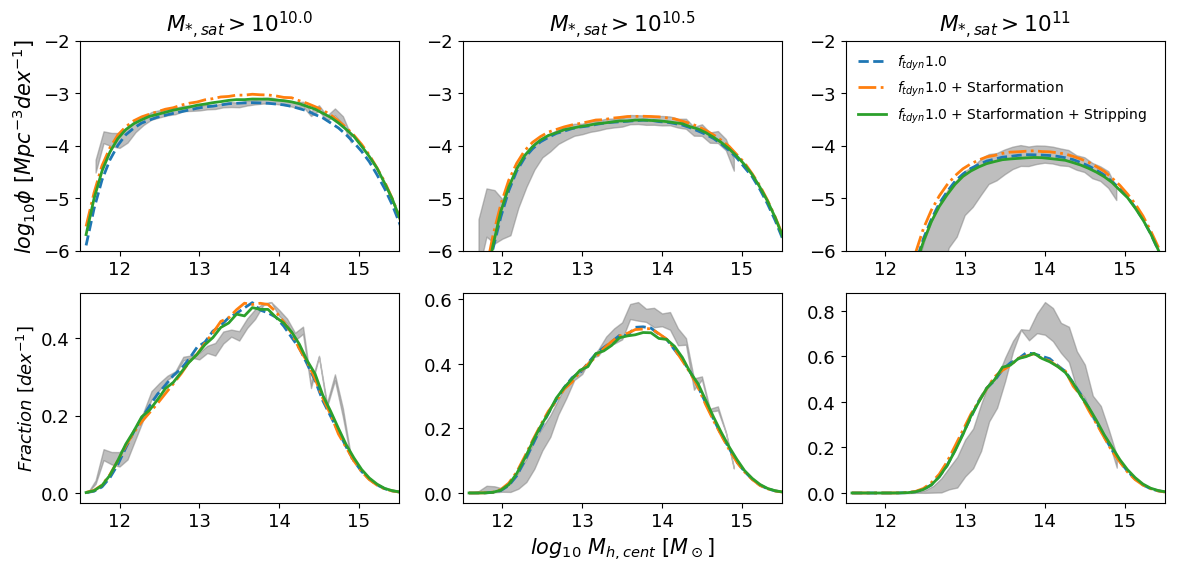
\includegraphics[width = \linewidth]{Figures/Chapter3/Sat_Dist_SF_Strip.png}
	\caption{Satellite distributions in parent haloes generated from the model are compared to those observed in SDSS (grey band). Columns from left to right show increasing satellite stellar mass cuts as labelled. The top row shows the number density of satellites expected to be found in each parent halo mass. The bottom row shows the fractional distribution described by Equation \ref{eqn:FracPlot}. The models shown all have $f_{tdyn} = 1.0$ and are the reference 'frozen model' (dashed line), starformation only (dot dashed line) and starformation and stripping (solid line). The width of the grey band corresponds to a 10\% uncertainty in satellite stellar masses.}
	\label{fig:Sat_Dist_SF_Strip}
\end{figure}

\begin{table*}
\centering
\caption{We show the sum of the squared residuals between the SDSS and our model as in \ref{tab:bestfit} with the same mass ranges for the fitting. All models have $f_{t_{dyn}} = 1.0$ from top to bottom we then have the reference frozen model, the model with starformation, and the model with stripping and starformation.}
\label{tab:SF_Strip}
\begin{tabular}{c|c|ccc|ccc}
$f_{t_{dyn}}$   & SSMF   & \multicolumn{3}{c}{SDF  } \vline & \multicolumn{3}{c}{Fractional Distribution } \\
   &   (Fig \ref{fig:SMF_SF_Strip})               & \multicolumn{3}{c}{ (Top Row Fig \ref{fig:Sat_Dist_SF_Strip}) } \vline & \multicolumn{3}{c}{ (Bottom Row Fig \ref{fig:Sat_Dist_SF_Strip})} \\ \hline
            \multicolumn{1}{l}{} \vline & \multicolumn{1}{l}{} \vline & \multicolumn{1}{l}{\textgreater{}10} & \multicolumn{1}{l}{\textgreater{}10.5} & \multicolumn{1}{l}{\textgreater{}11} \vline & \multicolumn{1}{l}{\textgreater{}10} & \multicolumn{1}{l}{\textgreater{}10.5} & \multicolumn{1}{l}{\textgreater{}11} \\ \hline
1.0 & 
0.034 & 0.12 & 0.53 & 0.10 & 0.0015& 0.0011& 0.0049\\
\begin{tabular}[c]{@{}c@{}}1.0\\ With Star Formation\end{tabular} & 
0.049 & 0.077& 0.43 & 0.14 & 0.0018& 0.0012& 0.0059\\
\begin{tabular}[c]{@{}c@{}}1.0\\ With Stripping and Star Formation\end{tabular} & 
0.021 & 0.087& 0.47 & 0.088& 0.0016& 0.0015& 0.0056
\end{tabular}
\end{table*} 

Table \ref{tab:SF_Strip} shows the sum of the square residuals to the SMF, SDF and fractional distributions for the same models discussed above, our reference frozen one, and the one with evolution of satellites after infall (stellar stripping and continuity equation-based star formation). Table \ref{tab:SF_Strip} shows that the satellite late evolution has little effect on the fractional distribution. In the number density distribution we see an improved fit for galaxies in the $M_*>10.^{11}\, M_{\odot}$ range, mainly induced by the stripping which slightly reduces the number density of massive galaxies. Table \ref{tab:SF_Strip} shows the sum of square residuals for the dynamical time with $f_{t_{dyn}}=1$, for the frozen and evolved models. 

\section{Multi-Epoch Distributions of Satellite Galaxies}

We here extend the group and cluster satellite richness analysis to high redshift. Above it is found that dynamical friction and, to a second order, abundance matching, are the dominant factors in the distribution of satellite galaxies in groups and clusters above $M_{*,sat} > 10^{10} M_{\odot}$. Here, for a more rounded view of the satellite galaxy population, we display the results for the full \textsc{steel} model which includes star formation, dynamical quenching and stripping to evolve satellites after infall. The latter effects, despite being of lower order than dynamical friction or abundance matching, are included to be able to compare to data other than cluster richness, such as the satellite specific star formation rate distribution.

\begin{figure}[h]
	\centering
	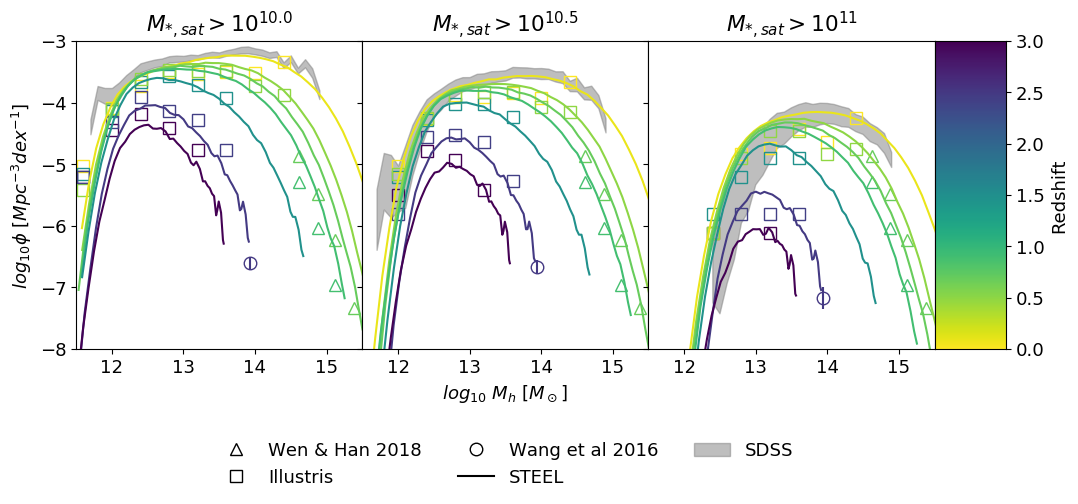
\includegraphics[width = \linewidth]{Figures/Chapter3/HighzClusters.png}
    \caption{The number-density distribution of satellites per parent halo mass predicted from \textsc{steel}, using the PyMorph SMHM relation, at multiple redshift epochs (solid lines). The grey band is the data from SDSS at redshift $z=0.1$. Also included are the high redshift cluster data from \citet{Wang2016DISCOVERY2.506} (circles) and \citet{Wen2018ARedshifts} (triangles). I also compare to the outputs from the Illustris simulation using the TNG100 data (crosses). Each data point and line are given a colour associated to their redshift (the bar on the right provides the color coding key).}
	\label{fig:Sat_Dist_High_z}
\end{figure}

Figure \ref{fig:Sat_Dist_High_z} shows the satellite number density per halo mass bin. For each central halo mass the cosmic number density, similarly to the number density presented in the cumulative stellar mass functions, is calculated for satellites above a mass threshold for each halo mass bin.
The predicted halo richness from \textsc{steel}, using the PyMorph SMHM relation, is shown in this plot as solid lines. The predictions from the Illustris TNG100 simulation \citep{Nelson2018FirstBimodality, Springel2018FirstClustering} are shown with crosses.  Low redshift SDSS data are shown as a grey band, cluster data detailed in Section \ref{subsec:Clusters} are open symbols. The markers and lines in the figure are colour coded based on redshift, as indicated by the colour bar on the right.

\section{Discussion}

There is vast literature on the modelling of satellite galaxies. Here we recall examples of semi-empirical and semi-analytic models to highlight some of the key similarities and key differences. \citet{Neistein2013A2011}, with an approach similar to ours, separated the central and satellite populations in an attempt to better define the galaxy halo connection. By allowing in an N-body simulation the stellar mass of satellite galaxies to depend on both the host subhalo mass and on the parent halo mass, \citet{Neistein2013A2011} find that the local satellite stellar mass-halo mass is substantially less well defined than the one for central galaxies. In our model satellites instead strictly follow the stellar-mass-halo-mass relation of centrals at infall. In this way we find the resulting satellite distributions to be well reproduced. Our semi-empirical statistical model was able to reproduce multiple observables such as the stellar and parent halo mass distributions, with essentially only one parameter, $f_{t_{dyn}}$. By working with minimal assumptions and related free parameters, our approach is thus less prone to possible degeneracies affecting more traditional, multi-parameter techniques.

Another key difference with respect to previous models concerns ``orphan galaxies''. In N-body or merger tree based simulations, when a subhalo drops below the resolution limit, an orphan galaxy is created \citep[e.g.,][]{Guo2011FromCosmology, DeLucia2011TimesCosmology}. It is then necessary to make an assumption on how much longer that subhalo (and hosted satellite galaxy) will survive. In our model we avoid this complication by self-consistently assigning to all satellites a (full) observability timescale at infall.

 We found in Figure \ref{fig:Sat_Dist_High_z} that \textsc{steel} is able to predict the existence of extreme objects. It is such able to use rich cluster environments that are observable up to high redshift and contain some of the most massive galaxies as comparative data. This gives \steel an edge as exploring the richness of the environments around massive galaxies provides an excellent constraint to  hierarchical assembly predicted by $\Lambda$CDM cosmology at the most extreme masses \citep{Shankar2015}. For example, we show the cluster reported in \citet{Wang2016DISCOVERY2.506} which other models \cite[e.g.][]{Henriques2015GalaxyMasses} have been unable to reproduce within a $\Lambda$CDM framework. However we concur with \citet{Wang2016DISCOVERY2.506} that these objects are rare (i.e. low number density) and their absence in traditional simulations could be simply attributed to poor statistics (i.e. small volumes) and not necessarily to the implied physical model. With large-scale surveys such as EUCLID coming online, a well-tuned statistical model could more easily place robust constraints on high-redshift cluster formation. 
 
 In the following chapters we will use this tight constraint on the satellite distributions to make predictions that other models cannot. Where \steel constrains the satellite populations and can empirically constrain the growth of central galaxies it can predict the growth of galaxies via accreted stellar mass without the uncertainties such as poor replication of stellar mass functions that can hamper other models. Additionally, we are able to use the flexible nature of a semi-empirical model to begin to look at how the SMHM relation can be used to understand systematic differences between results. The methodology presented in Chapter \ref{Chapter:Method} and the results in this paper open the gates to types of analysis that would otherwise be impossible.
 
 \subsection{Future work}
 In Figure \ref{fig:Sat_Dist_High_z} we present the best data available to us alongside results from the illustris TNG simulation, the simulated results are required as current high redshift surveys unless highly targeted, such as those used, do not resolve satellites. For more stringent constraints to be placed on satellite distributions at high redshift we firstly need better massive surveys at high redshift such as Euclid and JWST. In addition to this clustering analysis simmilar to that of \citet{Yang2012EvolutionHalos} that assigns central and satellites will be necessary. With such analysis tools at the disposal of the galactic community and the impending launch of next generation space based surveys expertly constrained semi-empirical modelling with an orders of magnitude more power will become a powerhouse of galactic modelling in the next decade. % Discuss the distributions of galaxies and the factors that influence this

% Chapter 4

\definecolor{MPLgreen}{RGB}{0,128,0}
\definecolor{MPLred}{RGB}{238,34,12}
\definecolor{MPLblue}{RGB}{31,119,180}

\chapter{How do Galaxies Acquire Mass? Assembly vs. Star Formation} % Write in your own chapter title
\label{Chapter:GalGrowth}
\lhead{Chapter 4. \emph{In-situ vs. Ex-situ growth}} % Write in your own chapter title to set the page header

\section{Background}
%What is insitu and exsitu growth
Galaxies acquire stellar mass in two ways, starformation and satellite accretion (mergers). Star formation is the process of gas collapse to form stars, galaxies at high redshift are thought to produce most of their mass through star formation. Star formation then reaches a peak at redshift $z=2$. The cessation (quenching) of star formation remains an open question, the leading theories involve a number of internal and external processes, from stellar and active galactic nuclei feedback to host halo and/or morphological quenching \citep{Granato2004AHosts, Dekel2009ColdFormation, Lilly2013GASHALOS, Schawinski2014TheGalaxies}. 

In contrast to star formation the assembly of mass though mergers is thought to increase at lower redshifts. In particular, in very massive galaxies growth via satellite accretion has been claimed to become progressively more relevant \citep{DeLucia2006TheGalaxies,vanDokkum2010THE2, Shankar2013SizeUniverse, Shankar2015, Buchan2016, Groenewald2017TheGrowth, Matharu2019HSTMergers}. Central galaxies that reside at the centre of massive haloes thus provide a window into the different pathways that have contributed to the mass growth history of galaxies in the local universe. Exploring the way these galaxies build their mass can give insights into the stellar-mass-halo-mass (SMHM hereafter) relation, the efficiency of the satellite transport from the edge of the cluster to the centre, the balance of the major processes taking place on these satellites, the galaxy merger rate, and the star formation rate. The characteristic mass at which galaxies transition from being in-situ to ex-situ growth dominated has previously been found at $M_* \sim 10^{11} M_{\odot}$ \citep{Cattaneo2011HowMass, Bernardi2011EvidenceRelations, Shankar2013SizeUniverse}. 

\subsection{Previous techniques}

Models of galaxy formation traditionally use the hierarchical growth of dark matter structure as the backbone for galaxy assembly. Hydrodynamical simulations co-evolve the dark matter and baryonic matter allowing for a simultaneous look at the assembly of both components \citep{McAlpine2015TheCatalogues,Vogelsberger2014IntroducingUniverse}. The latter technique, however, requires large computational resources. Less computationally intensive models such as traditional Semi-analytic and Semi-empirical models use dark matter merger trees from post-processing of dark matter simulations \citep{Guo2011FromCosmology, Shankar2013}. Dark matter merger trees visualise dark matter assembly as a central trunk and halo mergers happen where branches join. Semi-analytic models initialise gas at high redshift and use a number of physical assumptions and free parameters to tune to observations \citep{DeLucia2006TheGalaxies, Guo2011FromCosmology}. Semi-empirical models use a more direct approach initializing galaxy stellar mass in dark matter haloes most commonly through abundance matching, the association of galaxies to dark matter host haloes via relative abundances \citep{Hopkins2010MERGERSMATTER, Zavala2012, Moster2013, Shankar2014, Moster2018Emerge10}. Both Semi-Empirical and Semi-Analytic models follow the merging histories of the underling dark matter merger trees to track the in-situ and ex-situ buildup of galaxy mass. The work of \citet{Moster2018Emerge10}, for example, uses a semi-empirical model to associate the growth of the dark matter halo to the star formation rate of the host galaxy alongside the build-up of stellar mass from satellites accretion, further strengthening the connection between the dark matter host environment and the build-up of galactic stellar mass.


It is of relevance to the calculation of in-situ vs ex-situ mass buildup that the observed star formation rate is significantly higher than continuity estimates of the star formation rate \citep[e.g.][]{Leja2015ReconcilingFunction, Lapi2017StellarEquation}. It is consequently found that if observed star formation rates are used in models, they cannot be reconciled with the stellar mass functions. This is a particular problem for semi-empirical models where one would ideally use the observed star formation rate as an input. To overcome the inconsistencies between observed star formation rates and model predictions it is possible to include continuity star formation rates. Attributing the stellar mass growth to star formation in this way yields an upper limit to star formation rate that is consistent with the stellar mass function evolution by design true to the empirical approach.


\section{Constraining the In-Situ vs. Ex-Situ growth in \steel}
%methods and importance of constrained histories
To properly constrain the formation of a galaxy one must reproduce the galaxy environment, i.e. the distribution of satellites around the central galaxy at all previous redshifts. Discrepancies with observations of the the high redshift environment will cause modelled satellite stellar mass accretion rates that are either too high or too low. To account for such deficit/surplus modelled in-situ growth must compensate though other modelling parameters to maintain the evolution of the stellar mass density. Such compensation could, for example, be of the form of suppressed/enhanced star formation rate or alternatively an any number of other physical modelling parameters. Reproducing the number density and distribution of galaxies has however proven a challenge for many semi-analytic models \citep[e.g.][]{Asquith2018CosmicModels}. Furthermore, semi-analytic models have included more physics via an increased number of modelling parameters, leading to degeneracies that obscure analysis of which are the essential physical processes governing galaxy formation \citep[e.g.][]{Lapi2011Herschel-atlasGalaxies, Gonzalez2011Evolution4}.

%following populations 

\section{Incompatible \LCDM and Stellar Mass Functions}
%Cartoons and methodology
The cartoon in Figure \ref{fig:SMFtoAcc} shows a simple visualisation of the process we use to determine the effect of different stellar mass functions/SMHM relations on the accretion histories and thus ex-situ growth of galaxy populations. Starting on the left we show two stellar mass functions, the primary difference is the blue (dotted) stellar mass function has a substantially enhanced high mass end. In the middle panel we show how this high mass slope changes the SMHM relation, an enhanced high mass end stellar mass function results in an enhanced high mass slope. The galaxy growth histories, shown as solid lines, are generated using the SMHM relation used to calculate the average satellite stellar mass accretion associated to a given central halo mass history.
It follows that the galaxy grown using the steeper relation from the enhanced stellar mass function induces more galaxy growth. A flatter high mass slope induces less growth for a flat slope the central galaxy would not grow with increasing halo mass.

\begin{figure}[h]
	\centering
	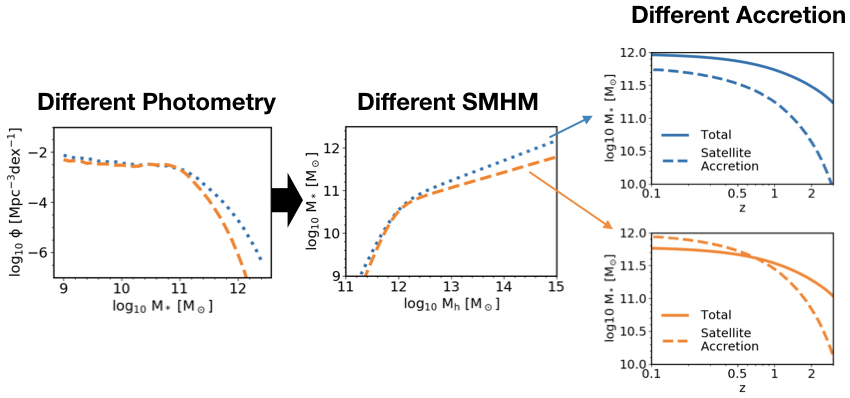
\includegraphics[width = \linewidth]{Figures/Chapter4/SMFtoAccretion.jpeg}
    \caption{A cartoon showing the steps we follow to connect the differences found in the stellar mass function (left) and the changes in the SMHM relation (SMHM, middle), that propagate into changes in the accretion histories (right). In the right hand panel dashed lines are mass from satellite accretion and solid lines are total galaxy mass growth. Flatter SMHM relations imply a weaker growth of stellar mass in the central which can be easily overcome by the substantial cumulative growth of merging satellites, rendering the model internally inconsistent.}
	\label{fig:SMFtoAcc}
\end{figure}

%cmodel
In Figure \ref{fig:SatelliteAccretioncMod} we show the satellite accretion generated using the `cmodel' SMHM relation/SMF given in Section \ref{C2:SubSec:AbnMtch}. 
The top row of  shows the total mass of the galaxy and the total contributed by satellite accretion. The middle row shows the fractional contribution from satellite accretion from $z = 3$. The bottom row shows the instantaneous mass growth from satellite accretion. In Figure \ref{fig:SatelliteAccretioncMod} we obtain a lower limit for the accretion rate by including stripping but not star-formation in the satellites thus minimizing their mass through environmental processes. We find for the high mass galaxies, which are above the knee of the SMHM relation, even the lower limit for the accretion has an instantaneous rate greater than the growth rate of the galaxy as seen in the bottom row. This makes the cmodel SMHM relation used within our dark matter accretion model \textit{non-physical}.

\begin{figure*}[h]
	\centering
	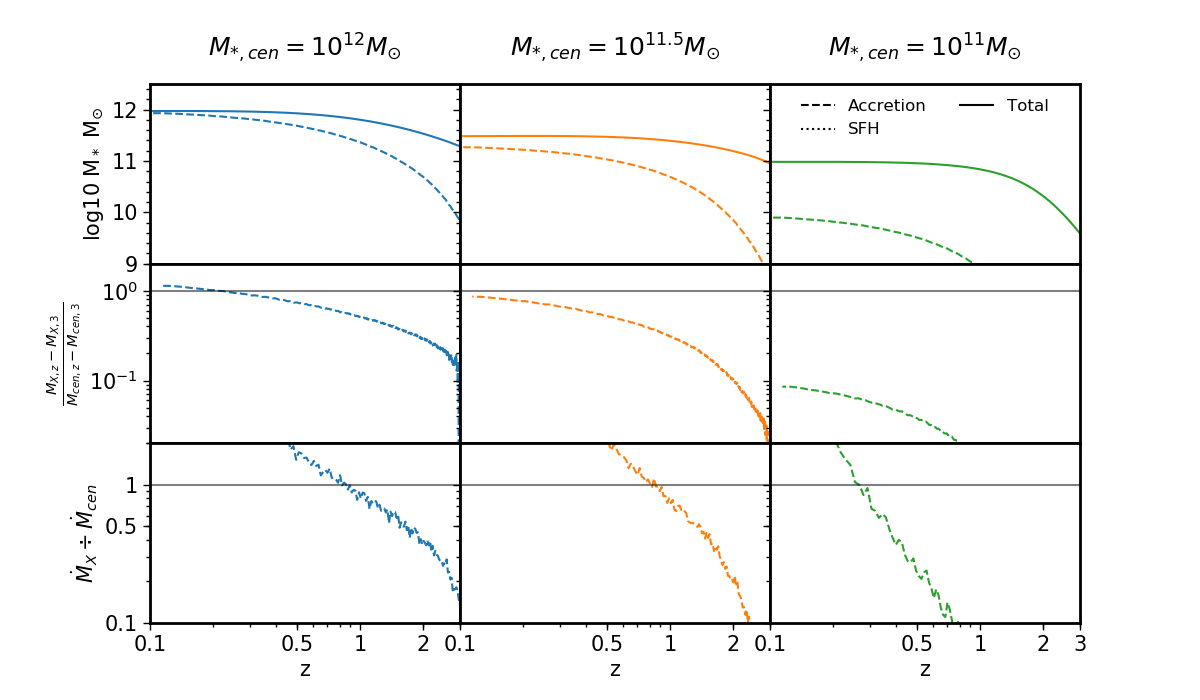
\includegraphics[width = \linewidth]{Figures/Chapter4/SatelliteAccretion_cMod.png}
    \caption{Three `mass tracks' are shown that have central galaxy masses at redshift $z = 0.1$ of $M_{*,cen}$ = $10^{12}$, $10^{11.5}$, and $10^{11}$ $[M_{\odot}]$ in blue orange and green respectively. It is clear that this model is internally nonphysical as the accretion via satellites (dashed lines) rapidly overshoots the total growth in stellar mass (solid lines) implied by the underlying growth host halo growth, as evident in the middle and bottom rows.}
	\label{fig:SatelliteAccretioncMod}
\end{figure*}

%pymorph
Similarly, the relative contributions to the average stellar mass growth of central galaxies from satellites and star formation history are calculated from \textsc{steel}, using the PyMorph SMHM relation/SMF given in Section \ref{C2:SubSec:AbnMtch}. This is shown in Figure \ref{fig:SatelliteAccretion} for three galaxy mass bins ($10^{11}$,$10^{11.5}$,$10^{12}$ $M_{\odot}$) selected at $z = 0.1$, the average growth history (total, solid lines) is derived by following the host halo-mass track, and the stellar-mass track is implied by imposing abundance matching at all redshifts. The stellar mass history assigned by abundance matching, is naturally independent of any galaxy merger modelling assumptions from \textsc{steel}. The total accretion from satellites (accretion, dashed lines) is computed from the expected satellite accretion along halo mass tracks. For each galaxy a star formation history (SFH, dotted lines) may then be calculated. The star formation rate is tuned such that it provides the correct star formation history to account for the difference between the mass growth expected from abundance matching and the cumulative satellite stellar mass accretion, the method for this is explained in detail in Section \ref{sec:SFR_Dev}.

\begin{figure}[h]
	\centering
	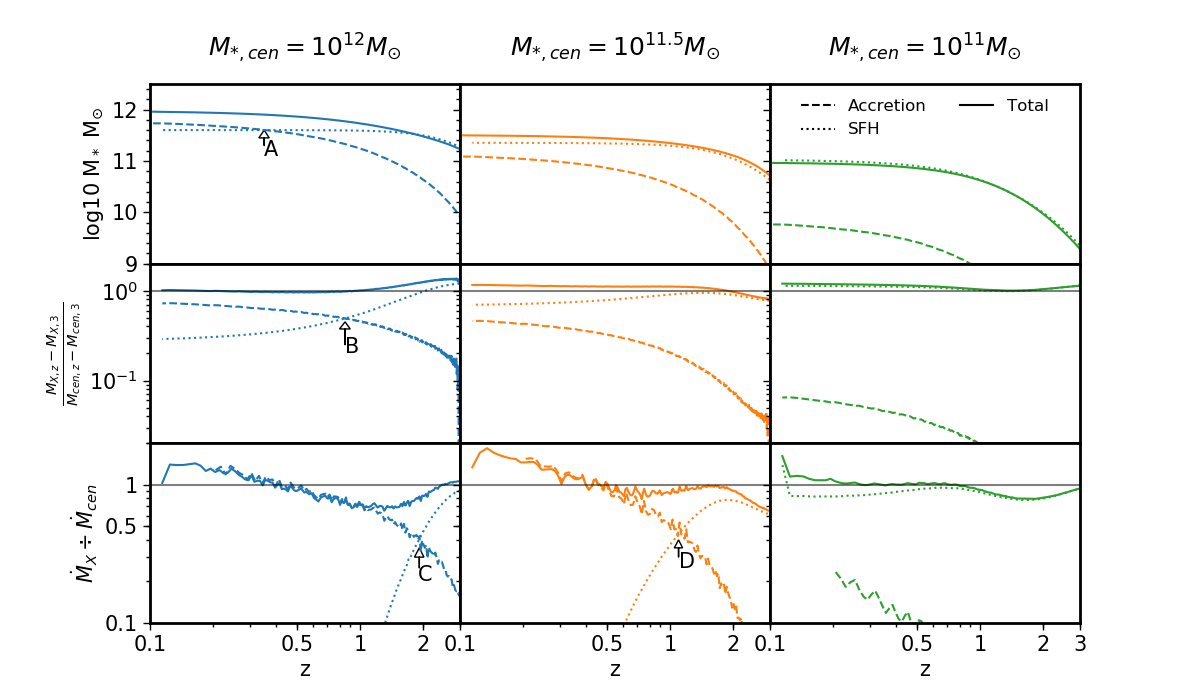
\includegraphics[width = \linewidth]{Figures/Chapter4/SatelliteAccretion_G19.png}
    \caption{Three `mass tracks' are shown that have central galaxy masses at redshift $z = 0.1$ of $M_{*,cen}$ = $10^{12}$, $10^{11.5}$, and $10^{11}$ $[M_{\odot}]$ in blue orange and green respectively. The satellite galaxy accretion is shown for evolved satellites with a dashed line, and the mass from star formation shown with a dotted line. The top panels show the total mass of the central (solid lines) and the total mass gained from accretion or star formation. The middle panels show the fraction of the total galaxy mass formed from satellite accretion or star formation since redshift $z=3$. The bottom panels show the ratio of the mass accretion rate from satellite galaxies, the star formation rate, and the mass growth rate of the central galaxy predicted by abundance matching. The black horizontal lines in the second and third rows are at unity. The solid lines showing the sum of the other two factors should be close to or on the unity lines. The labels A \& B point to where the cumulative mass from accretion overtakes the cumulative mass from star formation. The labels C \& D point to where the instantaneous accretion overtakes the star formation rate.}
	\label{fig:SatelliteAccretion}
\end{figure}

In Figure \ref{fig:SatelliteAccretion} we identify the epoch after which a galaxy transitions into a merger-dominated state under two definitions. Firstly, we define the ``cumulative transition'' as when the galaxy has accreted more mass than it has created from star-formation processes (Points A \& B). Secondly, we define the ``instantaneous transition'' as  the epoch when the growth rate from mergers overtakes the growth rate from star-formation (Points C \& D). More massive galaxies transition earlier to merger dominated growth under both definitions. However, all galaxies transition earlier under the second (instantaneous) definition. The masses shown in Figure \ref{fig:SatelliteAccretion} show three cases of relevant galaxy accretion tracks. The $M^{z=0}_* = 10^{12} M_{\odot}$ galaxy growth curve at low redshift is always dominated by satellite accretion. In the top and middle rows we see that more mass has been accreted than produced by star formation, and in the bottom row we see the accretion rate overtook the star formation rate at redshift $z=2$. The $M^{z=0}_* = 10^{11.5} M_{\odot}$ galaxy growth curve has more mass created from star formation than satellite accretion. However, the galaxy population has a higher rate of accretion rate than star formation rate since redshift $z = 1$. The final population shown at $M^{z=0}_* = 10^{11} M_{\odot}$ is star formation dominated under both cumulative and instantaneous definitions. At redshift $z = 0$ we find the transition masses for the total mass ratio and the instantaneous ratio to be at $M_* = 10^{11.7} M_{\odot}$ and $M_* = 10^{11.1} M_{\odot}$ respectively.

\section{Deriving the Star Formation Rate}
\label{sec:SFR_Dev}

The cartoon in Figure \ref{fig:SFRDerevation_Cartoon} shows the processes we follow to derive the star formation rate by following galaxy populations along their halo mass histories.\footnote{The coloured text is matched to the colours in Figure \ref{fig:SFRDerevation_Cartoon} intended to guide the reader though the multi-step process.} \textcolor{MPLgreen}{The plot labelled 1 (green) is the input stellar mass function.} \textcolor{MPLred}{The box in red is the statistical dark matter accretion history described in Section \ref{subsec:SDMAH}, including the halo mass function (2a), the central growth histories (2b), and the halo substructure (2c) shown here as a discrete merger tree for visualization purposes.} Using the abundance matching routines described in Section \ref{C2:SubSec:AbnMtch}, the \textcolor{MPLgreen}{stellar mass function (1)} and the \textcolor{MPLred}{halo mass function (2a)} are used to create the SMHM relationship (3, black).


In Chapter \ref{Chapter:GalDist} we showed how the \textcolor{MPLred}{dark matter accretion histories (2)} and abundance matching (3) can be used to generate \textcolor{MPLblue}{distributions of satellites for any central halo at multiple redshifts (4)}. For each \textcolor{MPLred}{central halo mass track (2b)} we calculate the average number density of satellites that reach the centre of the halo and merge with the central galaxy \textcolor{MPLblue}{thus generating the average satellite accretion history (dashed line, 5)}. \textcolor{MPLred}{Using the central halo growth histories (2b)} and the SMHM relation (3), we can generate the \textcolor{MPLblue}{average central galaxy growth history (solid line, 5)}. These two quantities can be compared to check for self-consistency, as described above and shown in Figure \ref{fig:SMFtoAcc}. Where a self-consistent central growth and accretion history is found any deficit between the accreted mass and the growth history is attributed to \textcolor{MPLblue}{star formation rate (delta, 5)}. \textcolor{MPLblue}{The derived star formation rate for central galaxies (solid line, 6) is compared to observational data (points, 6)}. Where the star formation rate prediction generated form the model is found to be consistent with observed star formation rates this is a good indication that the model is predicting correct accretion histories.

%Big Cartoon
\begin{figure}[h]
	\centering
	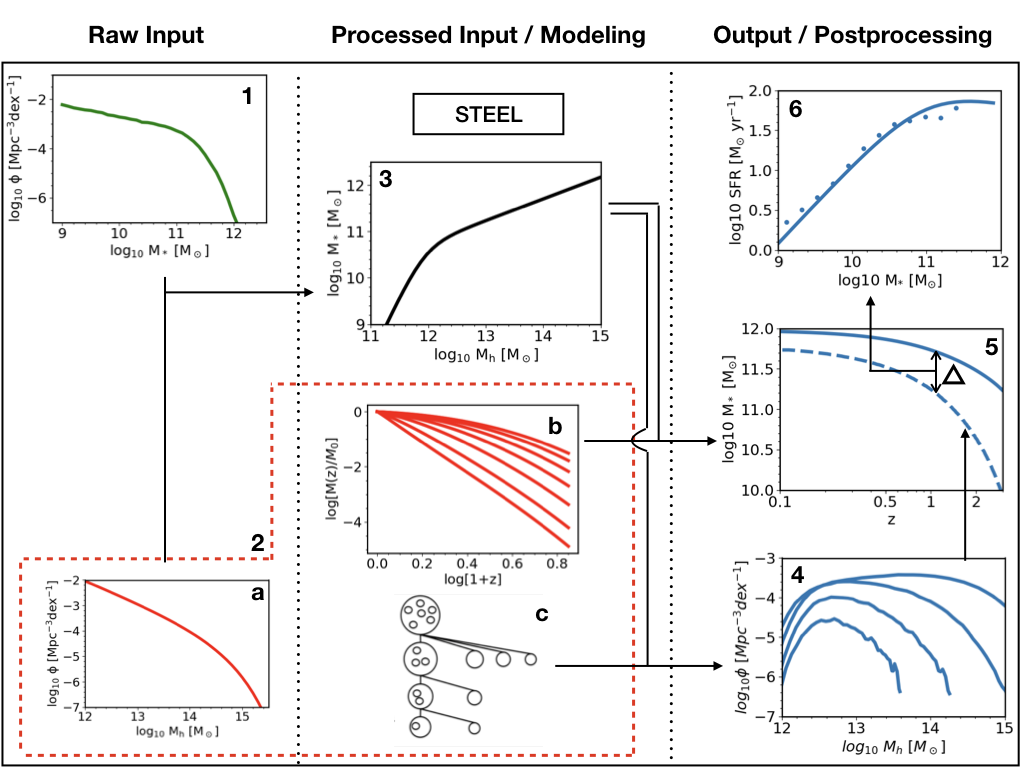
\includegraphics[width = \linewidth]{Figures/Chapter4/SFRFullCartoon.png}
    \caption{A cartoon showing the constituent steps of the method to generate star formation rates. In brief, the three columns from left to right are raw inputs, derived inputs/modelling, and output/post-processing. The subplots are: 1. The stellar mass function, 2a. The halo mass function, 2b. Halo mass growth histories, 2c. Accretion histories/Merger tree, 3. The SMHM relation, 4. Group/Cluster satellite richness, 5. Central growth histories/satellite accretion histories, 6. Star formation rate. The star formation rates are derived from the difference between the total growth in stellar mass and that from satellite accretion (panel 5).}
	\label{fig:SFRDerevation_Cartoon}
\end{figure}

The method described above directly links the star formation rate to the accreted mass from satellites. However, in our model satellites grow in mass after infall, we therefore must recalculate the full satellite accretion onto the central galaxies updating their mass using the new star formation rate. Using the updated accretion the star formation rate is recalculated beginning an iterative process. However, this iterative process of recalculation ends after one loop as the re-derived accretion is found to be nearly identical, as expected from the results of Chapter \ref{Chapter:GalDist}. When calculating this difference we also take into account the stellar mass loss rate (MLR) due to stellar recycling using Equations \ref{eqn:f_ml} \& \ref{eqn:MLR}. The star formation rate - stellar mass relation derived from this method is fit with a double power law that evolves with redshift given by the following Equation \ref{eqn:SFR_DPL},
\begin{equation}
\label{eqn:SFR_DPL}
\begin{split}
SFR(M_*, z) &= 2N(z)\Big[ \Big( \frac{M_*}{M_{n}(z)}\Big) ^{- \alpha(z)} + \Big( \frac{M_*}{M_{n}(z)}\Big)^{\beta(z)} \Big ]^{-1}\\
\log_{10} N(z) &= 10.65 + 0.33z - 0.08z^2\\
\log_{10} M_{n}(z) &= 0.69 + 0.71*z - 0.088z^2\\
\alpha(z) &= 1.0 - 0.022z + 0.009z^2\\
\beta(z) &= 1.8 - 1.0*z - 0.1z^2.
\end{split}
\end{equation}

\begin{figure}[h]
	\centering
	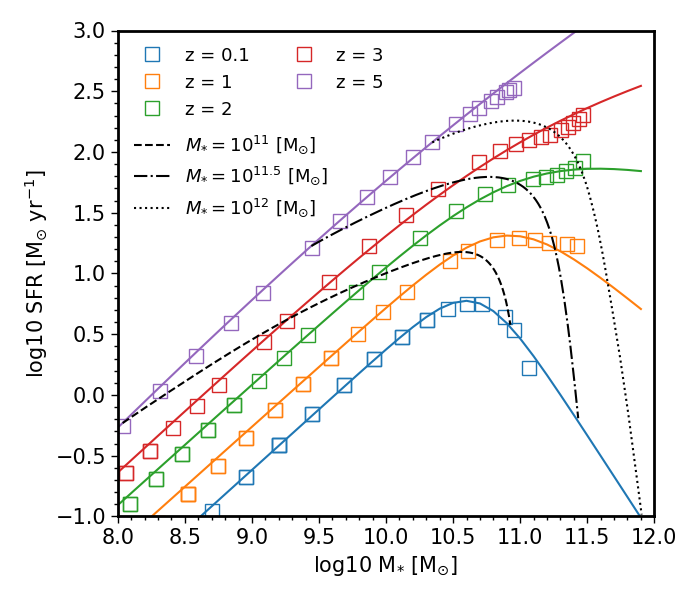
\includegraphics[width = 0.8\linewidth]{Figures/Chapter4/HMC_DPL.png}
    \caption{The star formation rate - stellar mass relation derived from following central galaxy populations along halo mass histories at redshifts $z = 0.1, 1, 2, 3, 5$. The data extracted from the post-processing of \textsc{steel} are shown by coloured crosses and the double power-law fits are shown as lines in corresponding colours. The three black lines are the evolution of the galaxy populations selected at redshift $z=0.1$ with masses $M_* = 10^{11}, 10^{11.5}, 10^{12} [M_{\odot}]$  presented in Figure \ref{fig:SatelliteAccretion}.}
	\label{fig:SFR_DPL}
\end{figure}

This fit (solid lines) to the computed SFR (open squares) is shown in Figure \ref{fig:SFR_DPL}. When visualised the general trend of the SFR is at lower redshift: the normalisation decreases, the peak of the distribution shifts to lower masses, and the turnover after the peak is steeper. We also show the same three galaxy population tracks from Figure \ref{fig:SatelliteAccretion} as black lines. These tracks show how the galaxy population evolves in SFR with redshift. The population tracks show a gradual increase in SFR and then a turnover before dropping sharply, as they transition to an ex-situ satellite accretion-dominated regime. It is found that smaller galaxies grow for longer timescales with increasing star formation, whilst larger galaxies start with higher star formation rate and transition to an accretion-dominated phase much earlier in time.

%Match to panchromatic data
\begin{figure}[h]
	\centering
	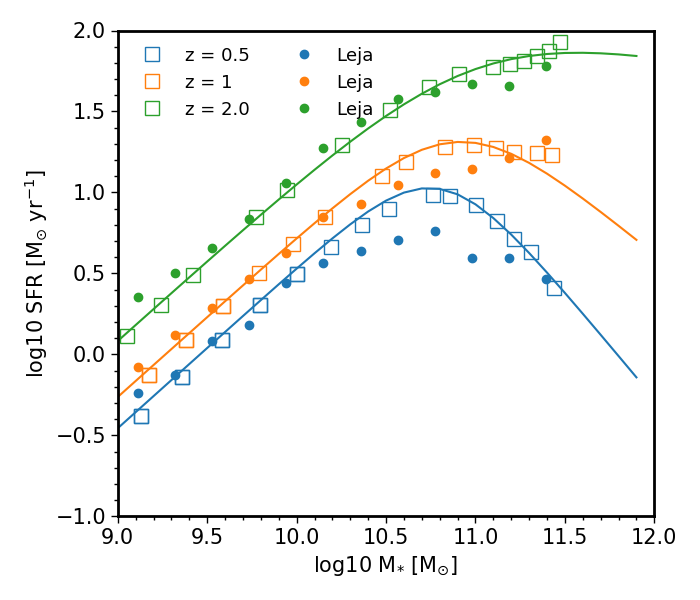
\includegraphics[width = 0.8\linewidth]{Figures/Chapter4/HMC_DPL_wLeja.png}
    \caption{I show the star formation rate - stellar mass relationship from Figure \ref{fig:SFR_DPL} at redshifts z = 0.5, 1, 2 (blue orange and green respectively, \textsc{steel} data are crosses and fits are solid lines). In this plot we compare with the observed star formation rate from \citet{Leja2019AnSurvey} shown as filled circles with corresponding colours denoting corresponding redshift.}
	\label{fig:SFR_L18}
\end{figure}

Recent work, where the star formation histories are properly accounted for when measuring star formation rates, has suggested that the previous determinations of star formation rates using UV+IR are 0.1 to 1 dex too high \citep{Leja2019AnSurvey} and cannot be reconciled with the growth of the stellar mass function \citep{Leja2015ReconcilingFunction, Lapi2017StellarEquation}. Our star formation rate is consistent with the results of \citet{Leja2019AnSurvey}, as reported in Figure \ref{fig:SFR_L18}. The excellent match to Leja et. al.'s independent estimates further supports the idea that a more robust method to derive more reliable star formation rates is to follow galaxy assembly along host halo growth histories \citep[see e.g.,][]{Moster2018Emerge10}. 

\subsection{Specific Star Formation Rate Distribution}
\label{subsec:sSFR}

Figure \ref{fig:sSFR} shows the specific star formation rate distribution of satellites in three mass ranges, as labelled, chosen to probe transitions found in observational data \citep{Bernardi2011EvidenceRelations, Bernardi2014SystematicMorphology, Cappellari2013TheFunction}. The solid blue line and the dashed black lines show the satellite and central sSFR from \textsc{steel}, respectively, while the grey histogram shows the satellites from SDSS and the unfilled histogram shows the centrals in SDSS. 

\textsc{steel} accurately captures the key trends in the distributions, such as bimodality, which is seen in both the central and satellite populations. The central population below $M_{*} = 10^{10.5}$ [M$_{\odot}$] is mostly star-forming whereas the satellites show signs of quenching. In the intermediate-mass range a fraction of the centrals become quenched and the satellites show a strong quenching effect. In the highest mass range all galaxies show strong quenching features with little star-formation. Whilst still not an exact match to the SDSS distribution, we find that including a redshift dependence in the dynamical quenching provides a better fit than the model used in Paper \RomanNumeralCaps{1}. The central sSFR is calculated using the star formation rate presented in Figure \ref{fig:SFR_DPL}, which uses the PyMorph SMHM relation. Each central mass is assigned a star formation rate with a scatter of 0.2 dex. To account for the fraction of galaxies that are quenched via mergers at each stellar mass we modify the assigned star formation rates by setting a fraction of galaxies equal to the elliptical fraction to have a sSFR of $10^{-12}$ [$yr^{-1}$] with a scatter of 0.2 dex and in turn increase the star formation rate of the remaining galaxies to maintain the same average star formation rate for the population. This approach tests if mergers alone can account for the bimodality found in the central sSFR, the high mass centrals $ > 10^{11.3}$ [M$_{\odot}$], but produces an inadequate fit to the SDSS centrals at masses lower than $10^{10.5}$ [M$_{\odot}$]. The discrepancies in the location of the star-forming population are likely caused by the imperfect fit to observed SFR as seen in \ref{fig:SFR_L18} and the deficit of quenched galaxies in the lower mass cuts is likely due to causes of quenching that are not merger related (e.g., AGN feedback).

%How the quenching differs
\begin{figure}[h]
	\centering
	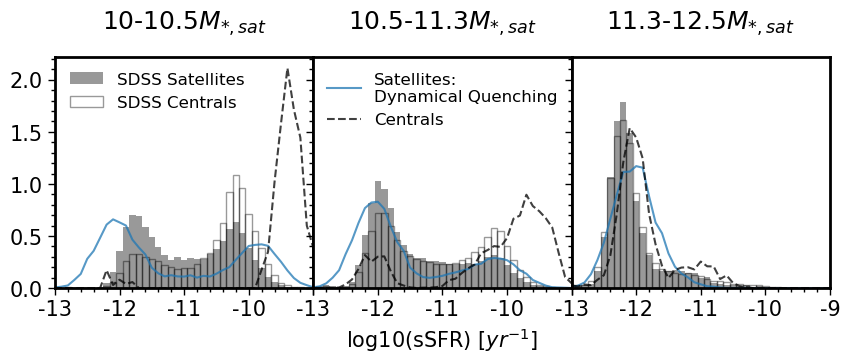
\includegraphics[width = \linewidth]{Figures/Chapter4/SSFR.png}
    \caption{We show the sSFR of satellites and centrals compared to SDSS in three mass bins selected to mirror proposed breaks in the galaxy main sequence. The SDSS data for satellites and centrals are filled and unfilled histograms respectively. The \textsc{steel} result for the satellites is the solid blue line and the post processed central result is the dashed black line.}
	\label{fig:sSFR}
\end{figure}

\section{Discussion}

In this chapter we found one of the major factors in regulating the in-situ and ex-situ accretion pathways to be the \textit{shape} of the SMHM relation. A shallower low-mass slope causes larger amounts of satellite accretion as smaller haloes, with much higher number density, are initialised with larger satellite galaxies. Similarly to \citet{Shankar2006NewFormation} \& \citet{Moster2018Emerge10}, we find the high mass slope to undergo only a small amount of evolution with increasing redshift, this implies the growth of central galaxies is directly linked to the steepness of the high mass slope and the growth of the host halo. The flatter the high mass slope of the SMHM relation, the less growth is expected in stellar mass following the assembly of the host dark matter halo. In turn, a weak evolution in the stellar mass content of the central galaxy can be in tension with what is expected from satellite accretion, especially for the most massive galaxies. We discussed that the slope of the high-mass end of the stellar mass function and implied slope of the SMHM relation strongly depend on the choice of light profile, background subtraction, and mass-to-light ratios. However, not all resulting stellar mass functions provide physically self-consistent results in a LCDM Universe. Steeper SMHM relations, such as those predicted by PyMorph-based stellar mass functions \citep{Bernardi2013TheProfile}, produce more consistent central and satellite accretion stellar mass growths. In addition to models with different SMHM slopes, we also tested models with the dynamical time varied by $\pm$20$\%$, within the range of possible dynamical times predicted in Chapter \ref{Chapter:GalDist} constrained by satellite richness. This relatively modest alteration has a minor effect on the satellite accretion rate and mass contribution to the central. In this work we find the transitional stellar mass, above which dry mergers progressively become the major contributor to galaxy growth, to be $M_{*} = 10^{11.1}$, see Figure \ref{fig:SatelliteAccretion}. The latter is consistent with previous findings \citep[e.g.,][]{Bernardi2011EvidenceRelations, Cappellari2013EffectEvolution, Shankar2013SizeUniverse}.


By following the statistical dark matter accretion histories we were able to use the central mass tracks and abundance matching to obtain a growth history for central galaxies. Subtracting from the latter at each time step the cumulative stellar mass from satellite accretion, we created a `star formation rate' interpreted as the remaining mass required to build the central mass. Our methodology is similar to the continuity approach based on \citet{Leja2015ReconcilingFunction} used in Paper \RomanNumeralCaps{1}, but with the key difference that here we follow halo growth instead of galaxy number density. 
The resulting star formation rate for galaxies is notably different to that of \citet{Tomczak2014GALAXY}, used in \citet{Grylls2019PredictingSteel.}. At all redshifts the turnover is notably different, with SFR for masses above the turnover decreasing sharply at low redshift. For masses below the turnover, at $z < 1$ the SFR is lower by 0.3 dex, and at $z > 1$ the SFR is higher by 0.1-0.2 dex. Additionally the SFR found from this method when combined with morphological quenching arguments reproduces well the bi-modality trends found in sSFR.

\subsection{Relation to effects in other models}

In this chapter we show that commonly used stellar mass function that have been accepted by the community and modellers are inconsistent with \LCDM cosmological models. The implications of this statement are of interest to wide reaching areas of galaxy modelling. 
\begin{itemize}
    \item \textbf{Distribution of satellites in semi-analytic models.} It has been shown \citep[e.g.][]{Asquith2018CosmicModels} that semi-analytic models struggle to reproduce the galaxy mass function at higher redshifts. At the masses shown this influences both the central and satellite populations. By fitting to a mass function that is not consistent with \LCDM assembly (even when excluding star formation) semi-analytic models must change their accretion histories to compensate. This is a potential explanation as why the 'best fit' models choose to break the less well constrained SMF at higher redshift.
    \item \textbf{Feedback, feedback, feedback.} Galaxy formation models (semi-analytic and hydro-dynamical) rely on a large amount of feedback, i.e. the processes that grow galaxies also lead to suppression of galaxy growth. The two feedback mechanisms that dominate the discussion of stellar mass growth are super-nova (SN) and active galactic nuclei (AGN), each of these have a large potential energy budget and therefore are excellent ways to reduce the efficiency of starformation. Largely these feedback routines are invoked over two different mass ranges as can be seen on the SMHM relation. SN decrease the efficiency of forming stars in the low mass regime by heating and ejecting gas in/from star-forming regions. In the high mass regime AGN are thought to eject energy over galaxy/halo scales suppressing starformation globally and quenching galaxies. The knee of the SMHM relation is then the point at which starformation has been most efficient as the sum of these process has least effect. However, AGN feedback according to many studies and the AGN modelling community (as opposed to the galactic modelling community), may not be able to couple as efficiently as required in galaxy modelling. If AGN were to be less efficient at quenching then the result would be an increase in the SMHM relation high mass slope as we find in our best fit model. It follows that the aggressive feedback found to be required in galaxy modelling is actually a result of trying to suppress star formation to reduce the mass budget from starformation to allow for more of this budget to come from accretion to better fit SMF that do not match cosmological models.
    \item \textbf{Illustris TNG high mass slope.} In Figure \ref{fig:Abn_Data} we show the SMHM relation from the Illustris TNG \citep{Nelson2018TheRelease}. It can be seen that the high mass slope is significantly higher than even that produced using the PyMorph SMF. Where Illustris focuses on the reproduction of galaxy structure, formation, and clustering, above reproduction of the SMHM relation or SMF the high mass slope naturally steepens as is the consequence of the hierarchical assembly as put forward in this chapter.
\end{itemize}


\section{Conclusions}

It is important to note that whilst the discussion and analysis of how this incompatibility with other modelling techniques could be interpreted to show that any combination of \LCDM theories, stellar mass functions, galaxy feedback, e.t.c, could be wrong. This would however be a needlessly adversarial exercise, the results presented are better thought of as a guideline for the scope of what any model can predict. A result, such as presented that focuses on the reproduction of satellites and central growth is by design appropriate to investigate in-situ vs ex-situ growth whilst forgoing any direct feedback modelling, whereas, a model such as illustrious is appropriate to look at how physical processes shape the formation of galaxy sizes, morphologies e.t.c. The goal for a holistic cosmological model of galaxy formation is an important endpoint and understanding the scale of simulation required to do this is essential. For example simulating starformation in a hydro-dynamical simulation is done by averages temperatures densities and pressure in large cells, as starformation is a nuclear physics process we are necessarily smoothing over effects that may effect the results. In n-body dark matter simulations the force softening parameter that is designed to allows averaging over many particles has been show to effect the subhalo breakdown and accretion \cite{vandenBosch2018DisruptionFiction}. Each of these provide examples as to compromises that prohibit a `full' simulation of galactic cosmology. This chapter shows not that the observations or the \LCDM cosmology is wrong but more that each prediction was made without the other in mind and there core assumptions are in some what incompatible. Cosmological models of galaxy formation that cannot work from first principles must begin and end with a clear question to answer such to generate predictions. Where more than one theoretical or observational data-set is used the axioms implicit to the observation must be understood to ensure the self consistency and limits that must be observed when reporting results.

\subsubsection{Future work}
The work presented in this chapter, checking self consistency between \LCDM halo assemblies and stellar mass functions has one application that appears more critical than others. If this consistency checking can be refined, and turned into a pipeline, then it can be integrated into data analysis pipelines that make stellar mass determinations using several models under flexible cosmological parameters. Each stellar mass estimation model can then be associated with a set of cosmological models and vice versa, equally stellar mass estimations and cosmological models that do not find matches can be discarded. The primary drawback of such a technique would be that it wouldn't take account of the evolution of galaxies only the masses as assigned by abundance matching. 

To improve the abilities of an integrated method additional empirical modelling can be performed such as the starformation derivation in this chapter, the satellite distributions and pair-fractions presented in Chapters \ref{Chapter:GalDist} \& \ref{Chapter:GalPairs}, or the morphologies from Chapter \ref{Chapter:GalPairs}. With these and other such constraints empirical models can be built that reproduce all observables intended to be drawn from a survey. In this way all assumptions made in estimating galaxy features from a survey such as initial mass function, light profile, star-formation rate e.t.c can be checked at point of derivation to avoid the inconsistency issues that have thus far been systemic\footnote{As discussed: \begin{itemize}
    \item SMF and SFR continuity.
    \item Stellar mass estimation and \LCDM assembly
    \item Stellar mass estimation and pair fractions
\end{itemize}} in galaxy observations. 
 % Discuss how galaxies grow including how we can use this as a tool for scientific testing

% Chapter 5

\chapter{Galaxy Pairs, Mergers, and Morphologies} 
\label{Chapter:GalPairs}
\lhead{Chapter 5. \emph{Pairs, Mergers, and Morphologies}} 

\section{Background}

$\Lambda$CDM cosmology predicts the hierarchical assembly of dark matter haloes.
Throughout the history of the Universe haloes have grown in mass and size via two pathways. 
Firstly haloes grow via smooth accretion gradually accreting dark matter from the surrounding environment. 
The secondary growth mechanism is via the accretion and gradual absorption of smaller haloes, known as subhaloes. 
After accretion subhaloes survive as substructure of the central/host halo gradually losing mass and sinking to the center of the potential well though dynamical friction. As discussed in previous Chapters these sub-haloes contain satellite galaxies that follow the halo structure causing galaxy galaxy mergers.

Frequent or massive mergers are thought to induce morphological changes in galaxies. 
Galaxies, after experiencing a massive merger, where the minor galaxy is at least a quarter of the mass of the central galaxy, are thought to lose their disk-like morphology and transform into elliptical galaxies \citep{Negroponte1983SimulationsGalaxies, DeLucia2006TheGalaxies}. 
For this reason it is important to understand the frequency and nature of mergers between galaxies to achieve a complete and coherent picture of galaxy formation and evolution. 
Unfortunately, galaxy mergers occur on gigayear timescales and therefore it is not possible to directly observe the rate or consequence of galaxy mergers. 
The traditional approach to estimate a measure of galaxy mergers is to count galaxy pairs at a given separation, and then assign a merging timescale to infer the rate of galaxy merging \citep{Conselice2003A3,Conselice2008TheField,Mundy2017A3.5,Duncan2019ObservationalFields}.
However, the approach of counting pairs is complicated by systematic differences when selecting galaxies, for example the evolution of the pair fraction appears to change if a selection is made by flux ratio or made by stellar mass ratio \citep{Man2016RESOLVING03}.

\section{The systematic effects of stellar mass estimation on galaxy pair fractions}

%What systemeatics can we expect to find in galaxy pairs (paper 3 plots 1,2,&3)

In this chapter we show how different SMHM relations generate distinct pair fractions and merger rates. 
Stellar mass functions with greater number densities of high-mass galaxies, naturally map larger galaxies into smaller haloes due to their higher relative abundances, resulting in steeper high-mass slopes for the SMHM relations.
In Figure \ref{fig:MassRatioCartoon} we show an illustrative cartoon of how different SMHM relations affect the galaxy mass ratios. 
For two identical mass halo pairs we see that a SMHM relation with a steeper slope causes a substantial difference in the stellar mass ratio that is mapped into the halo pairs. 

\begin{figure}[h]
	\centering
	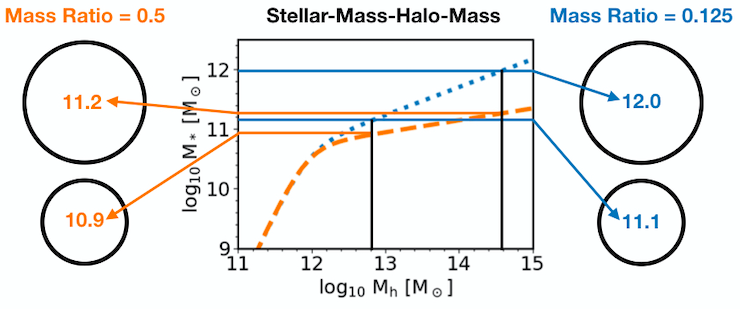
\includegraphics[width = \linewidth]{Figures/Chapter5/MassRatioCartoon.png}
	\caption{A cartoon showing the how the SMHM relation can impact the stellar mass ratio of galaxies mapped into identical halos. The steeper SMHM relation creates a smaller stellar mass ratio as the change in halo mass maps to a much larger stellar mass difference.}
	\label{fig:MassRatioCartoon}
\end{figure}

It follows that given two identical distributions of haloes seeded with galaxies via different SMHM relations the shallower one will seed more galaxy pairs\footnote{The pair fraction  defined here as the fraction of galaxies of a given mass that have a companion with a mass equal to or greater than a quarter of the primaries mass within 5-30 kpc.}.

In Figure \ref{fig:SMHM_PF_Cartoon} a cartoon is shown as an example of the expected difference in the pair fraction when changing the SMHM relation.
The left hand column shows the SMHM relations and the right column the pair fractions and their evolution with redshift. 
In the top row we compare a steep high-mass slope to a flatter slope, where the slope has been changed at redshift $z = 0.1$.
In the bottom row we compare an evolving and non-evolving high-mass slope.

\begin{figure}[h]
	\centering
	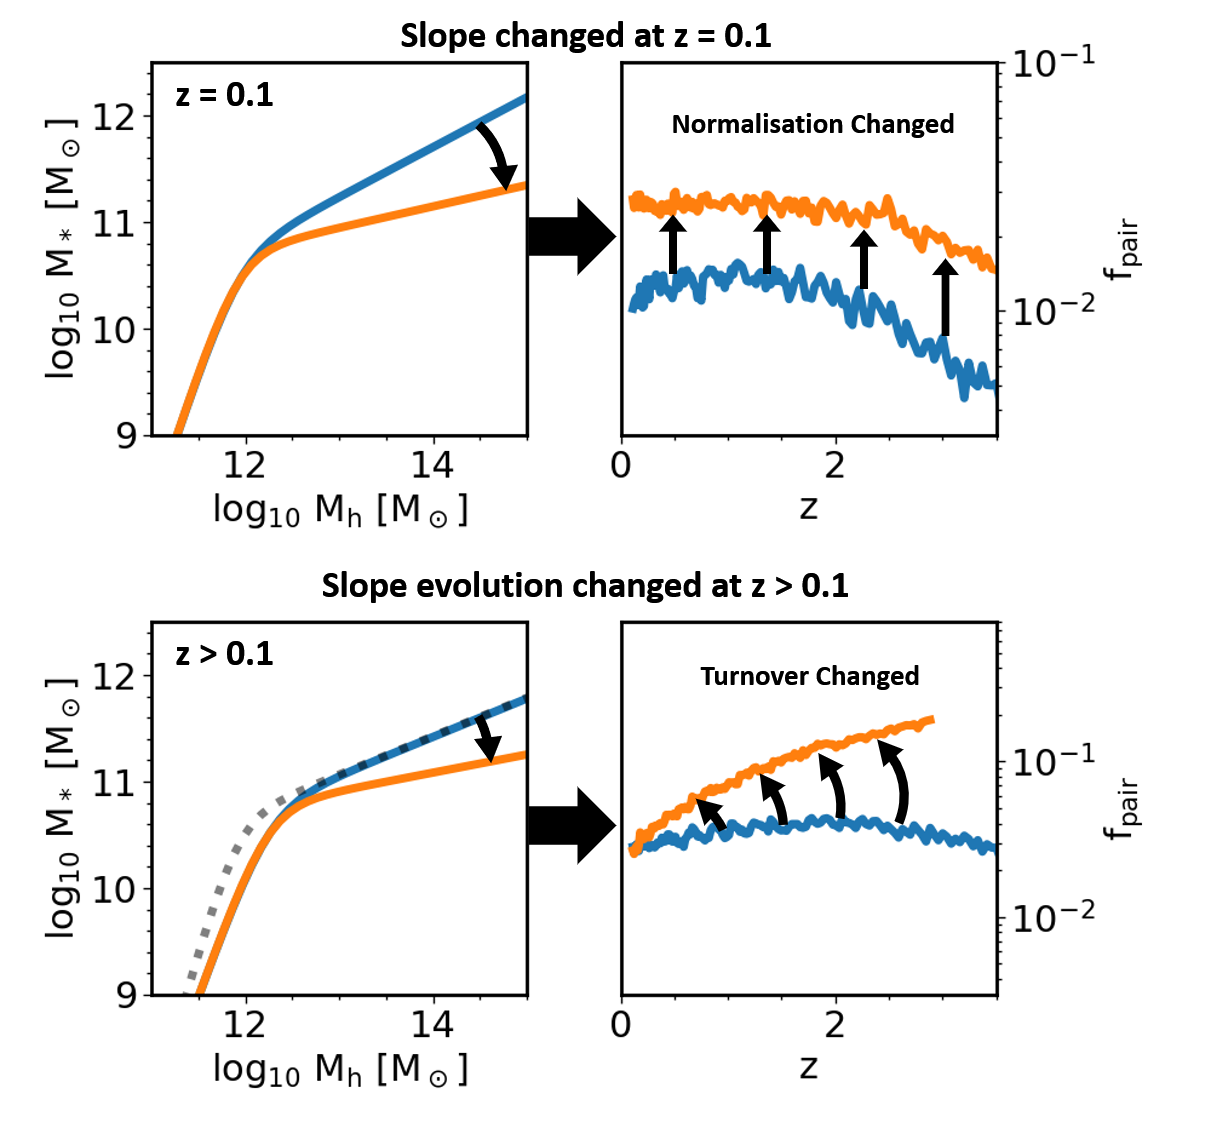
\includegraphics[width = \linewidth]{Figures/Chapter5/SMHM_PF_Cartoon.png}
	\caption{A cartoon showing the how the SMHM relation can impact the pair fraction. The top row shows how reducing the high mass slope of the SMHM relation increase the number of pairs at all redshifts. The bottom row shows the redshift $z=0$ relation as a grey dotted line, two relations at redshift where the relation is not evolved or evolved to be shallower are shown in blue and orange respectively. For this evolving SMHM relation the pair fractions are found to increase. In each case the reason for the increase can be explained by referencing Figure \ref{fig:MassRatioCartoon} where making the relation shallower seeds more massive pairs.}
	\label{fig:SMHM_PF_Cartoon}
\end{figure}

The steepening of the SMHM relation high-mass slope increases the number of pairs created and the normalisation of the pair fraction increases. 
In the bottom row we show the effects of having a slope that flattens at higher redshift. 
We show the redshift $z=0.1$ relation in grey and the relations with the unchanged and changed slopes in blue and orange respectively. 
The main effect of varying the evolution of the high-mass slope in the SMHM relation is to change the behaviour of pair fraction with redshift. 
A steeper slope tends to turn over the pair fraction and vice-versa.


The behaviours reported in Figure \ref{fig:SMHM_PF_Cartoon} are what one would expect given Figure \ref{fig:MassRatioCartoon}, where shallower slopes give higher fractions. 
Furthermore, from Figure \ref{fig:SMHM_PF_Cartoon} (and from Figure \ref{fig:PairFracSystematic}), it can be concluded that almost any pair fraction difference could be produced by appropriately altering the input SMHM relation. 
It is relevant to stress here that relatively minor changes in the stellar mass function can cause qualitative differences in the SMHM relation and, by extension, in the shape and normalization of pair fractions at any cosmic epoch.

The ability to systematically change the pair fraction due to stellar mass derivation calls to question the discrepancies found in pair fraction results \citep[e.g.][]{Man2016RESOLVING03}. 
If the pair fraction is systematically effected then where results do not use the same data processing then the difference could be due to non-trivial systematics. 
\steel as a flexible and lightweight model can illuminate the systematics by running with multiple input SMHM relations to test a range of different inputs and compare the results.

Calculation of the pair fraction in \steel requires an estimate of the distance between the central galaxy and the satellite galaxy, as we rely on our statistical accretion history, and do not have discrete halos, we assign each subhalo bin an average distance to the central galaxy. 
The subhaloes start at the viral radius of the central halo, the distance to the centre then reduces proportionally to the amount of dynamical time remaining \citep{Guo2011FromCosmology}.

To generate the systematic outputs a toy model where each of the main parameters (M, N, $\beta$, $\gamma$), and their evolutionary factors (M$_z$, N$_z$, $\beta_z$, $\gamma_z$), governing the SMHM relation are adjusted in turn to explore the affect on the galaxy pair fractions. Table \ref{tab:PairFracSysInput} details the change made to the SMHM relation for each parameter. 

\begin{table}
\centering
\caption{The adjustments to the SMHM relation used in Figure \ref{fig:PairFracSystematic}.}
\label{tab:PairFracSysInput}
\begin{tabular}{|c|cccc|} \hline
             & PyMorph   & $X_{0.1, alt}$  & $X_{z, +}$  & $X_{z, -}$  \\ \hline
$M$          & 11.92 & -0.25 & -     & -     \\ 
$M_{z}$      & 0.58   & -     & +0.1  & -0.1  \\ \hline
$N$          & 0.032 & +0.04 & -     & -     \\
$N_{z}$      & -0.014 & -     & +0.007 & -0.007 \\ \hline
$\beta$      & 1.64  & -0.3  & -     & -     \\
$\beta_{z}$  & -0.69  & -     & +0.3  & -0.3  \\ \hline
$\gamma$     & 0.53  & +0.06 & -     & -     \\
$\gamma_{z}$ & -0.03  & -     & +0.2  & -0.2  \\ \hline
\end{tabular}
\end{table}

Figure \ref{fig:PairFracSystematic} shows each of the SMHM relations in the outer four panels, the reference SMHM relation PyMorph is shown in blue at redshifts $z = 0.1$ (dotted line) and $z = 2$ (dashed line) in each panel, the modified redshift $z = 0.1$ relation is then shown in orange, and the increased and decreased (dashed red and green) evolution are shown at redshift $z = 2$. The inner four panels follow the same colour convention. 

\begin{landscape}
\begingroup
\begin{figure}[h]
	\centering
	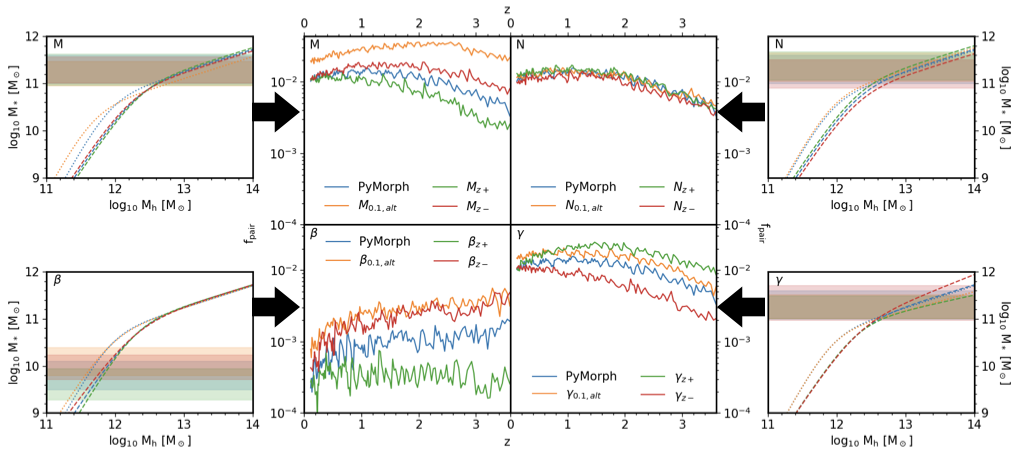
\includegraphics[width = \linewidth]{Figures/Chapter5/PairFractionSystematic.png}
	\caption{Each of the panel pairs (M, N, $\beta$, $\gamma$) shows the input SMHM relation in the outer plot and the modelled pair fraction evolution in the center plot. Each pair investigates adjustments to the given parameter of the SMHM relation (M, N, $\beta$, $\gamma$). Each pair shows the reference SMHM relation `G18' in blue, the relation adjusted at redshift $z = 0.1$ keeping the same SMHM relation evolution parameters in yellow. The red and green lines have the evolution parameter altered such that the evolution parameter is increased or decreased with respect to PyMorph respectively. In the outer (SMHM relation) plots dotted lines are $z = 0.1$ relations and dashed lines are $z = 2$ relations the PyMorph relation is shown at both epochs for comparison. Finally the shaded bands in the outer plots show the consistent number density selections used in the center plots.}
	\label{fig:PairFracSystematic}
\end{figure}
\endgroup
\end{landscape}

When changing M, the knee parameter, a large increase in the pair fraction is found from a lower knee: The shallower high mass slope is extended therefore more haloes are seeded in the mass range for pairs. 
We see the same effect at high redshift, the lower value of M at high redshift creates a higher pair fraction. 
The normalization parameter, N, creates little change in the pair fraction as expected because the mass ratios are largely unaffected. 
The low mass slope parameter, $\beta$, affects the seeding of smaller galaxies hence a lower mass range is used for the consistent number density cut. 
Due to the steepness of the low mass slope the fraction of pairs is lower in this mass cut.
Finally, when the high mass slope parameter, $\gamma$, is altered more pairs are found at high and low redshift when the slope is shallow. 
This is again attributed to more galaxies seeded within the mass ratio range.

\subsection{Simulation and Observational Results}
\label{subsec:SimObsRes}
The observed pair fraction is known to have discrepancies based on the galaxy property used to calculate the ratio. In \citet{Man2016RESOLVING03} it is shown that selecting pairs by flux ratio or stellar mass creates differences in the pair fraction evolution. 
In Figures \ref{fig:MassRatioCartoon} \& \ref{fig:SMHM_PF_Cartoon} we show the predicted effect of the determination of stellar mass on the SMHM relation and the propagation of these changes into the pair fraction. 
Through the use of a toy model in Figure \ref{fig:PairFracSystematic} we show how isolated perturbations to the eight SMHM relation parameters propagate into the galaxy pair fraction.
Given this analysis we find that any observation of the pair fraction must be understood in terms of its implicit observational assumptions. 
Furthermore, direct comparison of pair fraction results should only be undertaken under identical stellar mass derivation assumptions, where this is not the case the influence of any differences must be accounted for.
In this section we fit, by making use of $\steel$, observed pair fractions using small changes to the SMHM relation.
We anticipate this modelling can be used to provide corrections to pair fraction results to allow for fair comparisons.

In Figure \ref{fig:PairFractionIll} we show the simulated galaxy pair fractions for galaxies in the mass range $M_*$ = $10^{10}$ to $10^{10.6}$. The pair fraction is shown for two different SMHM relation inputs to $\steel$. In blue we show the PyMorph (S\`ersic Exponential) input used as the baseline in Figure \ref{fig:PairFracSystematic}, in orange the input calibrated to match the Illustris TNG simulation. In the right hand panel we see that the the prediction from \steel with the TNG-calibrated input is in good agreement to the pair fraction extracted directly from the Illustris TNG simulation. The pair fraction predicted using the PyMorph input is 0.5 dex lower, this is to be expected as in the mass range we are considering the Illustris TNG simulation SMHM relation is shallower and more pairs are therefore created in a greater mass range of halo mergers. 
\begin{figure*}
	\centering
	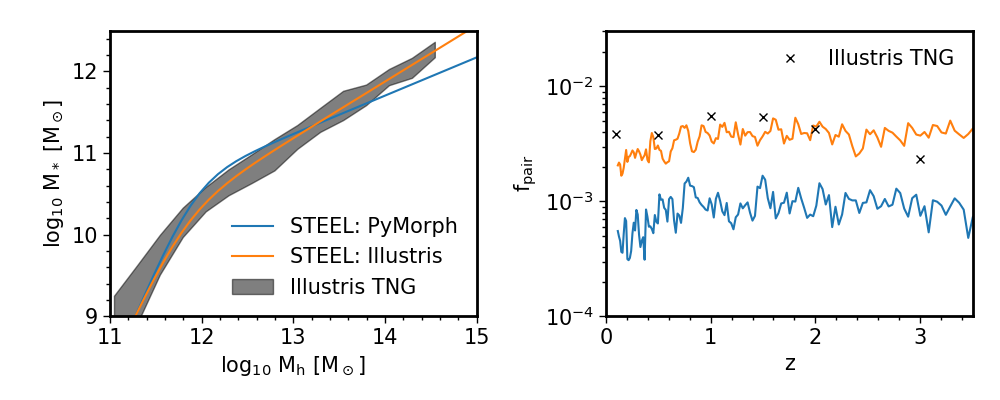
\includegraphics[width = \linewidth]{Figures/Chapter5/PairFractionIllustris.png}
    \caption{Left: Two SMHM relations are shown from \steel using parameters designed to reproduce the SMHM relation found in the Illustrius TNG simulation (Orange line) and the PyMorph(S\`ersic Exponential) fit parameters (Blue line). The shaded region is the output from the Illustris TNG simulation. Right: The pair fraction, for galaxies in the mass range $M_*$ = $10^{10}M_{\odot}$ to $10^{10.6}M_{\odot}$ generated from \steel is shown for runs using both the SMHM relations, lines follow the same colours as the left hand panel. The pair fraction extracted directly from the Illustris TNG simulation is shown using black crosses.}
	\label{fig:PairFractionIll}
\end{figure*}

Figure \ref{fig:PairFractionData} shows the predicted pair fraction evolution using the two SMHM relations from PyMorph and cmodel presented in Section \ref{subsec:SMHM}. The left panel shows each SMHM relation at redshift $z = 0.1$ and $z = 2.5$. Following the systematic investigation in Figure \ref{fig:PairFracSystematic} we attribute the 0.1 dex difference in pair fraction to the difference in high mass slope between PyMorph and cmodel. The best-fit relation from \citet{Mundy2017A3.5}, shown as black crosses, rises rather than falling as seen from PyMorph and cmodel. We see in Figure \ref{fig:PairFracSystematic} a SMHM relation with a high mass slope that decreases with redshift creating a pair fraction evolution of this nature.

\begin{figure*}
	\centering
	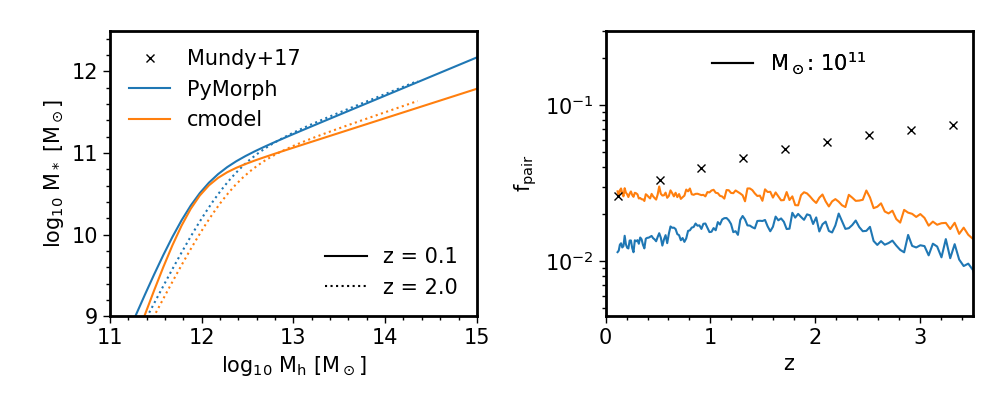
\includegraphics[width = \linewidth]{Figures/Chapter5/PairFractionData.png}
    \caption{Left: The stellar mass halo mass relations derived from PyMorph (blue) and cmodel (orange) at redshifts 0.1 (solid lines) and 2.0 (dotted lines). Right: The pair fraction evolution for galaxies using both SMHM relations. We make mass cuts, $>10^{10}M_{\odot}$ (dashed line) and $>10^{10}M_{\odot}$ (solid line), in PyMorph and cmodel. The black crosses show the corresponding best fits for the $>10^{11}M_{\odot}$ mass cut from \citet{Mundy2017A3.5}.}
	\label{fig:PairFractionData}
\end{figure*}

To attempt to match the \citet{Mundy2017A3.5} pair fractions we begin using the cmodel SMHM relation which gives the closest match in pair fraction at low redshift. Following the analysis of Figure \ref{fig:PairFracSystematic} where higher $\gamma_{z}$ increases the pair fraction at high redshift we alter the parameter from 0.0 to 0.5 in steps of 0.1. In Figure \ref{fig:PairFractionHMevo} the left panel shows the SMHM relation at redshift 0.1 as a black dotted line then coloured lines show the relation at redshift $z = 2$ given the different $\gamma_{z}$ parameters. The right panel shows the impact of this evolution on the pair fraction, as predicted higher $\gamma_{z}$ increases the pair fraction with redshift and a value of above 0.1 removes the turnover. Comparing to \citet{Mundy2017A3.5} we see a value of $\gamma_{z}$ between 0.1 and 0.2 best reproduces the rise in pair fraction. 

\begin{figure*}
	\centering
	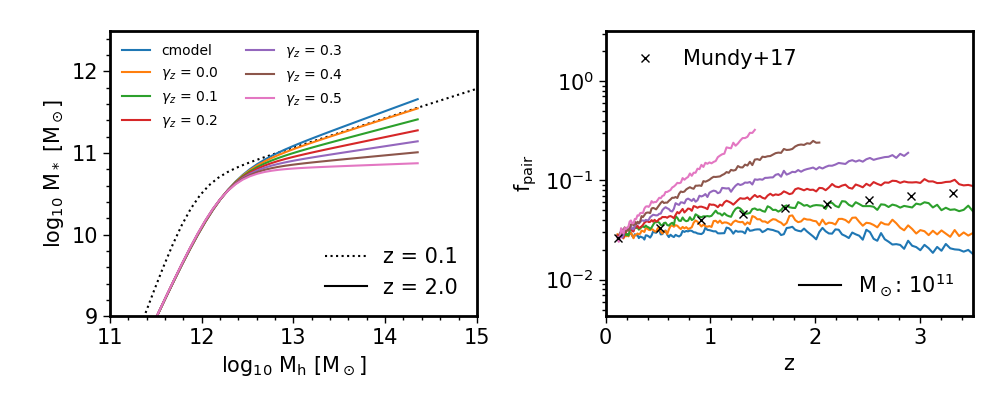
\includegraphics[width = \linewidth]{Figures/Chapter5/PairFractionHMevo.png}
    \caption{Left: The stellar mass halo mass relations derived from cmodel (black) at redshift $z = 0.1$ (dotted lines) and at $z = 2.0$ (coloured lines) with altered high mass slope evolution parameter. Right: The pair fraction evolution for galaxies each altered SMHM relation. The black crosses show the corresponding best fits for the $>10^{11}M_{\odot}$ mass cut from \citet{Mundy2017A3.5}.}
	\label{fig:PairFractionHMevo}
\end{figure*}

\section{Galaxy Morphologies Resulting from Galaxy Mergers}
%What happens during a galaxy merger?

Mergers are thought to be one of the drivers for morphological transformation, size growth and other galaxy changes \citep{Bournaud2007, Hopkins2009TheDemographics, Hopkins2010MergersFunctions, Shankar2011SizeUniverse, Fontanot2015OnMergers}. A number of analytically-based cosmological models have generally assumed that major mergers, in particular, with a mass ratio of at least $M_{sat}/M_{cen} > 0.25(to 0.3)$, are effective in destroying disks and in forming ellipticals \citep{Baugh2006AApproach, Malbon2007BlackFormation, Bower2010TheFormation}. However, galaxy mergers happen on timescales that dwarf human lifespans so when we observe galaxy mergers we essentially see a static snapshot of the process. Therefore, much of our knowledge of galaxy mergers then comes from simulations of merging systems \cite[e..g.][]{Hopkins2006ASpheroids,Hopkins2009TheDemographics, Hopkins2010MergersRate,Hopkins2009HOWMERGERS,Hopkins2010MERGERSMATTER,OLeary2020EMERGE:zsim6,Fensch2017High-redshiftFormation,Stewart2008MergerSurvival,Stewart2009GALAXYDEPENDENCE}. 

Despite this wealth of simulations of galaxy mergers, the fulcrum of our understanding lies with the estimation of the rate and significance of mergers \cite{Hopkins2010MERGERSMATTER, Hopkins2010MergersRate}. Using the merger rates derived in Chapter \ref{Chapter:GalGrowth} we implement a post-processing method to ascertain the effects of traditional models when decoupled from merger trees and applied to true, statistical, populations in \steel.

%The fraction of elliptical galaxies stemming from galaxy major merger in steel
\subsection{Implementing discrete processes in a statistical model.}

One of the primary challenges in the development of \steel is trying to implement discrete processes in a statistical fashion. Mergers that happen between two galaxies are implemented stochastically using the following method.
\begin{itemize}
    \item At each time-step for each central halo mass track the mass bins of previously accreted subhalo/satellite galaxy mass functions that have reached the end of their dynamical time are summed to produce the merging satellite stellar mass function. 
    \item Each central halo mass track is assigned a central stellar mass at each epoch $M_{*,cent}(M_{h}, z)$ (Figure \ref{fig:Cent_Mass_PP}). By integrating the merging satellite stellar mass function in the range [$M_{*,cent}(M_{h}, z) \cdot \mu$, $M_{*,cent}(M_{h}, z)$] the probability that a given central has undergone a major merger at each epoch is retrieved, where $\mu$ is the major merger mass ratio. 
    \item In Figure \ref{fig:Gal_Morph_toon} an illustration of the way galaxy morphologies are updated is given. 
    \begin{itemize}
        \item In the leftmost panel all galaxies are spirals or a disk like morphology (blue bar), the probability of a galaxy having a major merger is shown as a black line.
        \item Following the arrow to the middle panel the fraction of galaxies that had a major merger are assigned as ellipticals. The mass track at this epoch now has this spiral to elliptical ratio.
        \item At this next time step the fraction of galaxies undergoing a major merger is calculated, however, this is split between galaxies that have previously had a major merger and those that have not. 
        \item Following the arrow from the middle to the right hand panel we see only the galaxies that were in the spiral group contribute to the increased elliptical fraction.
        \item Using this process at each time-step eventually all galaxies can become elliptical but the rate at which this happens slows.
    \end{itemize}
    \item Using the process as described we can apply discrete processes to mass tracks that describe a diverse population.
\end{itemize}

\begin{figure}[h]
	\centering
	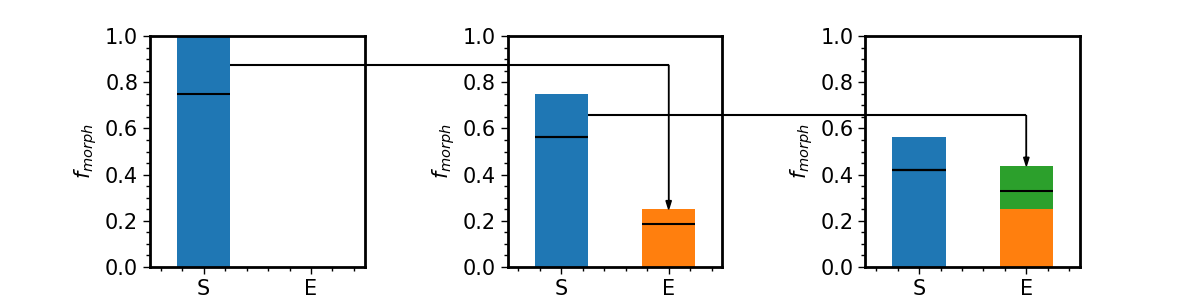
\includegraphics[width = \linewidth]{Figures/Chapter5/Morphology_Evolution.png}
	\caption{A cartoon of the way we assign morphologies statistically in $\steel$. Each step has the same fraction of major mergers but the number of ellipticals created reduces as some major mergers occur on the elliptical fraction. The fraction of galaxies in each population experiencing a major merger is displayed as a horizontal black line.}
	\label{fig:Gal_Morph_toon}
\end{figure}

Applying the above process to galaxies in \steel from redshift $z = 3$ we obtain the morphological fraction of galaxies at different masses using a major mass ratio of $\mu = 0.25$, at redshifts $z = 0.1, 0.65, 1.75$. Figure \ref{fig:Gal_Morph} shows the probability/fraction of central galaxies that have elliptical morphologies, while the black triangles show the T-Type-selected elliptical fraction from the SDSS catalogue. We find that applying this simple recipe to the merging number densities from \textsc{steel} creates a good match to the elliptical fraction in the local universe.

\begin{figure}[h]
	\centering
	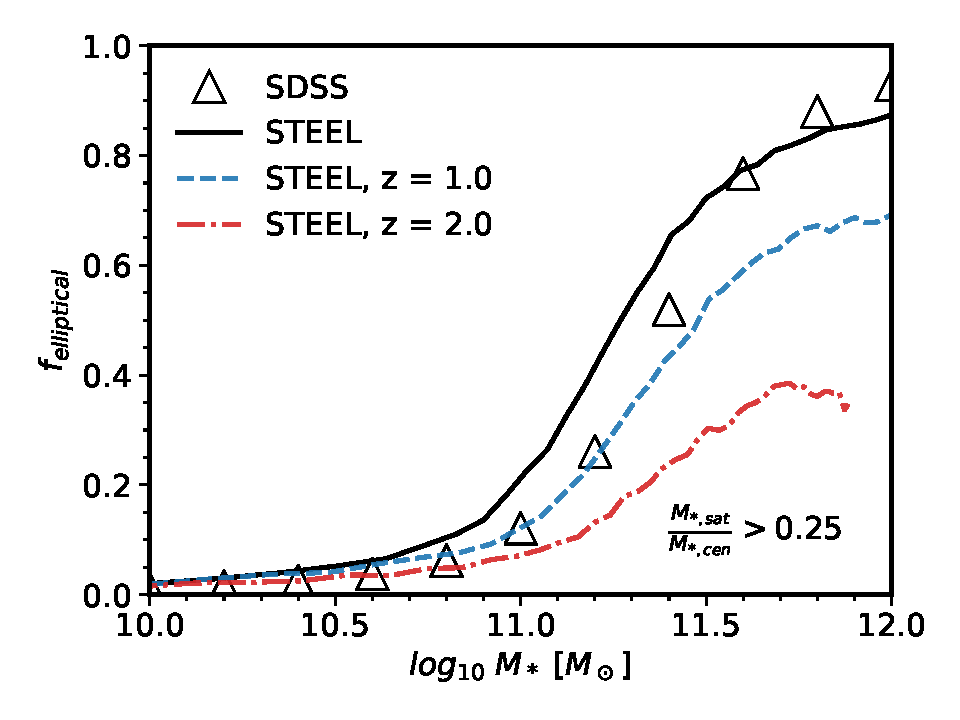
\includegraphics[width = \linewidth]{Figures/Chapter5/GalaxyMorphologies.pdf}
	\caption{We show at three redshift steps the predicted fraction of ellipticals as a function of stellar mass. The lines are the predictions from \textsc{steel} and the triangles are the T-Type selected elliptical fraction from SDSS at redshift $z = 0.1$.}
	\label{fig:Gal_Morph}
\end{figure}


\section{Lenticular Galaxy Formation}
%What is a lenticular and why are they considered independently to the rest of the galaxy population?
Lenticular galaxies are categorised by their unusual appearance, in the famous `tuning fork' diagram derived from \citet{Hubble1927TheNebulae} the lenticular galaxies are found where the two spiral `forks' meet the elliptical `handle'. Lenticulars similar to spirals have an extended disk but do not boast the `bars' or `arms' that decorate the disks of spiral galaxies nor the resiviors of cold gas suitable for star formation \cite{CHAMARAUX1986TheSamples}; similar to ellipticals lenticulars have a velocity dispersion dominated bugle at their centre. 
%What have been the proposed models of Lenticular formation?
Given that lenticulars sit between and share properties of both the other types of galaxy it is reasonable to think that they could exist on the transformation pathway between the two populations. This finding is potentially supported given lenticulars are preferentially found in the cluster environment \cite{Dressler1980GalaxyGalaxies} and the fraction of lenticulars increases with decreasing redshift simmilar to that of ellipticals \cite{Postman2005TheClusters}. 
%Building a least assumption model of lenticular formation (supervised project)
\subsection{Lenticular formation in empirically constrained environments.}
\textit{The work presented in this subsection was carried out by SP under the supervision of PJG and FS. The direction of the project was heavily influenced by PJG and builds upon the successes found in predicting morphologies in \steel.}
Given the successes in ratifying the simple merger model of elliptical formation within \steel, we use several literature suggested models of lenticular formation to build a `minimal assumption' model that fits the morphological fractions from SDSS.

\subsubsection{\citet{Cook2009Two-phaseFormation} Model}

We started our investigation by implementing the lenticular formation model from \citet{Cook2009Two-phaseFormation}. This model divides halo growth into two distinct phases, a fast collapse and intense merging phase at high redshift and a slow accretion low redshift phase after a transition epoch $z_{t}$. The galaxy growth related to this two phase halo growth is that the spheriod forms at high redshift and the disk at low redshift. The model for building spheorids in this semi-analytic model is the same as that implemented in \citet{Granato2004AHosts}. 

Translating semi-analytical techniques into a semi-empirical model by nature of the two models results in a loss of complexity, to distil this model we focus on the two phase formation. Galaxies are selected where they have grown a significant fraction of their mass (e.g. 70\%) between two epochs as assigned as lenticulars. These galaxies can then undergo further evolution by being transformed into ellipticals as described by the merger model from the previous section. Despite utilising complete freedom in the mass fraction required and redshift thresholds we find that within the framework given by \steel this model can not reproduce the lenticular fractions as shown in Figure \ref{fig:CookeModel}.

\begin{figure}
  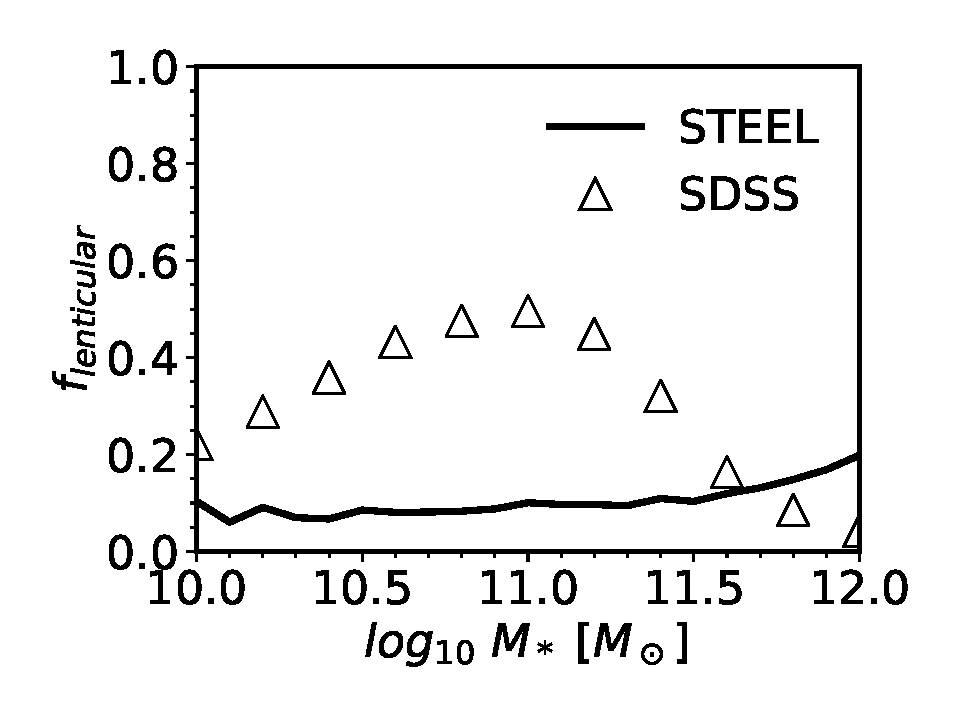
\includegraphics[width=\linewidth]{Figures/Chapter5/CookModel.pdf}
    \caption{Lenticular galaxy fractions generated using a very simplified
      version of the lenticular formation method described in
      \cite{Cook2009Two-phaseFormation}. The model assumes lenticular galaxies are those that have formed during a particular epoch. That is, we can label galaxies that grew to more than, e.g. 70\% of their mass within some defined epoch as being
      lenticulars. However, even after significant optimisation of the mass
      threshold and epoch definitions, it is not possible to reproduce the SDSS
      data within \steel using this model.}
    \label{fig:CookeModel}
\end{figure}

\subsubsection{Minimal assumption model}

Given the unsuccessful implementation of the \citet{Cook2009Two-phaseFormation} model we revisit other literature proposed models to find out which (or combination of which) have the potential to generate the observed lenticular fraction. Considering the nature of lenticulars in observations which increase their fraction with decreasing redshift in a similar fashion to ellipticals the first model we implement extends that of the elliptical merger model. An additional merger mass threshold ($\mu$) is implemented at $\mu = M_{*, sat}/M_{*, cen} = 0.05$ central galaxies that experience a merger in this mass range are assigned to be lenticulars. Lenticular galaxies that then experience mergers above the ratio are reassigned as ellpticals. This essentially adds a central 3rd column to Figure \ref{fig:Gal_Morph_toon}. As can be seen in the first panel of \ref{fig:Lentcular_panels} this simplistic model over produces lenticulars in the high mass end. Following simmilar ideas to the gas dissipation models utilised in \citet{Hopkins2009} we test a hard gas threshold. Physically this gas threshold can be interpreted as a damping force, the gas dissipates the energy of the merger into heating the gas reservoir limiting the disruption to the galaxy structures. Initially only galaxies with a gas fraction above the threshold can be converted into lenticulars, as shown in the middle panel this removes all lenticulars from the high mass end where galaxies tend to be gas poor. 
Finally, to improve the fit a soft gas fraction is implemented where galaxies below a given mass fraction become statistically less likely to become lenticulars after experiencing a major merger. We include the soft gas threshold to reflect the efficiency of the gas ratios at dissipating the energy. This combination of models well fits the high mass lenticulars as can be seen in the rightmost panel of Figure \ref{fig:Lentcular_panels}.

\begin{figure}
  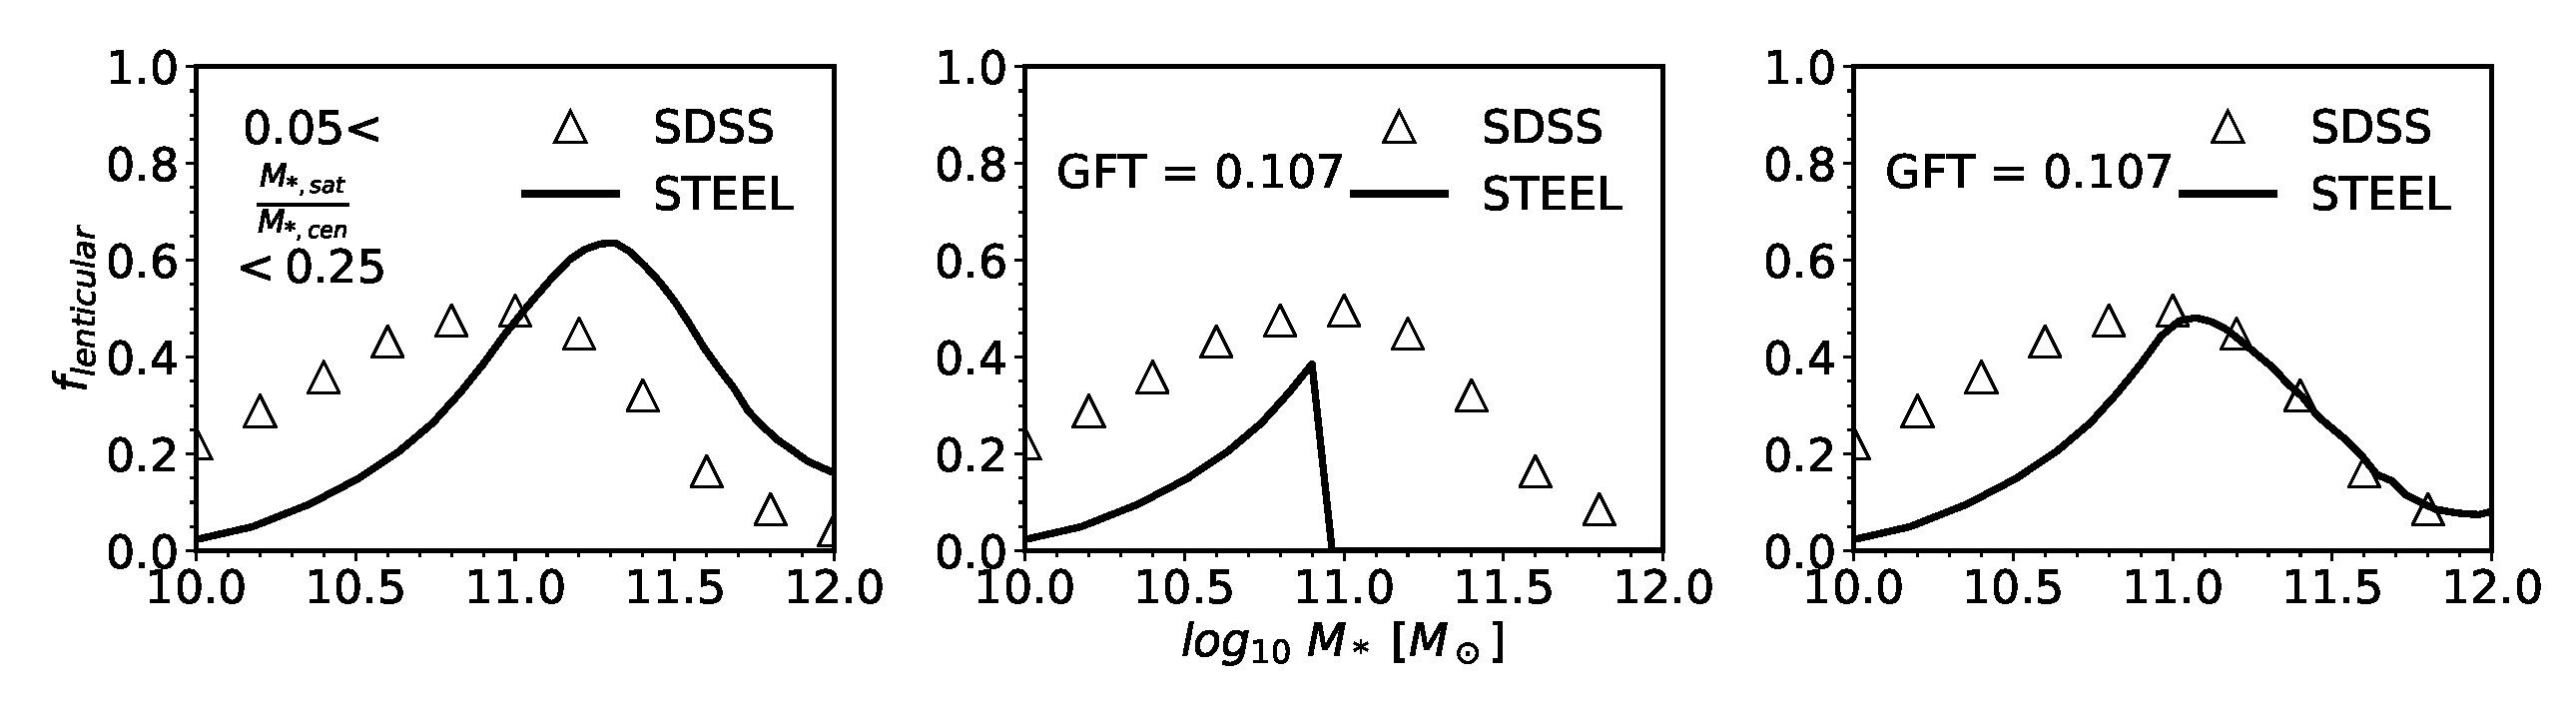
\includegraphics[width=\linewidth]{Figures/Chapter5/Lenticular_three.pdf}
    \caption{Three plots from left to right show lenticular fractions generated using the progressive development of the lenticular merger model. The first (leftmost) panel shows the fraction generated by summing the number densities of merging galaxies with mass ratio in the range $0.05 < \mu < 0.25$. The middle panel shows the effect of adding a hard gas ratio cutoff to the merger model, galaxies that are above a gas fraction threshold (GFT) do not form lenticulars. Finally, changing the model to a `soft' gas fraction threshold where the efficiency of lenticular formation is reduced above the GFT.}
    \label{fig:Lentcular_panels}
\end{figure}

Lower mass galaxies reside in less rich environments and grow more via secular (in-situ) processes, it is therefore understandable that the merger/dissipation model does not make lenticulars at these masses.

To build lenticulars at these masses we implement a disk instability model following the baryonic inflow rates given by \citet{Bournaud2011BLACKSTREAMS}. Applied along the accretion histories we allow galaxies to build their central bulges though gas transport from the disk using Equation \ref{eqn:DiskInflow}, 

\begin{equation}
    \label{eqn:DiskInflow}
    \dot{M}_{inflow} = 25 log_{10}\Big[\frac{M_{*,disk}}{10^{11}}\Big]\Big(\frac{1 + z}{3}\Big)^{1.5},
\end{equation}

the mass of the bulge is then given by,

\begin{equation}
    M_{bulge} = \sum_z \dot{M}_{inflow} \times \delta t(z),
\end{equation}

in each mass bin a fraction of galaxys proportional to the mass ratio of the bulge to the total stellar mass, $A \times M_{bulge} / M_{*, total}$, is added to the lenticular population. The resulting fit to the population is shown in Figure \ref{fig:All_Morphologies}.

\begin{figure}
  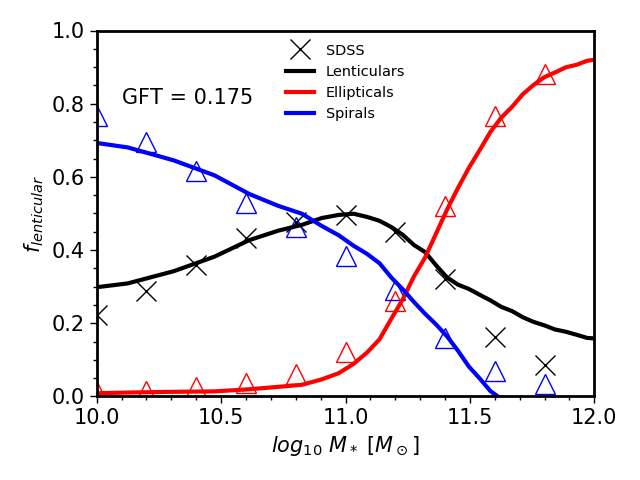
\includegraphics[width=\linewidth]{Figures/Chapter5/Bulge_Growth_Final_All_Morph.png}
    \caption{We show the fractions of morphologies as a function of mass. Ellipticals are generated using a major merger model, lenticulars using the combined merger (with soft gas fraction) and baryonic inflow models} and, spirals are the remaining population.
    \label{fig:All_Morphologies}
\end{figure}

We find the combination of a merger and inflow model is able to adequately recreate the lenticular fractions. This two model fit is potentially consistent with the distinct morphological types, barred and un-barred found within the lenticular population \cite{Laurikainen2005MulticomponentGalaxies, VanDenBergh2012LuminositiesGalaxies}.

In summary, to recreate the lenticular population we find it necessary to add three parameters in addition to the major merger mass ratio used to create the ellipticals. The first is the `minor' mass ratio limit that defines the minimium mass ratio at which lenticulars are formed via mergers, the second the is the `soft' gas mass threshold that damps the creation of lenticulars and, finally the parameter to convert the bulge ratios to lenticular fraction. 

\section{Discussion}

In this chapter we have shown two applications of \steel. Firstly is the ability of \steel to unravel the effects of systematics in galaxy observables using the galactic pair fractions. Secondly, we show an example of how constrained merger histories can be used to test if proposed morphological evolution models recreate the observed morphological fractions.  

\subsection{Pair Fractions}

The primary goal of the pair fraction analysis is to show the propagation of systematics in galaxy modelling. 
Specifically, we use the SMHM relationship to connect assumptions used when estimating stellar masses from observations to systematics in galaxy pair fractions in the context of a \LCDM Universe. 
In this chapter we have used two observed stellar mass functions from SDSS-DR7 observations that use a de Vaucoulers and a S\`ersic + Exponential fit to determine stellar masses, which in turn generate stellar mass functions with notably different number densities at the high mass end. Each stellar mass function then generates, through abundance matching, a different SMHM relationship. The S\`ersic + Exponential mass function generates a steeper high-mass slope in the SMHM relationship at any epoch.
In addition to the SMHM relationships from the observed data we use a relationship fitted to match the outputs of the Illistris simulation. Furthermore, we also consider a toy model SMHM relation individually perturbing each input parameter to transparently probe the impact of the input SMHM relation on the pair fractions.
In each case we find that small changes introduced into the SMHM relationship can have significant effects on the expected pair fractions, as shown in Figures \ref{fig:MassRatioCartoon},\ref{fig:SMHM_PF_Cartoon}, \& \ref{fig:PairFracSystematic}.
This suggests that in the contxet of a \LCDM Universe tensions in previous observational studies could, in large part, be traced back to systematics in stellar mass estimates.

In \citet{Mundy2017A3.5} the $M_{*,cen} > 10^{10} M_{\odot}$ pair fraction is given, however, this is not significantly different from the $M_{*,cen} > 10^{11} M_{\odot}$ pair fraction shown in Figure \ref{fig:PairFractionData}. In Figure \ref{fig:PairFracSystematic} we find the pair fraction drops significantly when mass a selection is taken below the SMHM relation knee. As this drop is not found by \citet{Mundy2017A3.5} we interpret that their pair fraction measurement is not consistent with a break in the SMHM relation between $10^{10} M_{*,cen}$ and $10^{11} M_{*,cen}$.

\citet{Man2016RESOLVING03} noticed that the choice between luminosity-selected and stellar-mass selected pairs affected the pair fraction evolution. In this work we have provided a clear framework to properly interpret how input choices create systematic effects in the observed pair fraction and its evolution. Furthermore, it is a common approach to infer the assembly history of galaxies by converting the pair fractions into merger rates by assigning timescales to galaxy pairs \citep{Conselice2003A3,Conselice2008TheField,Mundy2017A3.5}. 
In \Paper{2} we developed a model that calculates the stellar mass growth rates of central galaxies and the stellar mass accretion rate from satellite galaxies.
It is found that, for some SMHM relationships, the accretion rate can be greater than the total growth rate implying the model is internally inconsistent and the SMHM relationship is not compatible with this \LCDM cosmology.
The stellar mass accretion rate is connected to the merger frequency and therefore the galaxy pair fraction. 
In this work we connect the shape and evolution of the SMHM relationship to the evolution of the pair fractions.
We propose it is therefore possible to use the pair fraction as an additional constraint to the SMHM relationship, this is a natural extension of conditional abundance matching or extended SHAM (subhalo abundance matching) models \citep{Hearin2013SHAMGroups}.
Using \steel one can test simultaneously the accretion ratio and the pair fraction generated from a given stellar mass function and cosmology.

Any changes to the stellar mass estimates such as photometry, background subtraction, IMF, e.t.c. that affect the stellar mass function will in a given cosmology create a change in the SMHM relationship. Therefore by the systematic propagation demonstrated in this work any stellar mass estimation will create systematic differences in the pair fractions. 
With the techniques presented throughout this thesis, one could retrieve the systematic differences created in pair fraction under multiple \LCDM cosmologies and for any given set of stellar mass functions. As a further test of our results we show the pair fractions found in Illustris, together with the pair fractions predicted by \steel, using a SMHM relationship designed to match
that of Illustris are fully consistent.

In the era of wide and deep surveys, such as EUCLID, constraining a model using a single multi-epoch data set with consistent photometry will become a reality. The advantages of this are twofold: By tuning the SMHM relation to a given survey over a large range of redshifts the growth of the stellar mass function over time can be tested against the implied satellite accretion and star formation rate as in Chapter \ref{Chapter:GalGrowth} this can be seen as a test of the consistency of the cosmological model or of the consistency of the stellar mass and/or starformation rate estimation. Secondly, as in Chapter \ref{Chapter:GalDist} one can test if the high redshift SMHM relation is consistent with the low redshift satellite distributions. The constraints on a given photometry, cosmological model, satellite evolution, starformation rate, e.t.c... are still not complete however it will allow nonphysical results to be identified. Furthermore, by making the model accessible it can then be used in the manner described above to make systematic adjustments to compare between current and future data sets that may use different stellar mass estimations.

\subsection{Morphologies}

Given the very promising results of \steel in predicting satellite number densities in different environments and epochs, we here take a step further and explore whether \steel's cumulative number of major mergers is able to account for the local fraction of elliptical galaxies as well as implementing several literature inspired lenticular formation models. 

Despite the noticeably good agreement between model predictions and data in Figure \ref{fig:All_Morphologies}, we stress that different input SMHM relations can, as shown in this Chapter \ref{Chapter:GalGrowth}, substantially affect the accretion rate which in turn will modify the number of galaxies experiencing major mergers. It follows that any cosmological galaxy evolution model that uses mergers as a physical driver for galaxy transformation should first simultaneously and self-consistently closely reproduce stellar mass functions, the SMHM relation, satellite distributions, and pair fractions at previous redshifts.

\section{Conclusions}
\label{sec:Conclusions}

In this Chapter, we show that the input SMHM relations, based on different stellar mass estimations, have a significant impact on the predicted galaxy pair fraction. In short, the steeper the relation, the lower the pair fraction. Specifically we compare stellar mass functions created with a de Vaucoulers-based photometry (cmodel) to a S\'ersic-Exponential photometry (PyMorph), the latter leading to an enhancement in the number density of high mass galaxies. The resulting effect of these stellar mass functions is a different input SMHM relation to $\steel$, the primary difference consisting of a steeper high mass slope when adopting the S\'ersic-Exponential profile. As expected, the S\'ersic-Exponential results in a lower pair-fraction. To attempt to explain the difference in pair-fraction evolution with redshift we create a suite of toy models testing different alterations to the SMHM relation. We find that this evolution is linked to the evolution of the high mass slope.

The purpose of this work is to show how subtle changes in derivation of stellar mass could lead to large differences in the pair fraction observed. It is therefore crucial when comparing two different samples to account for the systematic biases introduced by the assumptions implicit in stellar mass estimation as shown in this work to avoid systematic effects from a simulations foundation propagating to more `delicate' physics or driving unwanted feedback processes.

The second part of the chapter showed how simple morphological models can be quickly implemented in \steel to show how they propagate into the galaxy populations. We are able to show that some models such as the major merger model well reproduce the observed distributions as is expected from it widespread use in semi-analytic modelling. The example of building a `least assumption' model shows how the transparency of the empirical and statistical approach can aid the testing and development galactic modelling. ARGHHHHH

Future surveys should look to use fast and flexible modelling alongside data products to be able to properly understand the systematic effects of assumptions made on derived data products. For example the SMHM relation must simultaneously fit: traditional abundance matching, self-consistency between satellite accretion and central galaxy growth, and as shown in this paper the normalisation and evolution of the galaxy pair fraction. This multi-product fitting will ensure relations such as the SMHM relation are better constrained. The methods described in this work and \Paper{2} will also provide more stringent theoretical limits to the stellar mass estimations and photometerys used for future surveys.
 % Discuss Galaxy pair fractions and the systematics thereof how this impacts mergers and morphologies 

% Chapter 6

\chapter{Conclusion} % Write in your own chapter title
\label{Chapter:Conclusion}
\lhead{Chapter 6. \emph{Conclusion}} % Write in your own chapter title to set the page header
\begin{center}
    \textit{``We gaze continually at the world and it grows dull in our perceptions. Yet seen from another's vantage point, as if new, it may still take the breath away.''}
    Alan Moore - Watchmen
\end{center}


This thesis describes $\steel$, the STastical sEmi-Empirical modeL, a model designed to use the empirical technique in a new fashion. The design of \steel allows for extremely fast, flexible and transparent testing of a variety of galaxy formation theories. The novelty introduced by the statistical dark matter accretion histories allows \steel to make predictions that would be limited with other traditional (discrete/non-statistical) numerical or analytic tools of galaxy formation. The foremost problem concerning galactic modelling on a cosmological scale is represented by the large number of physical processes at play at different scales and the limited knowledge in how to describe them. Complexity and uncertainty are built into models from all contributing aspects, from the dark matter simulations \cite[e.g.][]{vandenBosch2018DisruptionFiction}, to observations \cite[e.g.][]{Bernardi2017ComparingLight, Lapi2017StellarEquation, Leja2019AnSurvey}. Techniques have been developed to try to reduce the impact of these complexities, for example:
\begin{itemize}
    \item To reduce the need to build stellar mass from first principles following the gas collapse. Abundance matching is used to create a mapping between galaxy stellar mass at the centre of a halo and the mass of the host halo itself at any redshift accessible by observations. In doing so it provides a robust framework to model the evolutionary tracks of galaxies following the growth of their host dark matter haloes.
    \item To remove tensions between conflicting observations such as the cosmic stellar mass density and cosmic star formation rate. Continuity modelling is used to predict the star formation rate using the evolution of the stellar mass function from high to low redshift. 
\end{itemize}

The impact of publication bias, the preferential publishing of positive and novel results, is a known problem in academic disciplines \cite[e.g.][]{Song2010DisseminationBiases}. It is unsurprising then that the number of papers that report new techniques or fits to data far outweighs those models which deconstruct the techniques to understand how our models work and document their limitations \cite[e.g.][]{vandenBosch2017DissectingSimulation, vandenBosch2018DisruptionFiction, Asquith2018CosmicModels}. Additionally, it can be expected that, for example, tuning of high parameter systems to create high fidelity matches to data, will generate a higher publication impact than equally important analysis tools. The design of \steel has been influenced by this culture. We prioritise the understanding of systematics and internal self-consistency above that of fitting new features. Where new features are introduced they use modular and flexible modelling techniques that can be analysed independently.


\steel is a statistical model and not a physical model, in this way is the antithesis of high-resolution single galaxy or cluster simulations such as FIRE \cite{Hopkins2018FIRE-2Formation}. Galaxy modelling is currently based on a large spectrum of techniques from hydrodynamical simulations, through semi-analytic and semi-empirical models, to mock catalogues produced via HOD. In this regime, \steel can be thought of as occupying a space between traditional semi-empirical and HOD modelling. We retain the ability to track galaxy populations in redshift but forgo the tracking of discrete objects from step to step. Despite the antithetical nature of \steel to the hydrodynamical and non-statistical models, it is not adversarial, used in conjunction with other techniques it will prove to be a valuable tool for the galaxy modelling community. 

\section{Pros and Cons of \steel as a Galaxy Model}
%successes of STEEL where other models fall down
%what if theoretically impossible in steel that other models can do

\steel has had the following major successes:
\begin{itemize}
    \item Reproduction of the statistical distribution of satellite galaxies in dark matter halos over a broad range of redshifts and halo masses, a challenge for traditional \LCDM models. (Chapter \ref{Chapter:GalDist})
    \item Identification of the inconsistencies between certain stellar mass functions and dark matter accretion histories produced by \LCDM cosmologies. (Chapter \ref{Chapter:GalGrowth})
    \item Derivation of the star formation rate from a new halo centric approach, consistent with cutting-edge observations.(Chapter \ref{Chapter:GalGrowth})
    \item Analysis of the systematic effects the estimation of stellar-masses has on the observed galaxy pair fraction. (Chapter \ref{Chapter:GalPairs})
\end{itemize}
Each of the points listed above directly stems from the statistical approach of \steel to dark matter accretion histories. However, this technique loses individual galaxies that could be tracked through hydrodynamical, semi-analytic, and traditional semi-empirical models.

\steel is an exceptional tool for systematic modelling, by applying predictions to statistically significant volumes we are able to draw transparent conclusions about the way assumptions and models propagate into observed populations. Furthermore, Chapter \ref{Chapter:GalPairs} shows the potential of this systematic technique to track how changes to input propagate to output in a complex system, as shown with the pair fractions. Additionally, STEEL allows for fast,  effective, and precise testing of a variety of recipes for galaxy evolution, such as the formation of bulges via mergers and disc instabilities.

\section{Impact of \steel}
%how impactful is the work done with STEEL on the wider field?

\subsection{Modelling}

Creating another cosmological model acting on a discrete dark matter background has little value to add to the large number of competitive models already existing in empirical, \cite[e.g.][]{Rodriguez-Puebla2017ConstrainingProperties, Moster2018Emerge10, Behroozi2019UniverseMachine:010, Zavala2012}, analytic \cite[e.g.][]{Somerville2015StarGas, Guo2011FromCosmology, Fontanot2007ReproducingCosmogony, Zoldan2019TheEvolution}, and hydrodynamical \cite[e.g.][]{Springel2018FirstClustering, Hopkins2018FIRE-2Formation, McAlpine2015TheCatalogues} regimes. The systematic statistical approach of \steel can be used to complement these models in two ways:
\begin{itemize}
    \item Pre-Processing: 
    \begin{itemize}
        \item \steel can be used to test the validity of the combinations of input data. For example as in Chapter \ref{Chapter:GalGrowth} we combine the dark matter assembly histories with two different stellar mass functions to test if the satellite galaxy accretion is consistent with the central galaxy growth. We find only one of the two tested SMF to produce an internally self-consistent satellite accretion - central mass growth. By validating the input data before running the simulation we ensure the output validity in advance of resource/time commitment.
        \item \steel can rapidly test the ability of different theoretical models to reproduce key observables such as the morphological mix of galaxies in the local Universe or the star formation rate distributions. 
    \end{itemize}
    \item Cosmological extrapolation: 
    \begin{itemize}
        \item STEEL can generate accurate predictions for a given galaxy model over scales covering many orders of magnitude, unfeasible for current hydrodynamic simulations. For example, \steel can produce the distributions of massive satellites over a large scale range from groups to very massive clusters, to high redshifts in good agreement with data. Whilst the predictions for the group-scale are in good agreement with the Illustris TNG simulation, the cluster-scale is a new achievement of STEEL, not present in the Illustris TNG simulation.
    \end{itemize}
\end{itemize}
\subsubsection{Data}

We have shown how \steel can be used to combine data with a given cosmology to: predict stellar-mass - dark matter assembly consistency, satellite distributions, and star formation rates. This has been used to add weight to the claims made about light profiles from \citet{Bernardi2017ComparingLight} and the star formation rates from \citet{Leja2019AnSurvey}. In each of the aforementioned works, problems are identified in current data analysis and more advanced data fitting routines are used. Specifically, \citet{Bernardi2017ComparingLight}  introduced their PyMorph photometry algorithm which provides more robust fitting to the light distributions of especially the more massive galaxies and more careful subtraction of the sky background. \citet{Leja2019AnSurvey} put forward a state-of-the-art Bayesian SED fitting model, Prospector-alpha, that better accounts for the emission from old stars, thus lowering the amount of younger stellar population and overall SFRs. The previous examples show that \steel has a valuable contribution to make to the validation of data fits, fully realised it could become an integral part of data fitting routines bringing theory closer to observations.

\section{Future of \steel in Galactic Astrophysics}
\label{sec:Future}
%How can we build on what we have done?

The future of \steel and potentially the future of statistical semi-empirical modelling now relies on communication of the advantages (and disadvantages) of the technique. We have begun to build collaboration around the model with several other empirical modellers, dark matter physicists, observers (both survey designers and data analysts), as well modellers that use semi-analytic and hydrodynamic models. The reception to \steel has been widely positive with many intrigued by its unique capabilities. The most notable group involved is the EUCLID consortium. Working with EUCLID, \steel has the potential to provide firm constraints on the expected number of pair fractions, mergers, and ellipticals at different redshifts (one of the main aims of Work Package 5, for example). To provide the best performance, \steel will need to input the same stellar mass reference system as adopted in the survey.

PJG outlined the methodology to create \steel alongside a 4-year development plan for a fellowship proposal\footnote{Unfortunately unsuccessful, the proposal and related documents are included in full in Appendix \ref{Appx:HF}.}. In this plan the future of \steel was separated into two complementary pathways, a data fitting tool and a galaxy modelling tool, presented below:

\subsubsection{Data fitting tool}

HOD modelling is a popular analytic tool used to create galaxy mocks in terms of the average number of central and satellite galaxies above a certain luminosity/stellar mass threshold as a function of host halo mass. Using relationships such as HOD number counts, or a simple SMHM relation from abundance matching, can produce galaxy mocks onto a dark matter simulated light cone, which in turn can be used for predictions on observed number counts above the flux limit of a survey. This kind of modelling is done prior to first light and far separated from the actual photons to be received. With \steel we can outperform traditional mock modelling. \steel can not only predict galaxy number counts for any given SMHM relation derived from measured SMFs, but it can also check for self-consistency in the measured SMFs and thus guide the overall initial fitting procedure. More specifically, \steel can check if the total galaxy growths implied by the assumed SMF/SMHM relations are larger than the total stellar mass assembled via satellite accretion, a condition that, as we discussed in Chapter \ref{Chapter:GalGrowth}, can be violated in a \LCDM Universe.

Using Figure \ref{fig:Full_Mod_Toon} we show how \steel can be positioned to become a key element of observational fitting bringing theory and observation much closer than ever before. \textcolor{MPLgreen}{The observational inputs (green) are twofold, the survey, i.e., the flux received on the telescope which is the only constant in the system, and the observational fits, which are used to derive physical attributes from the collected photons. In this example the survey and fits generate the stellar mass function (SMF).} \textcolor{MPLred}{Secondly, the dark matter cosmology is input in $\steel$\footnote{it is worthy of note that the exact cosmological parameters may also influence the fits used.}. As described throughout this thesis, \steel uses halo mass functions (HMF), halo substructures, and halo growth histories which are then combined to generate a statistical dark matter accretion history.} Most of the baryonic (SMF) and DM (accretion histories) inputs described above are flexible and fast to model. \textcolor{MPLblue}{However, the final modelling usually adopted to interpret the data is traditionally computationally intensive, time-consuming, and often degenerate. The empirical approach, especially as used within $\steel$, offers solutions to these problems being computationally light, fast, and transparent.} As described in Chapter \ref{Chapter:GalGrowth}, using Figure \ref{fig:SFRDerevation_Cartoon} we can derived the star formation rate and bimodality using a combination of \textcolor{MPLgreen}{observation}, \textcolor{MPLred}{cosmology}, and \textcolor{MPLblue}{modelling}. Through comparison of modelled properties to observations, we can test that all elements of theory and data used are self-consistent and evolve appropriately together within a given cosmology e.g.
\begin{itemize}
    \item Satellite galaxy distribution
    \item Pair fraction
    \item Star formation rate / cosmological star formation density
    \item Star formation - stellar mass function continuity
    \item Galaxy bimodality
    \item Galaxy morphology
\end{itemize}
\begin{figure}[t]
    \centering
    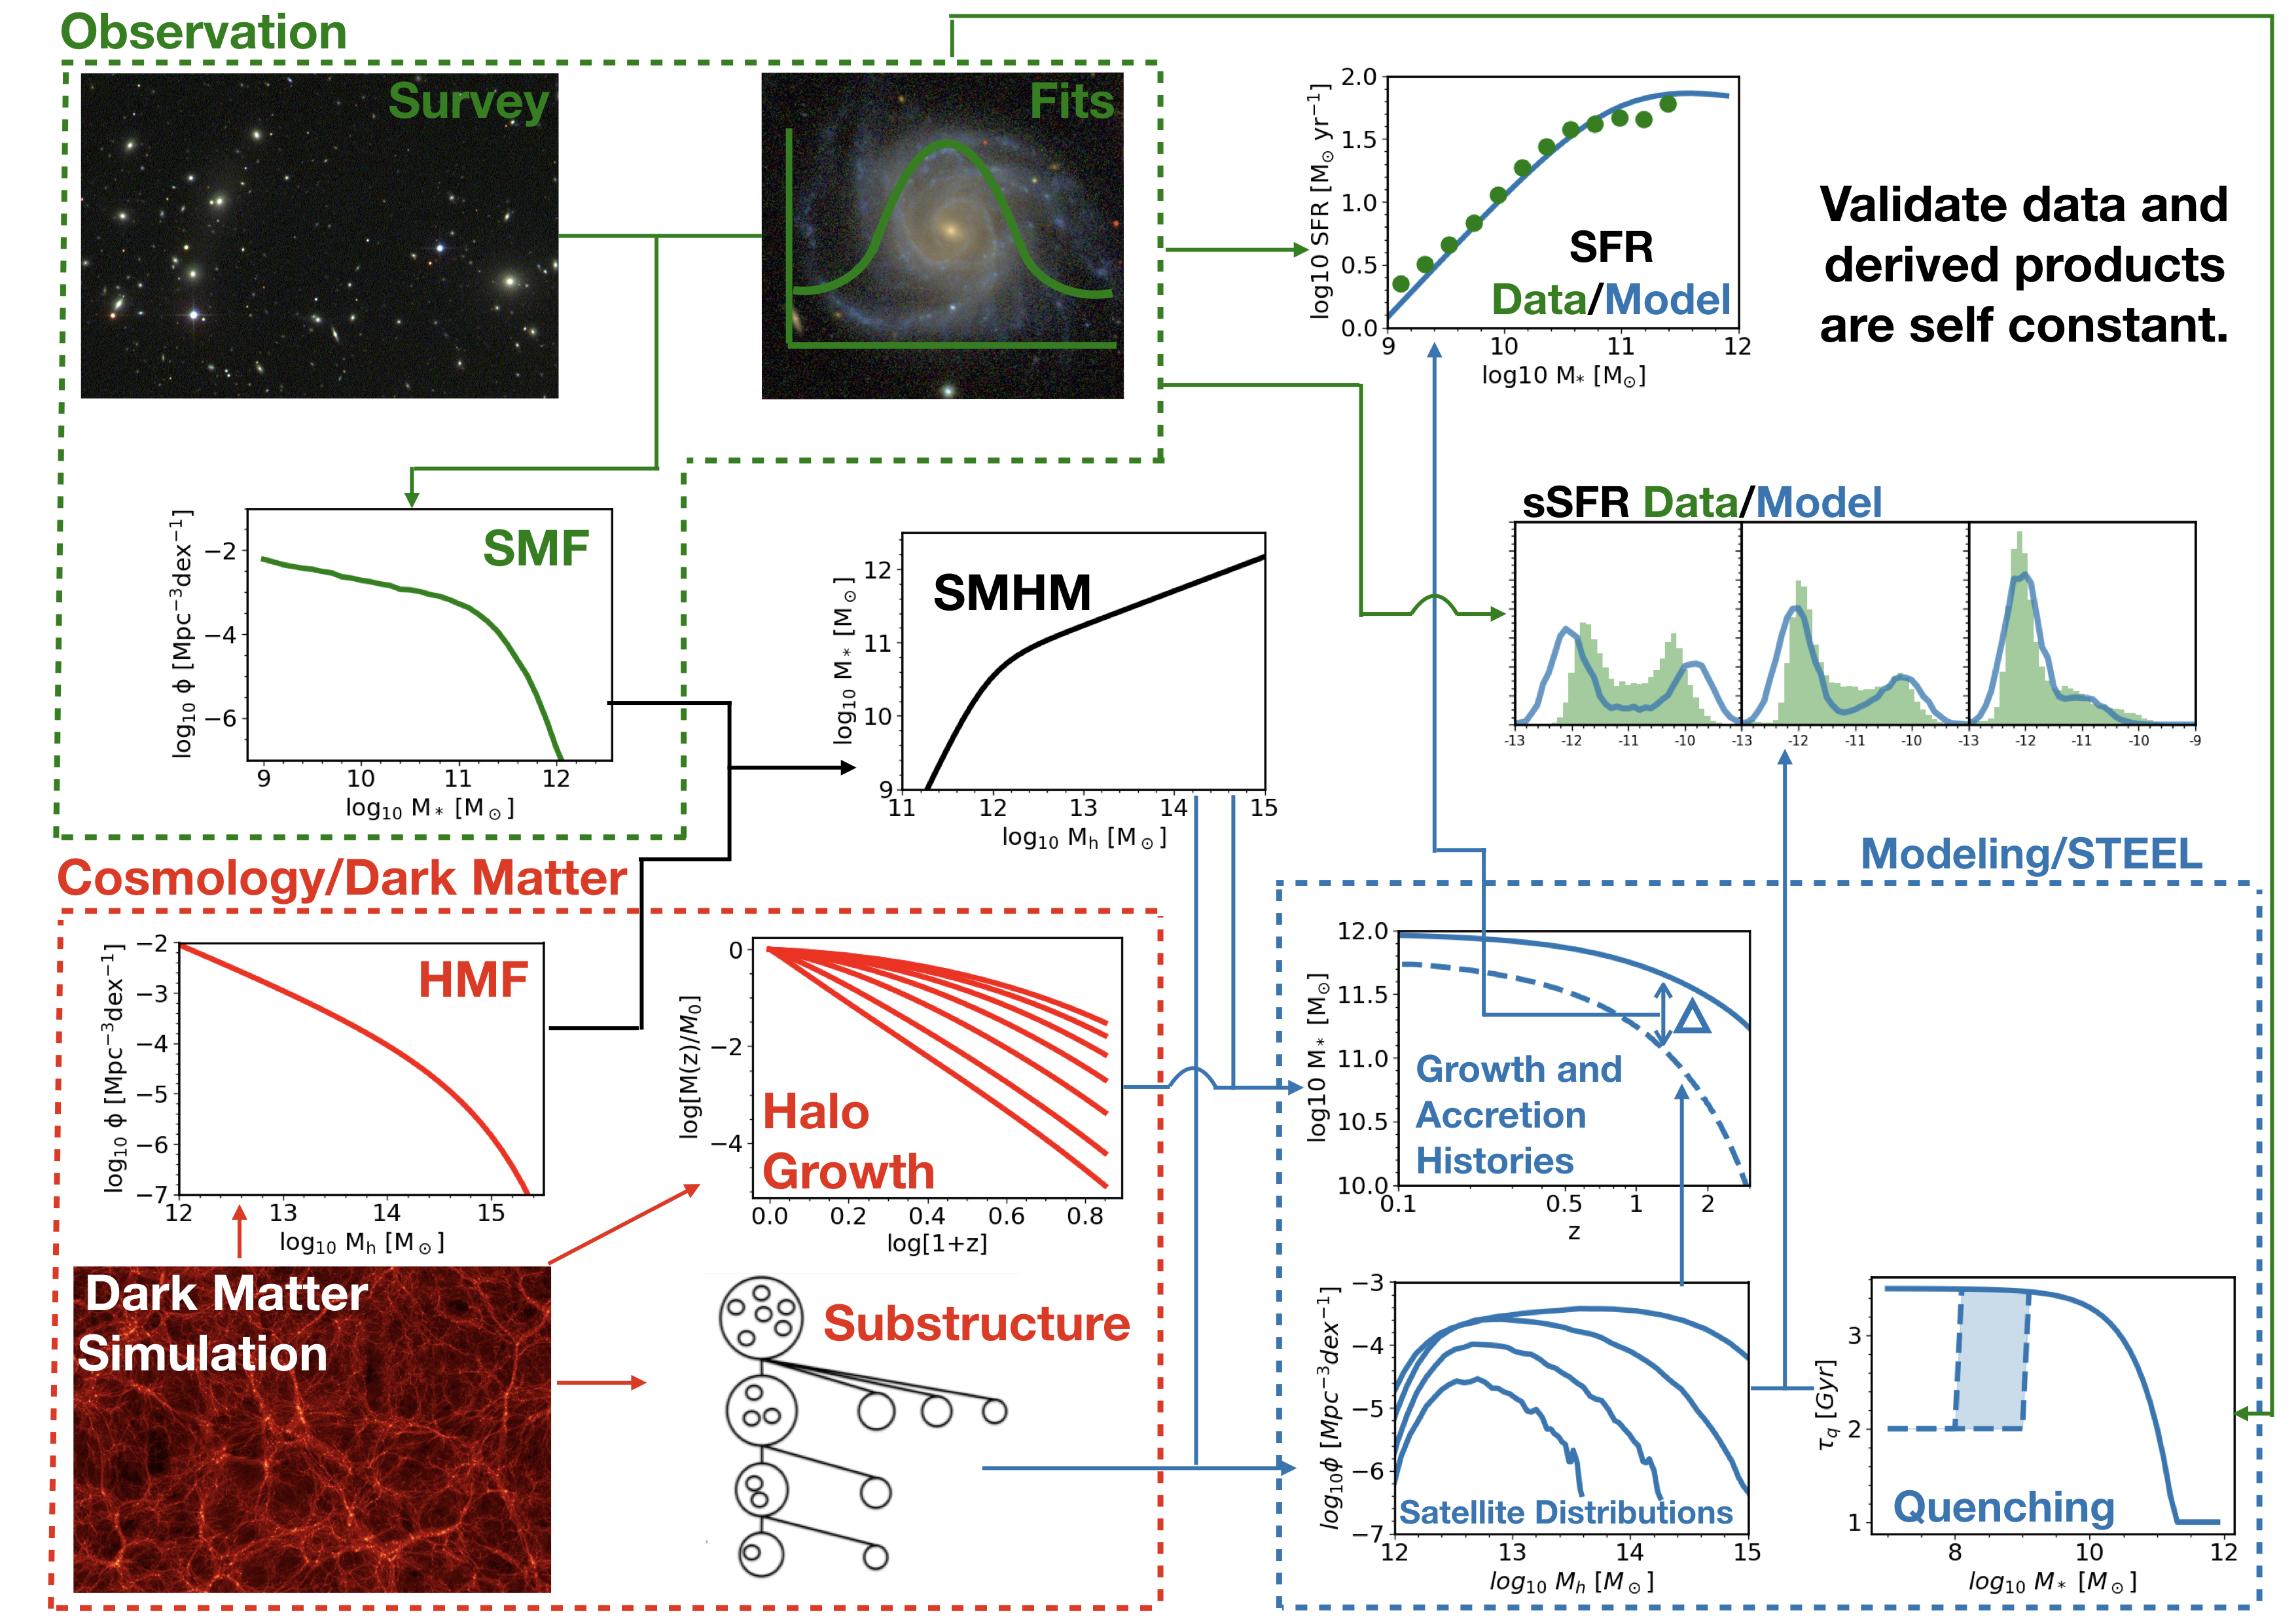
\includegraphics[width = \linewidth]{Figures/Chapter6/FullModelCartoon.png}
    \caption{Schematic cartoon related to Figure \ref{fig:SFRDerevation_Cartoon} of how \steel can be used to check for self-consistency between fitting models used on observed data and the theoretical assumptions that underpin the fitting models.}
    \label{fig:Full_Mod_Toon}
\end{figure}
Items closer to the top of the list are less affected by the modelling and therefore likely to be more robust within this method. Given empirical techniques use observation as inputs to modelling, having an empirical model as part of a data fitting pipeline the model will have the potential to reject/modify its own inputs by influencing the parametrisation of the observational data reduction routines. This fitting, checking, refitting, cycles will ensure that any mismatch between the observational fit and the modelled property can be addressed from multiple distinct angles appreciating the uncertainties inherent in fitting, modelling, and cosmology together.

\subsection{Galaxy modelling tool}

$\steel$, built around the concept of a statistical dark matter accretion history, can be regarded as a new competitive tool in the modelling of galaxies. This is due to two factors: firstly, the ability to simulate without limits on volume or resolution, thus allowing to model even the rarest objects in the Universe, a feature that is not realistically achievable by other modelling techniques; secondly, the removal of discrete objects allows for a new type of continuity check where the consistency of populations is modelled as a priority instead of the consistency of individual haloes/galaxies. 

\steel is an excellent start to statistical semi-empirical modelling. With any future revision, the model should be updated in the following ways:

\begin{itemize}
    \item The statistical dark matter accretion history should be a separate library, containing flexible cosmology, halo definitions (e.g. virial, splash-back, m200c, e.t.c...), and should be built in an object-oriented fashion such that it is easily extendable.
    \item The galaxy modelling should be redesigned such that each dark matter accretion history is built upon using explicit probability distribution convolutions.
    \item The outputs should be shaped by the statistical dark matter accretion history and contain structured probability distributions to be able to post-process a hierarchical complexity of results.
    \item The post-processing suit should contain any and all integrators required to process the outputs into galaxy populations for cosmological volumes, single mass tracks, or given mass ranges.
    \item The post-processing suit should offer `views' on the data structure using flexible plotting routines for ease of query and graph creation by a non-expert user similar to the API provided to IllustrisTNG \cite[][https://www.tng-project.org/data/vis/]{Nelson2019TheRelease} as well as a more complex return structure to extract the full data products.
\end{itemize}

As detailed in the PERT chart in Appendix \ref{Appx:HF}, this would take six months to one year of full-time development depending on the programming and empirical modelling skills of the developer. Once developed, documented, and deployed such a tool would be of enormous value to the galactic astrophysics community. 

\section{In closing}

The applications of \steel detailed in Section \ref{sec:Future} each independently represent a tool that, if correctly developed and made publicly available, would be at the cutting edge of galactic astrophysics. The work done in this thesis represents the foundations upon which these tools can be built. 

In brief, the findings from this thesis can be summarised as follows: 
\begin{itemize}
    \item The dark matter structure and dynamics is the first-order driver for prediction of galaxy properties including, satellite distributions, star formation rate, galaxy morphologies. 
    \item Assumptions made during stellar-mass estimation produce significant non-trivial systematics in the pair fraction of galaxies and likely further properties, and without proper appreciation of such systematics, we are likely to fundamentally misinterpret the nature of galaxy assembly. 
    \item Stellar mass functions with an enhanced number densities of high mass galaxies are in much better agreement with \LCDM cosmology than those with lower number densities of high mass galaxies. Furthermore, some traditional stellar mass functions are fundamentally incompatible with \LCDM hierarchical cosmology.
\end{itemize}

To our knowledge, the complexities of the systematics behind galaxy pair fractions has never been addressed before in terms of the input SMHM relation. Finally, the lack of self-consistency between hierarchical \LCDM assembly and some stellar mass functions is a result of fundamental importance to galactic astrophysics that it was possible to achieve thanks to the statistical power of $\steel$. This result in particular hints at a potentially devastating departure between observation and theory that, if left unaddressed, will hinder our understanding of the evolution of galaxies for the foreseeable future.
 % Conclusion

%% ----------------------------------------------------------------
% Now begin the Appendices, including them as separate files

\addtocontents{toc}{\vspace{2em}} % Add a gap in the Contents, for aesthetics

\appendix % Cue to tell LaTeX that the following 'chapters' are Appendices

% Appendix EXTRASam

\chapter{Additional Semi-Analytic Methods}
\label{Appx:ExtraSAM}
\lhead{SAM methods Continued...}

In this Appendix, we detail a further common consideration taken in semi-analytic modelling, the state of the gas. The state can be calculated in several different ways, an empirical pressure based relationship is given by \citet{Blitz2006TheRelation}, the pressure in the disk is related to the ratio of molecular and atomic hydrogen. 

\begin{equation}
    R_{\mathrm{H}_{2}}=\left(\frac{\Sigma_{\mathrm{H}_{2}}}{\Sigma_{\mathrm{HI}}}\right)=\left(\frac{P_{m}}{P_{0}}\right)^{\alpha}
\end{equation}

The $H_1$ \& $H_2$ surface densities are given by $\Sigma_{\mathrm{HI}}$ \& $\Sigma_{\mathrm{H}_{2}}$, $P_m$ is the mid disk pressure, and $P_0$ \& $\alpha$ are additional free parameters. The gas partitioning can be calculated though an analytic model based on the connection between the interstellar radiation filed and the molecular self shielding \citep{Krumholz2008TheClouds,Krumholz2009THEDENSITIES,Krumholz2009THEGAS},

\begin{equation}
    f_{H_{2}}=1-\left[1+\left(\frac{3}{4} \frac{s}{1+\delta}\right)^{-5}\right]^{-1 / 5}
\end{equation}.

This is by no means a complete record of the various analytic recipes used in semi-analytic modelling. However here we have shown a subset of the multitude of free parameters that enable tuning of such models to achieve results consistent with observations.

\begin{equation}
s=\ln (1+0.6 \chi) /\left(0.04 \Sigma_{\operatorname{comp}, 0} Z^{\prime}\right),
\end{equation}
\begin{equation}
\delta=0.0712\left(0.1 s^{-1}+0.675\right)^{-2.8},
\end{equation}
\begin{equation}
\chi=0.77\left(1+3.1 Z^{\prime0.365}\right),
\end{equation}
where $\Sigma_{\operatorname{comp}}$ is the surface density for a given 100pc atomic-molecular cloud.

The final mechanism we discuss here is the enrichment of the galaxy and halo gas with metals. During the process of star formation and stellar mass, recycling metals are created. This is modelled as a batch process where $\mathrm{d} M_{Z}=y \mathrm{d} m_{*}$ where a mass $\mathrm{d} M_{Z}$ of metals is produced in each batch of star formation $\mathrm{d} m_{*}$, $y$ is a free parameter. The metal-enriched gas formed in this process is ejected by supernovae and assume instantaneously mixed with the cold disk gas. As supernovae are thought to be one of the main drivers of galactic wind the metals are thought to be preferentially ejected with the wind parameter $\zeta$ controls the ejected metal fraction, and the equation for the metal mass in the galaxy is updated as such,

\begin{equation}
\zeta=\zeta_{\mathrm{lo}} \exp \left(-M_{h} / M_{\mathrm{ret}}\right),
\end{equation}

\begin{equation}
\dot{M}_{Z}=y(1-R)(1-\zeta) \dot{m}_{*}+Z_{\text {hot }} \dot{m}_{\text {inf }}-Z_{\text {cold }} \dot{m}_{\text {out }},
\end{equation}

$\zeta_{10}$ and $M_{\mathrm{ret}}$ are free parameters, R is the recycled fraction and $Z_{\text {cold }}$ is the metallicity of the cold gas. %Additional SAM methods

% Appendix Stellar Mass Assembly

\chapter{Appendix A. Stellar Mass Assembly: Comparison to other models.}
\label{Appx:StellarMassAssembly}
\lhead{Appendix A. \emph{Stellar Mass Assembly}}

In Figure \ref{fig:SatelliteAccretion_ill} we show the in-situ vs ex-situ growth with the same model as shown in Figure \ref{fig:SatelliteAccretion}, we add to this plot data extracted from the Illustris TNG100 simulation. In Figure \ref{fig:PairFractionIll} we see Illustris has a shallower slow mass slope and a steeper high mass slope such that more stellar mass is mapped into haloes of all sizes. We see the change in both of these slopes reflected in the accretion histories, firstly, for the lower mass galaxies (see $log 10 M_{*,cen} = 10^{11}$)  closer to the SMHM knee we find enhanced accretion due to the larger masses from more minor mergers. Secondly the high mass slope is a direct result of the accretion, to support the same merger assembly with the higher mass galaxies in the satellite haloes above the knee where galaxy growth is dominated by the accretion the galaxy growth with halo size must be enhanced.
 

\begin{figure*}
	\centering
	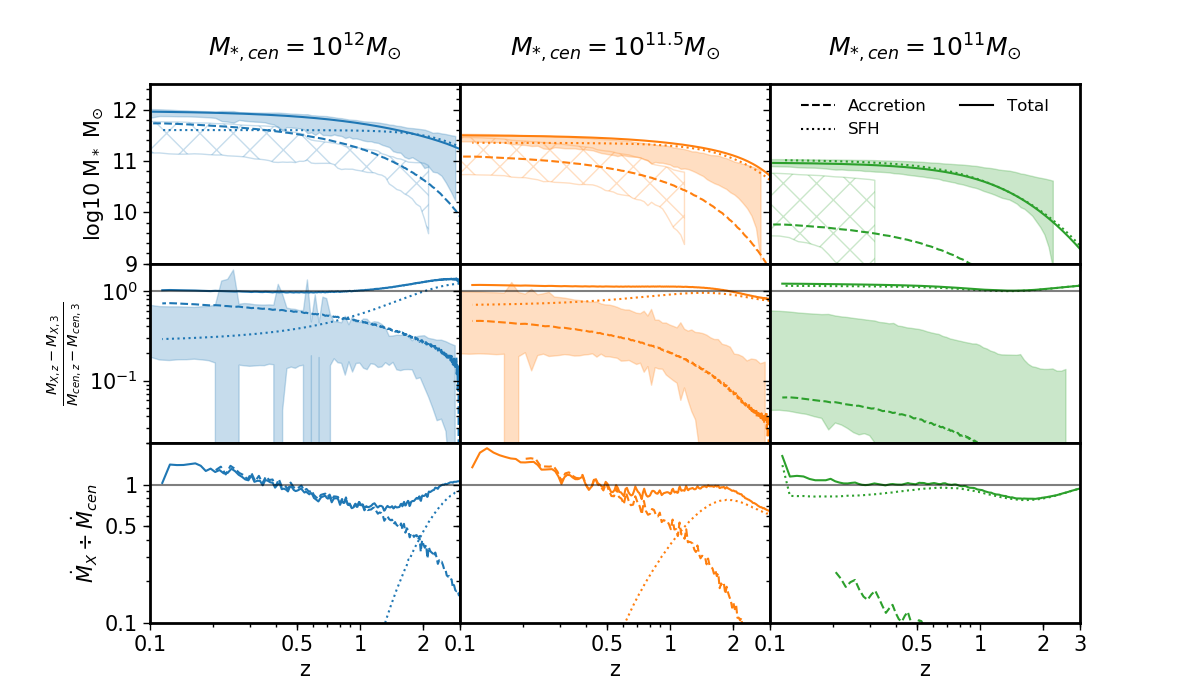
\includegraphics[width = \linewidth]{Appendices/StellarMassAssembly/SatelliteAccretion_G19_ill.png}
    \caption{As in Figure \ref{fig:SatelliteAccretion} three `mass tracks' are shown that have central galaxy masses at redshift $z = 0.1$ of $M_{*,cen}$ = $10^{12}$, $10^{11.5}$, and $10^{11}$ $[M_{\odot}]$ in blue orange and green respectively. The satellite galaxy accretion is shown for evolved satellites with a dashed line and the mass from star formation shown with a dotted line. The top panel shows the total mass of the central (solid line) and the total mass gained from accretion or star formation. The middle panel shows the fraction of the total galaxy mass formed from satellite accretion or star formation since redshift $z=3$. The bottom panel shows the ratio of the mass accretion rate from satellite galaxies the star formation rate and the mass growth rate of the central galaxy predicted by abundance matching. In the top panel the shaded regions are galaxies selected from the Illustris simulation the hashed region is then the satellite accretion from Illustris, in the middle panel the shaded region is the ratio of satellite accretion from Illustris. The grey lines in the second and third panel are at unity, the solid lines showing the sum of the other two factors should therefore be close to or on these lines.}
	\label{fig:SatelliteAccretion_ill}
\end{figure*}

In Figure \ref{fig:SatelliteAccretion_EMERGE} we show the in-situ vs ex-situ growth with the same model as shown in Figure \ref{fig:SatelliteAccretion}, we add to this plot data from the \textsc{emerge} model from \citet{Moster2018Emerge10} shown as black lines. The solid lines show the total galaxy mass followed back selecting populations by mass at redshift $z = 0.1$. The dotted and dashed lines show the amount of galaxy mass formed in-situ and ex-situ respectively. In all cases \textsc{emerge} predicts satellite accretion becomes the dominant mass growth pathway at higher redshifts then \textsc{steel}. In the third column we see that \textsc{emerge} and \textsc{steel} also disagree about the mass growth history of $log 10 M_{*,cen}$ = 11 galaxies, however, both models agree that the dominant mass growth path of galaxies at this mass are in-situ processes.

\begin{figure}
	\centering
	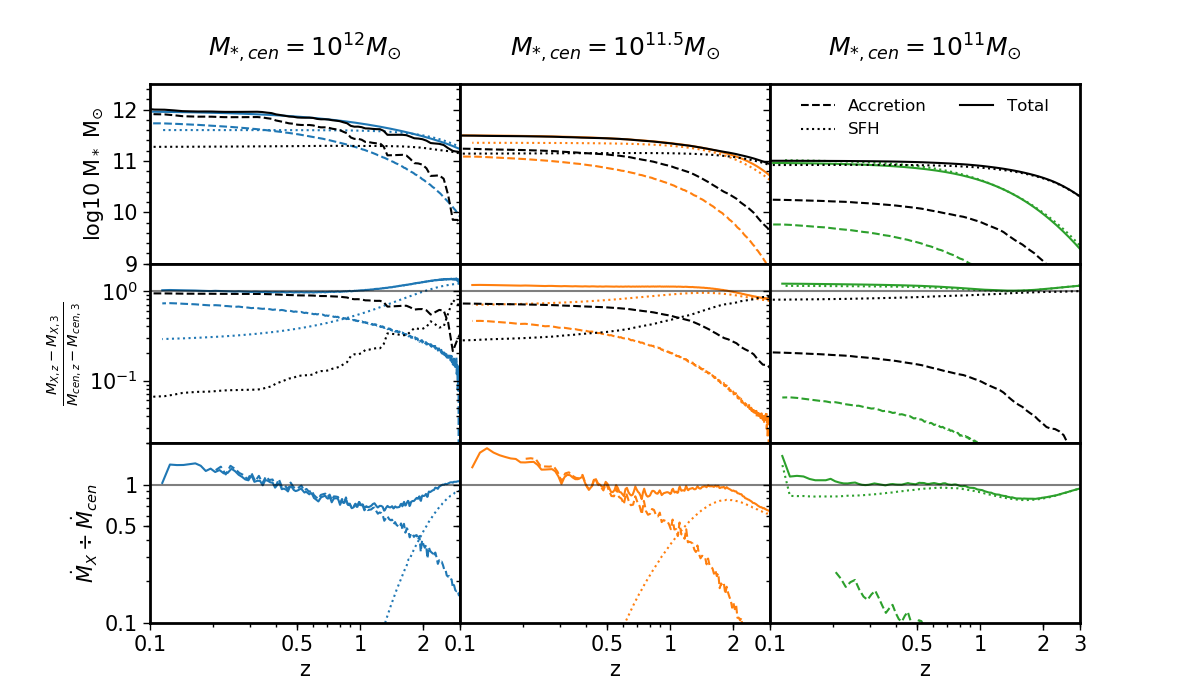
\includegraphics[width = \linewidth]{Appendices/StellarMassAssembly/SatelliteAccretion_EMERGE.png}
    \caption{As in Figure \ref{fig:SatelliteAccretion} three `mass tracks' are shown that have central galaxy masses at redshift $z = 0.1$ of $M_{*,cen}$ = $10^{12}$, $10^{11.5}$, and $10^{11}$ $[M_{\odot}]$ in blue orange and green respectively. The satellite galaxy accretion is shown for evolved satellites with a dashed line and the mass from star formation shown with a dotted line. The top panel shows the total mass of the central (solid line) and the total mass gained from accretion or star formation. The middle panel shows the fraction of the total galaxy mass formed from satellite accretion or star formation since redshift $z=3$. The bottom panel shows the ratio of the mass accretion rate from satellite galaxies the star formation rate and the mass growth rate of the central galaxy predicted by abundance matching. In the top and middle rows we add black lines to show the in-situ and ex-situ growth from \textsc{emerge} \citet{Moster2018Emerge10}. The grey lines in the second and third panel are at unity, the solid lines showing the sum of the other two factors should therefore be close to or on these lines.}
	\label{fig:SatelliteAccretion_EMERGE}
\end{figure}

In Figure \ref{fig:SatelliteAccretion_UniM} we show for the $log 10 M_{*,cen}$ = 11.5, and 11 galaxies the central growth and star formation rate ratio from \citet{Behroozi2019UniverseMachine:010}. The central growth is close to that found from \textsc{steel} and the star formation rate transition for  $log 10 M_{*,cen}$ = 11.5 is an excellent match.

\begin{figure*}
	\centering
	\includegraphics[width = \linewidth]{Appendices/StellarMassAssembly/SatelliteAccretion_UniM.png}
    \caption{As in Figure \ref{fig:SatelliteAccretion} three `mass tracks' are shown that have central galaxy masses at redshift $z = 0.1$ of $M_{*,cen}$ = $10^{12}$, $10^{11.5}$, and $10^{11}$ $[M_{\odot}]$ in blue orange and green respectively. The satellite galaxy accretion is shown for evolved satellites with a dashed line and the mass from star formation shown with a dotted line. The top panel shows the total mass of the central (solid line) and the total mass gained from accretion or star formation. The middle panel shows the fraction of the total galaxy mass formed from satellite accretion or star formation since redshift $z=3$. The bottom panel shows the ratio of the mass accretion rate from satellite galaxies the star formation rate and the mass growth rate of the central galaxy predicted by abundance matching. In the top and bottom rows, for the $log 10 M_{*,cen}$ = 11.5, and 11, we add black lines to show the central galaxy growth and the star formation rate ratio from \citet{Behroozi2019UniverseMachine:010}. The grey lines in the second and third panel are at unity, the solid lines showing the sum of the other two factors should therefore be close to or on these lines.}
	\label{fig:SatelliteAccretion_UniM}
\end{figure*}

In Figure \ref{fig:SatelliteAccretion_Menci} we show a comparison with the Semi-Analytic model described in \citet{Menci2014TriggeringInteractions}. At all masses the stellar growth is substantially different to \textsc{steel} and the other models shown in this appendix. Furthermore the Semi-Analytic model shows little change in the accreted mass ratio over cosmic time, again this is inconsistent with the findings from \textsc{steel} and the other models presented in this section. We attribute most of the differences seen here to the substantial difference in the SMHM relationship between the two models.

\begin{figure*}
	\centering
	\includegraphics[width = \linewidth]{Appendices/StellarMassAssembly/SatelliteAccretion_Menci.png}
    \caption{As in Figure \ref{fig:SatelliteAccretion} three `mass tracks' are shown that have central galaxy masses at redshift $z = 0.1$ of $M_{*,cen}$ = $10^{12}$, $10^{11.5}$, and $10^{11}$ $[M_{\odot}]$ in blue orange and green respectively. The satellite galaxy accretion is shown for evolved satellites with a dashed line and the mass from star formation shown with a dotted line. The top panel shows the total mass of the central (solid line) and the total mass gained from accretion or star formation. The middle panel shows the fraction of the total galaxy mass formed from satellite accretion or star formation since redshift $z=3$. The bottom panel shows the ratio of the mass accretion rate from satellite galaxies the star formation rate and the mass growth rate of the central galaxy predicted by abundance matching. In the top and middle rows we add black lines to show the ex-situ growth and central growth from the Semi-Analytic model described in \citet{Menci2014TriggeringInteractions}. The grey lines in the second and third panel are at unity, the solid lines showing the sum of the other two factors should therefore be close to or on these lines.}
	\label{fig:SatelliteAccretion_Menci}
\end{figure*} % Stellar Mass Assembly

\chapter{Parameter cross-sections from abundance matching MCMC.}

\label{Appx:AbnMCMC}
\lhead{\emph{Abundance Matching parameter cross-sections}}

Figure \ref{fig:MCMC_lz} shows the redshift $z = 0.1$ output from the MCMC abundance matching fits. It becomes immediately obvious that the low mass slope ($\beta$) is poorly constrained however the impact on the SMF is limited within the margin of error. The position of the knee (M) is well constrained against both the normalisation (N) and the high mass slope ($\gamma$). The shape of the constraint between the normalisation and gamma emanates from the need to produce high mass galaxies, if the normalisation is decreased the slope must increase to ensure enough haloes produce massive galaxies.

\begin{figure*}
	\centering
	\includegraphics[width = \linewidth]{Appendices/AbnMCMC/MCMC_plot_lz.png}
    \caption{We show the MCMC parameter space for the redshift $z = 0.1$ fit. The position of the knee (M), the normalisation (N) the low mass slope ($\beta$) and the high mass slope ($\gamma$) are shown from left to right. Columns are titled with the best fit values and 16th/84th percentile errors. The black lines show the best fit value with a black square at intersections, the 16th/84th percentiles are shown with blue dashed lines on the histograms.}
	\label{fig:MCMC_lz}
\end{figure*}

Figure \ref{fig:MCMC_hz} shows the redshift $z > 0.1$ output from the MCMC abundance matching fits. All parameters have low evolution and the SMHM relation evolves only weakly with redshift. For M, $\beta$, and $\gamma$ where the distributions are wide  or close to the prior we have tested wider priors and insignificant change is found.

\begin{figure*}
	\centering
	\includegraphics[width = \linewidth]{Appendices/AbnMCMC/MCMC_plot_hz.png}
    \caption{We show the MCMC parameter space for the high redshift $z > 0.1$ fit. The evolution of: the position of the knee ($M_z$), the normalisation ($N_z$) the low mass slope ($\beta_z$) and the high mass slope ($\gamma_z$) are shown from left to right. Columns are titled with the best fit values and 16th/84th percentile errors. The black lines show the best fit value with a black square at intersections, the 16th/84th percentiles are shown with blue dashed lines on the histograms.}
	\label{fig:MCMC_hz}
\end{figure*} % AbnMCMC

% Appendix FullTexts

\chapter{Full publication text}
\label{Appx:Papers}
\lhead{Full papers}

The PDFs of the three published papers are provided in full in order of publication. Papers one \cite{Grylls2019AClusters} and two \cite{Grylls2020PredictingSTEEL} are the prints from MNRAS Paper 3 \cite{Grylls2020TheFractions} is the preprint from arXiv.

\includepdf[pages=-]{Appendices/Full_PDFs/Papers/MNRAS_Final_P1.pdf}
\includepdf[pages=-]{Appendices/Full_PDFs/Papers/MNRAS_Final_P2.pdf}
\includepdf[pages=-]{Appendices/Full_PDFs/Papers/arXiv_P3.pdf}
	% Full Papers

% Appendix HF

\chapter{Fellowship Application and future of \steel}
\label{Appx:HF}
\lhead{Future}

This is PJG's unsuccessful but well reviewed (4/6, 4/6, 6/6) fellowship application. Included are original submission documents, all reviewers reports and PJG's response. These documents represent PJG's technical vision for this project.

\includepdf[pages=-]{Appendices/Full_PDFs/HF/Hawking_Fellowship_Case_for_support.pdf}
\includepdf[pages=-]{Appendices/Full_PDFs/HF/Hawking_Fellowship_Pathways_to_Impact.pdf}
\includepdf[pages=-]{Appendices/Full_PDFs/HF/Hawking_Fellowship_PERT.pdf}	% HF

%\input{./Appendices/AppendixB} % Appendix Title

%\input{./Appendices/AppendixC} % Appendix Title

\addtocontents{toc}{\vspace{2em}}  % Add a gap in the Contents, for aesthetics
\backmatter

%% ----------------------------------------------------------------
\label{Bibliography}
\lhead{\emph{Bibliography}}  % Change the left side page header to "Bibliography"
\bibliographystyle{unsrtnat}  % Use the "unsrtnat" BibTeX style for formatting the Bibliography
\bibliography{Mendeley}  % The references (bibliography) information are stored in the file named "Bibliography.bib"

\end{document}  % The End
%% ----------------------------------------------------------------